% !TEX program = pdflatex
% CableTract --- Prototype-Free Feasibility Study
% Compile: pdflatex cabletract_manuscript.tex (twice for cross-refs)

\documentclass[11pt,a4paper]{article}

% --------------------------------------------------------------------
% Packages
% --------------------------------------------------------------------
\usepackage[utf8]{inputenc}
\usepackage[T1]{fontenc}
\usepackage{lmodern}
\usepackage[english]{babel}
\usepackage[a4paper,margin=2.4cm]{geometry}
\usepackage{microtype}
\usepackage{amsmath,amssymb,amsthm}
\usepackage{mathtools}
\usepackage{siunitx}
\usepackage{graphicx}
\usepackage{float}
\usepackage{booktabs}
\usepackage{longtable}
\usepackage{array}
\usepackage{multirow}
\usepackage{tabularx}
\usepackage{caption}
\usepackage{subcaption}
\usepackage{xcolor}
\usepackage{enumitem}
\usepackage{tikz}
\usetikzlibrary{positioning,calc,arrows.meta,decorations.pathreplacing,backgrounds,shapes.geometric,fit,patterns}
\usepackage[hidelinks,colorlinks=true,linkcolor=blue!60!black,citecolor=blue!60!black,urlcolor=blue!60!black]{hyperref}
% Render \textsubscript (e.g. CO_2) and \textsuperscript as plain text in PDF
% bookmarks/headings, so hyperref does not warn on tokens it cannot expand.
\pdfstringdefDisableCommands{\def\textsubscript#1{#1}\def\textsuperscript#1{#1}}
\usepackage[nameinlink,capitalise]{cleveref}
\usepackage[acronym,nonumberlist,nopostdot,toc]{glossaries}

\graphicspath{{figures/}}

% siunitx setup
\sisetup{
    detect-all,
    per-mode = symbol,
    range-phrase = --,
    range-units = single,
    group-separator = {\,},
    group-minimum-digits = 4
}
\DeclareSIUnit{\decare}{decare}
\DeclareSIUnit{\hectare}{ha}
\DeclareSIUnit{\litre}{L}
\DeclareSIUnit{\year}{yr}
\DeclareSIUnit{\Wh}{Wh}
\DeclareSIUnit{\kWh}{kWh}
\DeclareSIUnit{\auger}{augers}
\DeclareSIUnit{\EUR}{EUR}
\DeclareSIUnit{\USD}{USD}
\DeclareSIUnit{\hp}{hp}

% Repository for the analytical implementation
\newcommand{\cabletractrepo}{\url{https://github.com/yilmazozgur/cabletract}}

% Caption style
\captionsetup{font=small,labelfont=bf,format=plain,justification=raggedright,singlelinecheck=false}

% Tighter table notes
\newcommand{\tabnote}[1]{{\footnotesize\textit{Note.} #1}}

% Section spacing
\usepackage{titlesec}
\titleformat{\section}{\normalfont\Large\bfseries}{\thesection}{0.6em}{}
\titleformat{\subsection}{\normalfont\large\bfseries}{\thesubsection}{0.6em}{}
\titleformat{\subsubsection}{\normalfont\normalsize\bfseries}{\thesubsubsection}{0.6em}{}
\titlespacing*{\section}{0pt}{1.4ex}{0.7ex}
\titlespacing*{\subsection}{0pt}{1.1ex}{0.5ex}
\titlespacing*{\subsubsection}{0pt}{0.9ex}{0.4ex}

% --------------------------------------------------------------------
% Acronym glossary --- every acronym used in the paper, defined here
% so the first use in the body expands automatically via \gls{}.
% --------------------------------------------------------------------
\makeglossaries

% Domain & standards
\newacronym{asabe}{ASABE}{American Society of Agricultural and Biological Engineers}
\newacronym{iwrc}{IWRC}{Independent Wire Rope Core}
\newacronym{ice}{ICE}{Internal Combustion Engine}
\newacronym{icedb}{ICE-DB\,v3}{Inventory of Carbon and Energy database, version 3 (Hammond \& Jones)}
\newacronym{ctf}{CTF}{Controlled Traffic Farming}
\newacronym{cdpr}{CDPR}{Cable-Driven Parallel Robot}
\newacronym{wd}{4WD}{Four-Wheel Drive}
\newacronym{lca}{LCA}{Life-Cycle Assessment}
\newacronym{lco}{LCO}{Levelised Cost of Operation (EUR per hectare-year)}
\newacronym{npv}{NPV}{Net Present Value}
\newacronym{capex}{CAPEX}{Capital Expenditure}
\newacronym{bom}{BoM}{Bill of Materials}
\newacronym{bos}{BoS}{Balance of System (PV cabling, mounting, inverter)}
\newacronym{eu}{EU}{European Union}
\newacronym{dem}{DEM}{Discrete Element Method}
\newacronym{mpc}{MPC}{Model-Predictive Control}
\newacronym{pid}{PID}{Proportional--Integral--Derivative (control)}

% Powertrain & hardware
\newacronym{pmsm}{PMSM}{Permanent-Magnet Synchronous Motor}
\newacronym{bldc}{BLDC}{Brushless DC motor}
\newacronym{pv}{PV}{Photovoltaic}
\newacronym{vawt}{VAWT}{Vertical-Axis Wind Turbine}
\newacronym{soc}{SoC}{State of Charge}
\newacronym{bms}{BMS}{Battery Management System}
\newacronym{gnss}{GNSS}{Global Navigation Satellite System}
\newacronym{gps}{GPS}{Global Positioning System}

% Energy / weather data sources
\newacronym{tmy}{TMY}{Typical Meteorological Year}
\newacronym{ghi}{GHI}{Global Horizontal Irradiance}
\newacronym{doy}{DOY}{Day Of Year}
\newacronym{nrel}{NREL}{(US) National Renewable Energy Laboratory}
\newacronym{nsrdb}{NSRDB}{(NREL) National Solar Radiation Database}
\newacronym{pvgis}{PVGIS}{(EU JRC) Photovoltaic Geographical Information System}
\newacronym{sarah}{SARAH2}{Surface Solar Radiation Data Set --- Heliosat, version 2}
\newacronym{niwe}{NIWE}{(India) National Institute of Wind Energy}
\newacronym{inmet}{INMET}{(Brazil) National Institute of Meteorology}
\newacronym{swera}{SWERA}{Solar and Wind Energy Resource Assessment}

% Statistical & ML
\newacronym{p10}{P10}{10th percentile of a sampled distribution}
\newacronym{p50}{P50}{50th (median) percentile of a sampled distribution}
\newacronym{p90}{P90}{90th percentile of a sampled distribution}
\newacronym{gbt}{GBT}{Gradient-Boosted Trees (regression)}
\newacronym{gbr}{GBR}{Gradient Boosting Regressor (scikit-learn)}
\newacronym{nsga}{NSGA-II}{Non-dominated Sorting Genetic Algorithm, version II}
\newacronym{salib}{SALib}{Sensitivity Analysis Library (Python)}
\newacronym{sobol1}{S1}{Sobol first-order sensitivity index}
\newacronym{sobolt}{ST}{Sobol total-order sensitivity index}
\newacronym{rmse}{RMSE}{Root Mean Squared Error}
\newacronym{r2}{R\textsuperscript{2}}{Coefficient of determination}

% Data, agencies, methods
\newacronym{fem}{FEM}{Finite Element Method}
\newacronym{usda}{USDA NASS}{(US) Department of Agriculture, National Agricultural Statistics Service}
\newacronym{defra}{DEFRA}{(UK) Department for Environment, Food \& Rural Affairs}
\newacronym{eea}{EEA}{European Environment Agency}
\newacronym{ivl}{IVL}{IVL Swedish Environmental Research Institute}
\newacronym{inrae}{INRAE}{French National Research Institute for Agriculture, Food and Environment}
\newacronym{dlg}{DLG}{Deutsche Landwirtschafts-Gesellschaft}
\newacronym{bnef}{BloombergNEF}{Bloomberg New Energy Finance}
\newacronym{api}{API}{Application Programming Interface}

% Concepts unique to this paper
\newacronym{mu}{MU}{Main Unit (winch + motor + battery + energy-harvester module)}
\newacronym{rq}{RQ}{Research Question}
\newacronym{c1}{C1}{compaction-reduction claim}
\newacronym{c2}{C2}{energy-reduction claim}
\newacronym{c3}{C3}{off-grid-feasibility claim}
\newacronym{c4}{C4}{economics and life-cycle CO\textsubscript{2} claim}

% --------------------------------------------------------------------
% Title block
% --------------------------------------------------------------------
\title{\textbf{CableTract: A Co-Designed Cable-Driven Field Robot for\\
Low-Compaction, Off-Grid Capable Agriculture}\\[0.4em]
\large A Prototype-Free Feasibility Framework and Analytical Envelope%
\thanks{A preliminary version of this work is available as a preprint: \texttt{arXiv:2604.09938}.}}
\author{Özgür Yılmaz\\[0.3em]
\normalsize Adana Alparslan Türkeş Science and Technology University, Adana, Türkiye\\[0.15em]
\normalsize \texttt{ozguryilmaz@atu.edu.tr}}
\date{July 2026}

% Glossary section heading customisation
\renewcommand{\acronymname}{List of acronyms}

\begin{document}
\maketitle

\begin{abstract}
\noindent
Tractor mass, not implement mass, sets the soil-compaction cost of conventional field operations, and on light and medium operations it also carries a large share of the energy cost. We present \textbf{CableTract}, a prototype-free feasibility study of a two-module cable-driven field robot: a stationary Main Unit and a lighter ground-screw-anchored Anchor module tension a cable across a strip while a soil-supported, cable-towed ${\approx}\SI{250}{\kilogram}$ implement carriage does the work, keeping the heavy bodies on fixed traffic lanes at the strip ends. The central design lever is a 10-implement library \emph{co-designed} for the architecture --- narrower, slower, shallower and lighter than tractor implements. An open, reproducible pipeline couples catenary, anchoring and drivetrain mechanics (including the energy of re-setting thirteen ground screws every strip), \gls{asabe} D497.7 draft estimates, an hourly solar/wind/battery simulator with multi-day cloud persistence on six climate sites, a coverage planner, a contact-pressure compaction model, discounted-cash-flow economics with life-cycle CO\textsubscript{2}, and global sensitivity analysis; five higher-fidelity studies --- a nonlinear $p$--$y$ anchoring model, a closed-loop depth-control co-simulation, a cable-safety model, a soil--tool discrete-element model, and a co-design robustness sweep --- stress-test the load-bearing assumptions. Under the reference assumptions the architecture roughly \emph{halves} trafficked area at $4.6\times$ lower contact pressure (a ${\sim}39\times$ field-integrated reduction in the $p^2$-weighted soil-stress exposure), uses ${\sim}2.9\times$ less useful energy than an \SI{80}{hp} diesel tractor (${\sim}10\times$ less primary fuel energy), and is off-grid capable at high-irradiance sites (58 grid-hours per year at the sunniest bundled site, 150--282 at the other five, under a seasonal duty cycle). The replacement-frame economics are scale-conditional: approximately cost-neutral at \SI{25}{\hectare\per\year} (NPV ${\approx}\SI{-1.7}{\kilo\EUR}$, within parameter uncertainty of zero), positive above ${\sim}\SI{40}{\hectare\per\year}$, and \SI{+9.1}{\kilo\EUR} at \SI{100}{\hectare\per\year}; life-cycle CO\textsubscript{2} is $1.9\times$ lower than diesel independent of grid decarbonisation. The dominant unresolved risks are \emph{mechanical} --- anchor loading, depth control, lateral guidance and cable safety --- which the studies bound but a prototype must ultimately test: a consistent analytical envelope for a future prototype, not a validated machine.

\medskip
\noindent\textbf{Keywords:} cable-driven robot; soil compaction; controlled traffic farming; implement co-design; off-grid agriculture; techno-economic analysis; feasibility modelling.
\end{abstract}

\tableofcontents

% Reset acronym first-use flags so the body (not the abstract) gets the
% first expanded form of each \gls{} acronym.
\glsresetall

% ====================================================================
\section{Introduction}\label{sec:intro}
% ====================================================================

A modern \SI{80}{hp} \gls{wd} utility tractor weighs ${\approx}\SI{4}{\tonne}$, while the implements it tows are typically \SIrange{0.2}{1.5}{\tonne}. Each pass therefore drags several times more body mass than tool mass across the field, paying a soil-compaction penalty --- mean contact pressures of \SIrange{100}{250}{\kilo\pascal}~\cite{keller2010compaction}, well above the ${\sim}\SI{50}{\kilo\pascal}$ subsoil-stress limit commonly recommended for wet fine-textured soils~\cite{schjonning2012rules} --- and burning ${\approx}\SI{12}{\litre\per\hectare}$ of diesel on a mid-range field operation~\cite{siemens1999machinery,asabe-d497}. For a single such operation per year on a \SI{25}{\hectare} farm this is \SI{4500}{\litre} of diesel and ${\approx}\SI{12}{\tonne}$ of combustion CO\textsubscript{2} over a 15-year machine life; a full multi-operation calendar is several times that.

CableTract attacks the dead-weight problem at the \emph{architectural} level rather than the powertrain level. Two modules sit at opposite ends of a strip: a \textbf{Main Unit} carrying the winch, motor, controller, battery, \gls{pv} array, and small wind turbine; and an \textbf{Anchor} resisting the cable reaction with retractable ground screws. A lightweight implement carriage --- soil-supported on wide rollers and \emph{towed} by the cable --- runs between them. Only the carriage traffics the field interior; the heavy modules move along fixed lanes at the strip ends (one lane per \SI{50}{\meter} coverage band on deeper fields), stepping by one strip width per round. Replacing the heavy traction body with a tensioned cable changes three things at once: (i) the field interior is trafficked only by the carriage's low-pressure rollers; (ii) the energy budget no longer carries a \SI{4}{\tonne} body; (iii) the Main Unit, being nearly stationary, can carry deployable \gls{pv} and a small wind turbine more easily than a fully mobile electric tractor. In compaction terms the architecture is best understood as an extreme form of \gls{ctf}~\cite{tullberg2007ctf,chamen2015mitigating}: it confines all high-pressure traffic to fixed lanes, and its incremental contribution over \gls{ctf} with an existing tractor is the off-grid electric energy system and the light in-field footprint, not the lane discipline itself.

The natural objection is that this only works if the implements are also redesigned. A conventional 8-row planter or a \SI{3}{\meter} disk harrow is built to be towed by a \SI{4}{\tonne} tractor; it expects high draft and high speed. Towing those \emph{unmodified} implements with a cable robot is the wrong problem. The right problem is to \textbf{co-design the carriage and a small library of implements together}: narrow strip widths matched to the cable swath, slower operating speeds that avoid the speed-dependent terms of the soil-draft equation, shallower depths that match what a carriage-mounted tool can resist, and lighter implement frames freed from the hitch loads of a real tractor. This co-design is the main analytical lever of the paper and we return to it explicitly in \cref{sec:codesign,sec:soil}.

The contribution is not an experimental validation. It is a \textbf{prototype-free, fully reproducible feasibility envelope} that asks one question:

\begin{quote}
\itshape Under what (climate $\times$ farm size $\times$ operation type) conditions does a co-designed cable-driven field robot beat a conventional diesel tractor on energy, compaction, \gls{npv}, and life-cycle CO\textsubscript{2} --- when can it do so off-grid --- and where doesn't it?
\end{quote}

We answer it with an open analytical pipeline\footnote{\cabletractrepo} that runs end-to-end from a clean checkout, ships with all input data bundled (no live \gls{api} calls), and regenerates every figure and table in this paper from the phase scripts (\texttt{run\_phase1}--\texttt{run\_phase12}, plus \texttt{run\_phase6b}). \Cref{sec:related} positions the architecture against cable traction, \gls{ctf} and gantry systems, and adjacent field robots; \cref{sec:concept} defines the system concept and the co-designed implement library; \cref{sec:methods} walks through the model in the order in which the figures are generated; \cref{sec:results} reports the results against four explicit claims; and \cref{sec:discussion} closes the envelope with the binding constraints.

\paragraph{Key results (codesigned reference).} Each is conditional on the workload and purchase frame stated in the body:
\begin{itemize}[leftmargin=1.4em,itemsep=0.12em]
    \item \textbf{Energy:} \SI{1227}{\Wh\per\decare}\footnote{One decare $=0.1$\,ha $=1000\,\si{\meter\squared}$; \SI{1}{\Wh\per\decare} $=\SI{10}{\Wh\per\hectare}$.} (\SI{12.3}{\kWh\per\hectare}) delivered electrical, of which ${\sim}27\%$ is the newly bookkept energy of re-setting the thirteen ground screws every strip (flat-field bound \SI{1259}{\Wh\per\decare} without regen) --- about $2.9\times$ less than the diesel comparator's estimated \emph{drawbar} work and ${\sim}10\times$ less than its \emph{primary fuel} energy (${\approx}\SI{120}{\kWh\per\hectare}$ at $12\,\si{\litre\per\hectare}$); most of the primary-energy factor is generic \gls{ice}-to-electric conversion, not the architecture.
    \item \textbf{Compaction:} roughly \emph{half} the trafficked area (${\approx}27\%$ vs ${\approx}50\%$ of field area per pass) at a $4.6\times$ lower mean contact pressure (31 vs \SI{143}{\kilo\pascal}), giving a ${\sim}39\times$ lower field-integrated $p^2$-weighted exposure and a ${\sim}73\times$ lower per-running-gear contact-energy index.
    \item \textbf{Off-grid:} under a seasonal 170-day duty cycle the reference hardware (\SI{15}{\meter\squared} \gls{pv} + \SI{9}{\kWh}) needs 58 grid-hours per year at the sunniest bundled site (Konya) and \SIrange{150}{282}{\hour\per\year} at the other five --- \emph{climate-conditional but nowhere categorical}; per-site daily coverage on harvested energy alone has medians of \SIrange{6.5}{9.3}{decares\per day}.
    \item \textbf{Economics (replacement frame, machine capex \SI{38670}{\EUR} vs \SI{35000}{\EUR}):} scale-conditional. \gls{npv} vs diesel at 8\,\% is ${\approx}\SI{-1.7}{\kilo\EUR}$ at \SI{25}{\hectare\per\year} (cost-neutral within parameter uncertainty), turns positive near \SI{40}{\hectare\per\year}, and reaches \SI{+9.1}{\kilo\EUR} at \SI{100}{\hectare\per\year}. In the \emph{additive} frame (full system incl.\ implements financed, no tractor retired) the \SI{25}{\hectare} \gls{npv} is ${\approx}\SI{-61}{\kilo\EUR}$ and a single machine cannot amortise itself within its own ${\approx}\SI{200}{\hectare\per\year}$ capacity.
    \item \textbf{Life-cycle CO\textsubscript{2}:} \SI{17.0}{\kilogram\per\hectare\per\year} versus 32.5 (diesel) and 27.9 (electric tractor) --- a $1.9\times$ improvement over diesel independent of grid decarbonisation.
\end{itemize}

% ====================================================================
\section{Related Work}\label{sec:related}
% ====================================================================

\subsection{Prior cable traction: steam cable ploughing, forestry winches, and the Orlando--Zoffoli patent}\label{sec:related-cable}

Cable-driven field machines are not new --- they are, in fact, one of the oldest forms of mechanised tillage. \textbf{Steam cable ploughing} was deployed at scale in the second half of the 19th century, particularly on heavy clays in the United Kingdom and continental Europe: two stationary steam engines at opposite headlands pulled a balance plough back and forth on a steel cable (the Fowler and Howard systems)~\cite{tyler1970steam,lane1980fowler}. The system coexisted with horse and traction-engine ploughing for decades and then disappeared by the early 20th century; the historical record attributes the decline to per-station crew overhead, the time cost of repositioning the engines after each strip, the management burden of the cable itself, and the inability to turn at the headland and resume continuously~\cite{tyler1970steam}. CableTract automates the crew problem (both modules are autonomous) and this paper quantifies the repositioning cost explicitly (\cref{sec:anchoring-energy,sec:layout-findings}); cable management and continuous operation remain open risks that we carry in \cref{sec:open-risks}. A second, commercially mature modern analogue is \textbf{winch-assist (tethered) forestry harvesting}, which anchors a winch machine and tensions a cable to a working machine on steep slopes --- a directly transferable body of practice on anchoring, synthetic-rope handling, and repeated winch cycles.

The closest published agricultural prior art is \textbf{US 8,763,714 B2}~\cite{orlando2014patent} (Orlando \& Zoffoli), which describes a cable traction system using two technically \emph{identical} electric machines, each with a hoist and stabilisation, with the implement moving between them as cable is wound and unwound. The patent motivates the design through reduced soil degradation and electric propulsion, and includes a telescopic arm for cable placement during repositioning. On the robotics side, the CableTract+ variant of \cref{sec:variant-plus} belongs to the well-studied \gls{cdpr} family --- planar cable robots with multiple winch stations~\cite{pott2018cdpr}, from the NIST RoboCrane~\cite{albus1993robocrane} to cable-suspended agricultural sensing platforms such as the ETH field phenotyping platform~\cite{kirchgessner2017fip}; CableTract's single-cable strip architecture is a deliberately reduced member of that family, trading workspace dimensionality for anchor simplicity.

CableTract overlaps with the Orlando--Zoffoli family but differs in three structural ways:

\begin{enumerate}[leftmargin=1.6em,itemsep=0.2em]
    \item \textbf{Asymmetric architecture.} CableTract uses a heavy \gls{mu} (\gls{pmsm}, controller, battery, PV/wind energy harvester) and a much lighter Anchor (ground-screw drives, sensors). The Anchor needs no winch and no high-power electronics, which roughly halves its \gls{bom}.
    \item \textbf{Ground-screw anchoring.} Cable reaction is resisted by retractable ground screws driven into the soil rather than by the machine's mass alone. This is what makes the lighter Anchor module geotechnically defensible (\cref{sec:anchor}); helical anchor design practice is well documented~\cite{perko2009helical,ac358}.
    \item \textbf{Co-designed implements.} CableTract is paired with an implement library sized for the cable architecture, not borrowed from tractor inventories (\cref{sec:codesign}).
\end{enumerate}

We do \emph{not} claim CableTract is the first cable-driven agricultural machine. The contribution is an analytical evaluation of the asymmetric \gls{mu}\,+\,Anchor architecture under co-designed implements, and the identification of the operating envelope in which it is genuinely competitive.

\subsection{Controlled traffic farming and gantry systems: the incumbent compaction solutions}\label{sec:related-ctf}

Because CableTract's compaction claim is central, it must be benchmarked against the established engineering answers to compaction, not only against random-traffic diesel operation. \textbf{\Gls{ctf}} confines all machinery traffic to permanent lanes, typically reducing the trafficked fraction of the field to \SIrange{15}{30}{\percent} with the farmer's \emph{existing} tractor at modest incremental cost~\cite{tullberg2007ctf,chamen2015mitigating}. \textbf{Wide-span (gantry) vehicles} carry the implement between wheels running on permanent lanes and are the closest architectural relative of a cable robot --- heavy bodies on lanes, full-width tool between them, with no cable and no anchor-reset cycle. McPhee et al.~\cite{mcphee2020lowmass} pose exactly the question this paper inherits: whether soil compaction is better managed by low-mass autonomous vehicles or by controlled traffic. CableTract's corrected compaction numbers (\cref{sec:compaction}: ${\approx}27\%$ trafficked area per pass at \SI{31}{\kilo\pascal}) are therefore comparable to good \gls{ctf} on trafficked \emph{area}, and its genuine increments over \gls{ctf} are (i) the much lower contact pressure of the in-field running gear, (ii) the off-grid renewable energy system that a nearly stationary Main Unit can carry, and (iii) autonomy. We state this positioning explicitly to avoid claiming novelty for lane discipline itself.

\subsection{Adjacent vehicle classes}\label{sec:related-adjacent}

CableTract also sits in a design space populated by commercial field robots and electric tractors, whose economics have begun to be studied formally~\cite{lagnelov2021cost,lowenberg2020economics}. We bundle a competitor table\footnote{See \texttt{tables/competitor\_comparison.csv} in the repository; manufacturer figures are indicative, not peer-reviewed.} with public-domain reference numbers for each class (\cref{sec:competitor}). The five classes are:

\begin{itemize}[leftmargin=1.6em,itemsep=0.15em]
    \item \textbf{Conventional \SI{80}{hp} \gls{wd} diesel utility tractor} --- the cost-floor reference against which energy, compaction, and \gls{npv} are measured.
    \item \textbf{Battery-electric tractors} (Monarch MK-V, Kubota LXe-261, Solectrac eUtility) --- same form factor as a tractor but with a Li-ion pack. Solves the fuel cost but not the compaction problem; usually grid-charged.
    \item \textbf{Autonomous PV-powered field robots} (FarmDroid FD20) --- small, light, on-board solar; designed for sugar beet / row crops. Cannot do tillage. Off-grid by construction.
    \item \textbf{Autonomous solar weeders / spot sprayers} (ecoRobotix AVO class) --- narrow, light, on-board PV; weeding and spot-spraying only.
    \item \textbf{Autonomous weeders} (Naïo Oz) --- vegetable / row-crop only; no heavy draft.
\end{itemize}

Within this comparison set CableTract is the only architecture that simultaneously (a) is \emph{off-grid capable} in the sense of being self-powered from on-board renewables, (b) supports \emph{light-to-medium primary tillage} at co-designed depths, and (c) does so with a \SI{250}{\kilogram} in-field footprint rather than a \SIrange{1}{4}{\tonne} tractor body. The numerical comparison is in \cref{sec:competitor}.

% ====================================================================
\section{System Concept and Co-Design}\label{sec:concept}
% ====================================================================

\Cref{fig:f0b} shows the CableTract concept in operation: the two heavy modules rest on opposite headlands while only a tensioned cable and a lightweight implement carriage enter the field.

\begin{figure}[H]
\centering
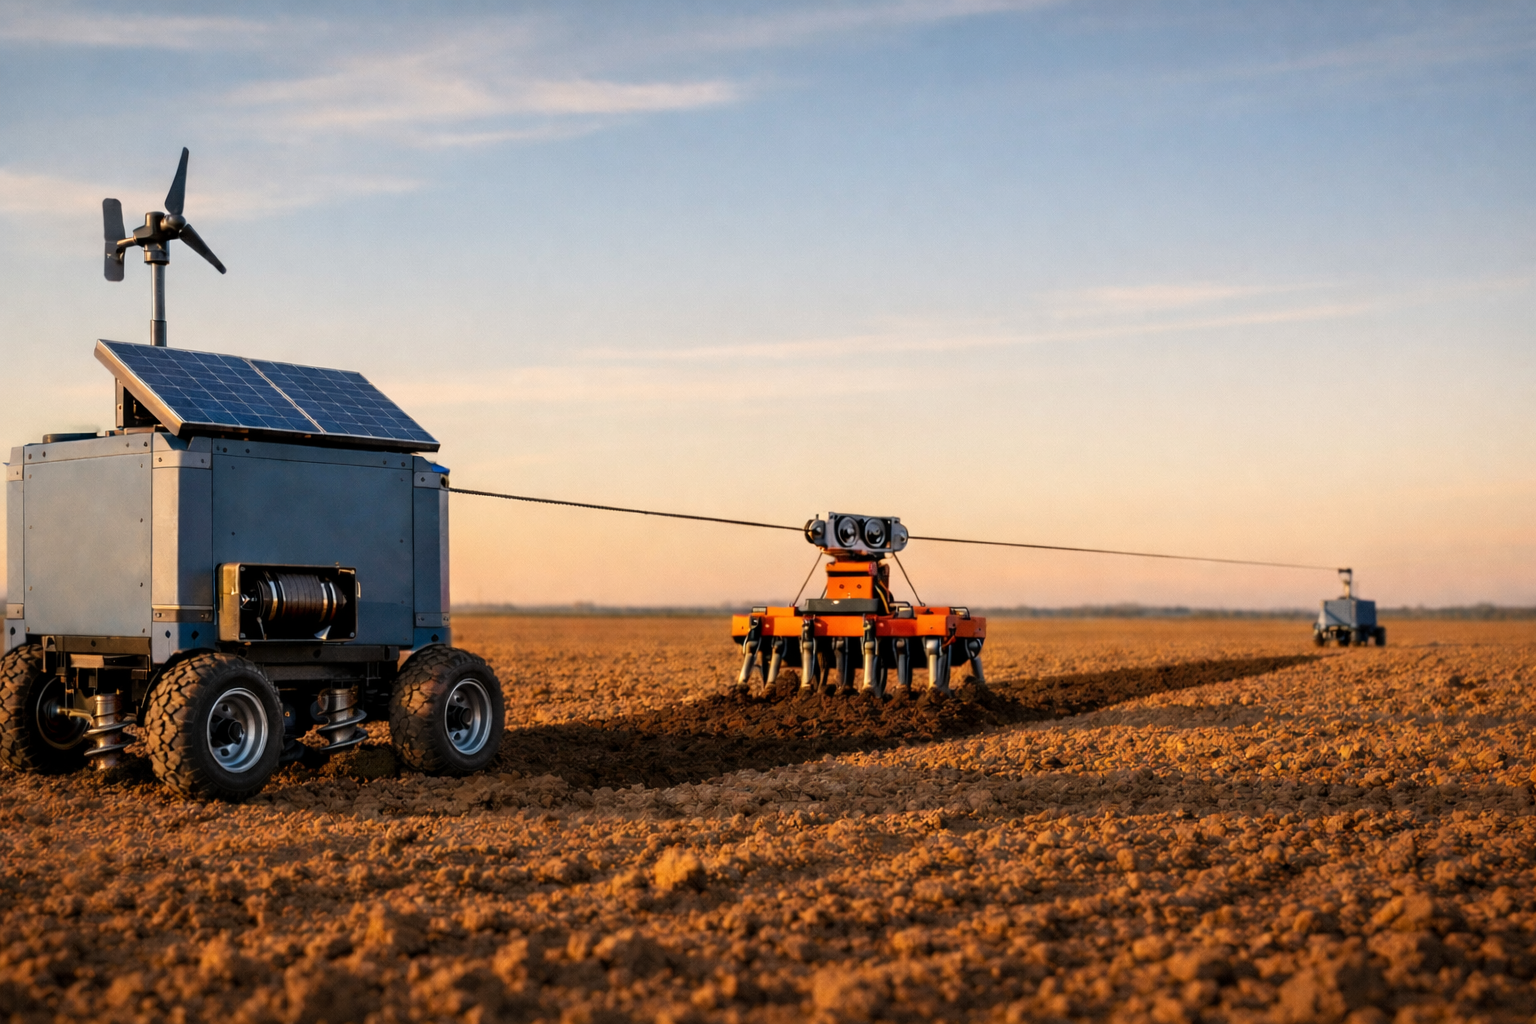
\includegraphics[width=0.92\linewidth]{F0b_hero_scene}
\caption{\textbf{Concept illustration (AI-assisted render --- no physical prototype exists; details differ from the specification, e.g.\ the render shows a horizontal-axis turbine where the design uses a \gls{vawt}, and understates cable sag).} The Main Unit (left) houses the winch, drivetrain, battery, PV panel and small wind turbine; the Anchor (right) is a passive ground-screw module that resists the cable reaction. A lightweight implement carriage --- soil-supported on wide rollers and towed by the cable --- works a typical \SI{50}{\meter} span. The field interior is trafficked only by the carriage; the two heavy modules occupy fixed lanes at the strip ends (one lane per \SI{50}{\meter} coverage band on deeper fields).}
\label{fig:f0b}
\end{figure}

\subsection{Two-module architecture}\label{sec:two-module}

\begin{figure}[H]
\centering
\resizebox{\linewidth}{!}{%
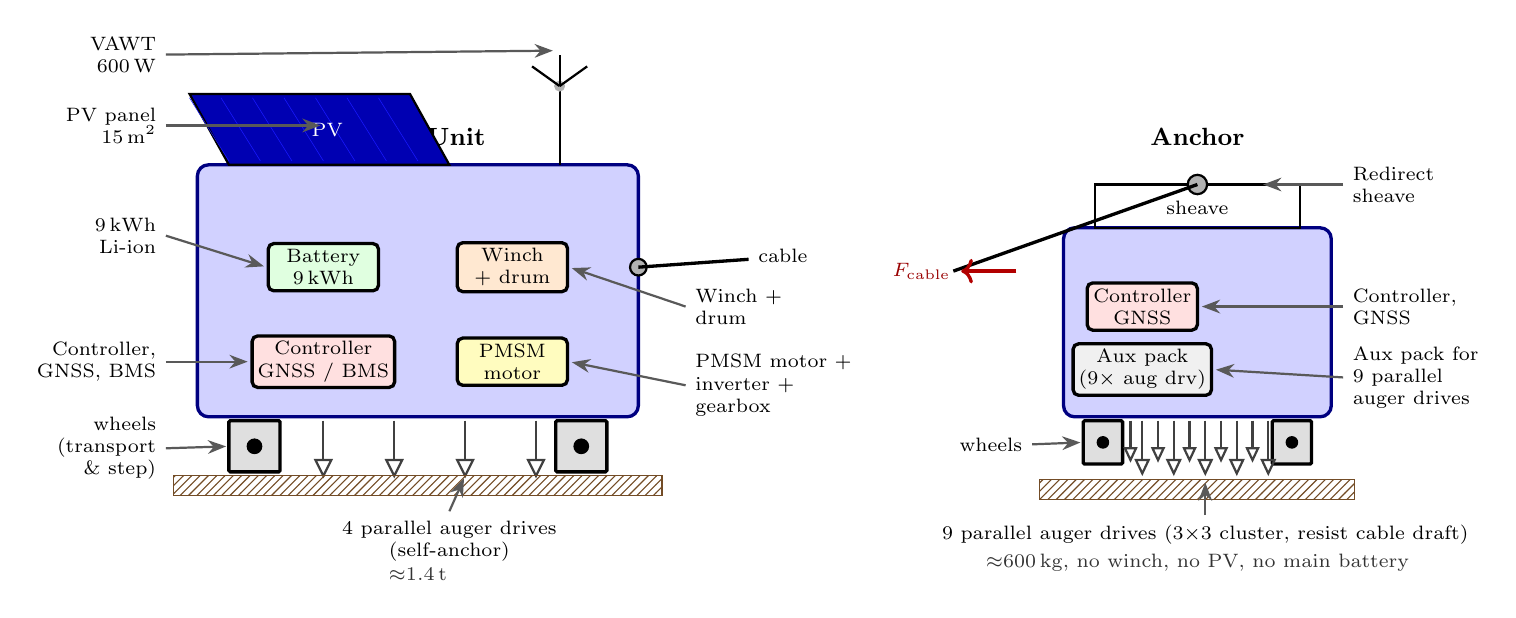
\begin{tikzpicture}[
    every node/.style={font=\footnotesize},
    subsys/.style={draw=black, very thick, rounded corners=2pt, fill=blue!8,
                   minimum width=14mm, minimum height=6mm, align=center,
                   inner sep=2pt, font=\scriptsize},
    callout/.style={->, >=Stealth, thick, gray!70!black, shorten >=1pt},
    body/.style={draw=blue!50!black, very thick, fill=blue!18, rounded corners=4pt},
    ground/.style={pattern=north east lines, pattern color=brown!60!black, draw=brown!60!black},
    wheel/.style={draw=black, very thick, fill=gray!25, rounded corners=0.5pt},
]

% =====================================================================
% LEFT PANEL: Main Unit
% =====================================================================
\begin{scope}[xshift=0cm]

% Module body (rectangle)
\draw[body] (0,0) rectangle (5.6,3.2);
\node[font=\bfseries\small] at (2.8,3.55) {Main Unit};

% PV panel on top, tilted
\draw[fill=blue!70!black, draw=black, thick]
    (0.4,3.2) -- ++(2.8,0) -- ++(-0.5,0.9) -- ++(-2.8,0) -- cycle;
\foreach \x in {0.0,0.4,0.8,1.2,1.6,2.0,2.4} {
    \draw[blue!90!white, very thin] (0.4+\x,3.25) -- (0.4+\x-0.5,4.05);
}
\node[font=\scriptsize, white] at (1.65,3.65) {PV};

% Wind turbine
\draw[thick] (4.6,3.2) -- (4.6,4.2);
\fill[gray!60] (4.6,4.2) circle (2pt);
\draw[thick] (4.6,4.2) -- ++(0.35,0.25);
\draw[thick] (4.6,4.2) -- ++(-0.35,0.25);
\draw[thick] (4.6,4.2) -- ++(0,0.4);

% Internal subsystems (boxes inside the body)
\node[subsys, fill=orange!18] (winch) at (4.0,1.9) {Winch\\+ drum};
\node[subsys, fill=yellow!25] (motor) at (4.0,0.7) {PMSM\\motor};
\node[subsys, fill=green!12] (batt)  at (1.6,1.9) {Battery\\\SI{9}{\kWh}};
\node[subsys, fill=red!12]   (ctrl)  at (1.6,0.7) {Controller\\GNSS / BMS};

% Pulley + cable exit on the right
\fill[gray!60] (5.6,1.9) circle (3pt);
\draw[thick] (5.6,1.9) circle (3pt);
\draw[very thick, black] (5.6,1.9) -- (7.0,2.0);
\node[anchor=west, font=\scriptsize] at (7.0,2.05) {cable};

% 2 wheels (transport mode + headland step) and 4 helical augers (self-anchoring)
% Wheels on the outer corners
\draw[wheel] (0.4,-0.05) rectangle (1.05,-0.7);
\fill[black] (0.725,-0.375) circle (0.1);
\draw[wheel] (4.55,-0.05) rectangle (5.2,-0.7);
\fill[black] (4.875,-0.375) circle (0.1);
% Augers between/around the wheels (deployed downward into the soil)
\foreach \x in {1.6,2.5,3.4,4.3} {
    \draw[thick, gray!50!black] (\x,-0.05) -- (\x,-0.55);
    \draw[thick, gray!50!black] (\x-0.1,-0.55) -- (\x+0.1,-0.55)
                                                -- (\x,-0.75) -- cycle;
}

% Ground line under MU
\draw[ground] (-0.3,-0.75) rectangle (5.9,-1.0);

% Callouts (external labels)
\node[anchor=east, font=\scriptsize, align=right] (lblPV) at (-0.4,3.7) {PV panel\\\SI{15}{\meter\squared}};
\draw[callout] (lblPV.east) -- (1.6,3.7);

\node[anchor=east, font=\scriptsize, align=right] (lblWind) at (-0.4,4.6) {VAWT\\\SI{600}{\watt}};
\draw[callout] (lblWind.east) -- (4.55,4.65);

\node[anchor=west, font=\scriptsize, align=left] (lblWinch) at (6.2,1.4) {Winch +\\drum};
\draw[callout] (lblWinch.west) -- (winch.east);

\node[anchor=west, font=\scriptsize, align=left] (lblMot) at (6.2,0.4) {PMSM motor +\\inverter +\\gearbox};
\draw[callout] (lblMot.west) -- (motor.east);

\node[anchor=east, font=\scriptsize, align=right] (lblBatt) at (-0.4,2.3) {\SI{9}{\kWh}\\Li-ion};
\draw[callout] (lblBatt.east) -- (batt.west);

\node[anchor=east, font=\scriptsize, align=right] (lblCtrl) at (-0.4,0.7) {Controller,\\GNSS, BMS};
\draw[callout] (lblCtrl.east) -- (ctrl.west);

\node[anchor=north, font=\scriptsize, align=center] (lblAug) at (3.2,-1.2) {4 parallel auger drives\\(self-anchor)};
\draw[callout] (lblAug.north) -- (3.4,-0.75);

\node[anchor=east, font=\scriptsize, align=right] (lblWheel) at (-0.4,-0.4) {wheels\\(transport\\\& step)};
\draw[callout] (lblWheel.east) -- (0.4,-0.375);

\node[font=\scriptsize, gray!40!black] at (2.8,-2.0) {${\approx}\SI{1.4}{\tonne}$};

\end{scope}

% =====================================================================
% RIGHT PANEL: Anchor
% =====================================================================
\begin{scope}[xshift=11cm]

% Module body
\draw[body] (0,0) rectangle (3.4,2.4);
\node[font=\bfseries\small] at (1.7,3.55) {Anchor};

% Sheave block on top
\draw[thick] (0.4,2.4) rectangle (3.0,2.95);
\fill[gray!60] (1.7,2.95) circle (3.5pt);
\draw[thick] (1.7,2.95) circle (3.5pt);
\node[font=\scriptsize] at (1.7,2.65) {sheave};

% Cable entering from left
\draw[very thick, black] (-1.4,1.85) -- (1.7,2.95);

% Internal subsystems (sparser than MU)
\node[subsys, fill=red!12] (actrl) at (1.0,1.4) {Controller\\GNSS};
\node[subsys, fill=gray!12, minimum width=12mm] (aux) at (1.0,0.6) {Aux pack\\(9$\times$ aug drv)};

% 2 wheels (headland repositioning) at the outer corners
\draw[wheel] (0.25,-0.05) rectangle (0.75,-0.6);
\fill[black] (0.5,-0.325) circle (0.08);
\draw[wheel] (2.65,-0.05) rectangle (3.15,-0.6);
\fill[black] (2.9,-0.325) circle (0.08);

% 9 helical augers in a 3-row pattern between/around the wheels
\foreach \x in {1.0,1.4,1.8,2.2,2.6} {
    \draw[thick, gray!50!black] (\x,-0.05) -- (\x,-0.55);
    \draw[thick, gray!50!black] (\x-0.08,-0.55) -- (\x+0.08,-0.55) -- (\x,-0.72) -- cycle;
}
\foreach \x in {0.85,1.2,1.6,2.0,2.4} {
    \draw[thick, gray!50!black] (\x,-0.05) -- (\x,-0.4);
    \draw[thick, gray!50!black] (\x-0.07,-0.4) -- (\x+0.07,-0.4) -- (\x,-0.55) -- cycle;
}

% Ground
\draw[ground] (-0.3,-0.8) rectangle (3.7,-1.05);

% Callouts (kept tight on the right so the resizebox doesn't crush them)
\node[anchor=west, font=\scriptsize, align=left] (lblSheave) at (3.55,2.95) {Redirect\\sheave};
\draw[callout] (lblSheave.west) -- (2.5,2.95);

\node[anchor=west, font=\scriptsize, align=left] (lblCtrlA) at (3.55,1.4) {Controller,\\GNSS};
\draw[callout] (lblCtrlA.west) -- (actrl.east);

\node[anchor=west, font=\scriptsize, align=left] (lblAux) at (3.55,0.5) {Aux pack for\\9 parallel\\auger drives};
\draw[callout] (lblAux.west) -- (aux.east);

\node[anchor=north, font=\scriptsize, align=center] (lblAugA) at (1.8,-1.25) {9 parallel auger drives (3$\times$3 cluster, resist cable draft)};
\draw[callout] (lblAugA.north) -- (1.8,-0.8);

\node[anchor=east, font=\scriptsize, align=right] (lblWhA) at (-0.4,-0.35) {wheels};
\draw[callout] (lblWhA.east) -- (0.25,-0.325);

\node[font=\scriptsize, gray!40!black] at (1.7,-1.85) {${\approx}\SI{600}{\kilogram}$, no winch, no PV, no main battery};

% Reaction force arrow
\draw[->, very thick, red!70!black] (-0.6,1.85) -- ++(-0.7,0)
    node[anchor=east, font=\scriptsize, red!60!black] {$F_{\text{cable}}$};

\end{scope}

\end{tikzpicture}%
}
\caption{The two physically separable modules of CableTract. \textbf{Left:} the \textbf{Main Unit} carries the entire active drivetrain (PMSM + winch + drum), the energy stack (\SI{9}{\kWh} battery, \SI{15}{\meter\squared} PV, \SI{600}{\watt} VAWT) and the controller, and self-anchors with four parallel auger drives during operation (one BLDC drive motor per auger, so all four insert and retract concurrently). \textbf{Right:} the \textbf{Anchor} is a passive sheave block on top of nine parallel auger drives in a 3$\times$3 cluster that together resist the full horizontal cable reaction $F_{\text{cable}}$ at the opposite headland; it carries only an auxiliary pack powering the nine drives and a controller/GNSS for headland repositioning, no winch, no PV, no main battery. The parallel-drive choice on both modules is what keeps the per-round insert/retract cycle short enough to hit the \SI{60}{\second} setup target of \cref{tab:codesigned-params}; a single-drive-head design that visited each auger sequentially would not. The asymmetric split halves the BoM and mass of the second module relative to a symmetric two-winch design.}
\label{fig:f0a}
\end{figure}

CableTract has two physically separable modules (\cref{fig:f0a}; the deployed system is sketched in \cref{fig:f0b}):

\begin{itemize}[leftmargin=1.6em,itemsep=0.15em]
    \item \textbf{Main Unit} (${\approx}\SI{1.4}{\tonne}$ including PV deployable): \gls{pmsm} motor + 3-phase inverter + 2-stage gearbox + \SI{8}{\milli\meter} Dyneema-on-drum winch, \SI{9}{\kWh} Li-ion pack, \SI{15}{\meter\squared} flat-plate mono-Si \gls{pv}, \SI{600}{\watt} small \gls{vawt}, controller, \gls{gnss}, \gls{bms}, and 4 parallel auger drives for self-anchoring of the Main Unit itself (one small \gls{bldc} per auger, all four cycling concurrently).
    \item \textbf{Anchor} (${\approx}\SI{600}{\kilogram}$): 9 parallel auger drives in a 3$\times$3 cluster (one \gls{bldc} per auger, with a shared auxiliary battery pack and a single controller multiplexing across the nine drivers, so all nine insert and retract concurrently in a single per-round cycle), redirect sheave block, simple electric drive for headland repositioning on its own wheels, \gls{gnss}, no main battery beyond the auxiliary auger-drive pack.
\end{itemize}

In \emph{transport mode} the Anchor docks against the \gls{mu} and the assembly behaves as a compact electric utility vehicle (${\approx}\SI{1.5}{\meter}$ wide with PV stowed) that drives between fields on farm tracks on the \gls{mu}'s wheel drive --- the same clutched drive that steps the \gls{mu} laterally between strips. In \emph{work mode} the Anchor drives to the far end of the strip block on its own wheels (on deeper fields this deployment crossing, one lane per \SI{50}{\meter} band, is counted in the traffic-lane accounting of \cref{sec:compaction}); the \gls{mu} runs the cable across the strip; and the implement carriage --- soil-supported on its rollers --- is towed along the strip by the cable.

\subsection{Operating cycle}\label{sec:cycle}

\begin{figure}[H]
\centering
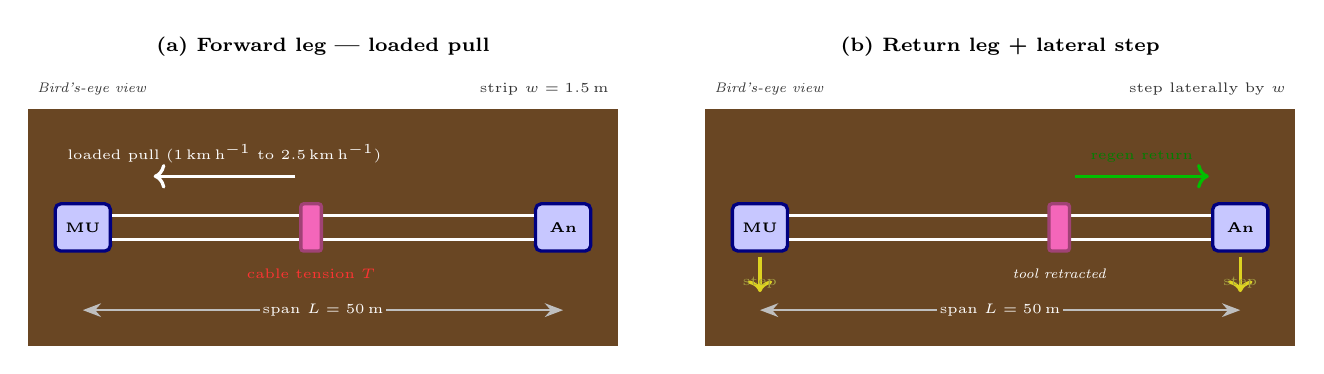
\begin{tikzpicture}[
    every node/.style={font=\scriptsize},
    mu/.style={draw=blue!50!black, very thick, fill=blue!22, rounded corners=2pt,
               minimum width=7mm, minimum height=6mm, align=center, font=\tiny\bfseries},
    anc/.style={draw=blue!50!black, very thick, fill=blue!22, rounded corners=2pt,
                minimum width=7mm, minimum height=6mm, align=center, font=\tiny\bfseries},
    impl/.style={draw=magenta!60!black, very thick, fill=magenta!60, rounded corners=1pt,
                 minimum width=2.6mm, minimum height=6mm, align=center,
                 font=\tiny\bfseries, text=white},
    field/.style={fill=brown!55!black},
    cable/.style={white, line width=1.2pt},
    dim/.style={<->, >=Stealth, gray!50!white, thick},
]

% =====================================================================
% PANEL A: Forward (loaded) leg
% =====================================================================
\begin{scope}[xshift=0cm]
% Panel title well above the field
\node[font=\scriptsize\bfseries, anchor=south] at (3.75,3.55) {(a) Forward leg --- loaded pull};

% Bird's-eye view label outside the field, above
\node[font=\tiny\itshape, gray!40!black, anchor=south west] at (0,3.05) {Bird's-eye view};
% Width tick label outside the field, above-left
\node[font=\tiny, gray!40!black, anchor=south east] at (7.5,3.05) {strip $w = \SI{1.5}{\meter}$};

% Field background
\fill[field] (0,0) rectangle (7.5,3);

% MU on left, Anchor on right
\node[mu] (mu1) at (0.7,1.5) {MU};
\node[anc] (an1) at (6.8,1.5) {An};

% Two parallel cables drawn straight horizontal across the field
\draw[cable] ($(mu1.east) + (0,0.15)$) -- ($(an1.west) + (0,0.15)$);
\draw[cable] ($(mu1.east) + (0,-0.15)$) -- ($(an1.west) + (0,-0.15)$);

% Implement carriage in the middle, riding on the cables
\node[impl] (im1) at (3.6,1.5) {};

% Motion arrow above the cables, pointing left (loaded toward MU)
\draw[->, very thick, white] (3.4,2.15) -- (1.6,2.15);
\node[white, font=\tiny, anchor=south] at (2.5,2.2) {loaded pull (\SIrange{1}{2.5}{\km\per\hour})};

% Cable tension annotation below the cables
\node[red!80!white, font=\tiny, anchor=north] at (3.6,1.1) {cable tension $T$};

% Span dimension at the very bottom of the field
\draw[dim] (mu1.south |- 0,0.45) -- (an1.south |- 0,0.45);
\node[white, font=\tiny, fill=brown!55!black, inner sep=1pt]
    at (3.75,0.45) {span $L = \SI{50}{\meter}$};
\end{scope}

% =====================================================================
% PANEL B: Return (unloaded) leg + lateral step
% =====================================================================
\begin{scope}[xshift=8.6cm]
\node[font=\scriptsize\bfseries, anchor=south] at (3.75,3.55) {(b) Return leg + lateral step};

\node[font=\tiny\itshape, gray!40!black, anchor=south west] at (0,3.05) {Bird's-eye view};
\node[font=\tiny, gray!40!black, anchor=south east] at (7.5,3.05) {step laterally by $w$};

\fill[field] (0,0) rectangle (7.5,3);

\node[mu] (mu2) at (0.7,1.5) {MU};
\node[anc] (an2) at (6.8,1.5) {An};

\draw[cable] ($(mu2.east) + (0,0.15)$) -- ($(an2.west) + (0,0.15)$);
\draw[cable] ($(mu2.east) + (0,-0.15)$) -- ($(an2.west) + (0,-0.15)$);

% Implement returning toward anchor (closer to right side)
\node[impl] (im2) at (4.5,1.5) {};

% Motion arrow above the cables, pointing right (unloaded back to anchor)
\draw[->, very thick, green!75!black] (4.7,2.15) -- (6.4,2.15);
\node[green!50!black, font=\tiny, anchor=south] at (5.55,2.2) {regen return};

% Tool retracted label, below the implement
\node[white, font=\tiny\itshape, anchor=north] at (4.5,1.1) {tool retracted};

% Lateral step arrows on both modules — pointing down (into the page, perpendicular to cable)
\draw[->, very thick, yellow!85!black] (mu2.south) ++(0,-0.05) -- ++(0,-0.45);
\node[yellow!60!black, font=\tiny, anchor=north] at (0.7,1.0) {step};
\draw[->, very thick, yellow!85!black] (an2.south) ++(0,-0.05) -- ++(0,-0.45);
\node[yellow!60!black, font=\tiny, anchor=north] at (6.8,1.0) {step};

% Span dimension at the very bottom of the field
\draw[dim] (mu2.south |- 0,0.45) -- (an2.south |- 0,0.45);
\node[white, font=\tiny, fill=brown!55!black, inner sep=1pt]
    at (3.75,0.45) {span $L = \SI{50}{\meter}$};
\end{scope}

\end{tikzpicture}
\caption{One round of the CableTract operating cycle, bird's-eye view. The two drawn lines are the working and return sides of the continuous cable loop (\gls{mu} drum $\to$ carriage $\to$ Anchor sheave $\to$ drum). \textbf{(a) Forward leg:} the Main Unit's winch reels in the working side, the implement carriage moves loaded toward the MU at \SIrange{1.5}{2.5}{\kilo\meter\per\hour}, the working tool engages the soil, and approximately the full draft $F_{\text{draft}}$ (plus loop pretension) is reacted at the Anchor. \textbf{(b) Return leg:} the tool retracts and the winch reverses, towing the carriage back along the loop at low tension; on sloped fields the four-quadrant drive recovers potential energy (\cref{sec:regen,sec:variant-norering}; the flat-field recovery is ${\approx}0$). After the return, the MU and the Anchor retract their ground screws, each step laterally by one strip width (\SI{1.5}{\meter}), and re-anchor; the cycle repeats on the next strip.}
\label{fig:f0c}
\end{figure}

\textbf{Cable topology.} The cable is a continuous loop: it leaves the \gls{mu} drum, runs to the carriage, continues to the redirect sheave on the Anchor, and returns to a second groove of the same drum. The two parallel lines drawn in \cref{fig:f0c} are the working and return sides of this loop. The winch therefore drives the carriage in \emph{both} directions --- loaded toward the \gls{mu} on the working side, and unloaded back toward the Anchor on the return side --- and the loop stays tensioned throughout, which is what makes four-quadrant (regenerative) operation on the return leg physically possible (\cref{sec:regen}). During the loaded pull the Anchor sheave reacts approximately the full draft plus the loop pretension.

One round of work proceeds as (\cref{fig:f0c}):

\begin{enumerate}[leftmargin=1.6em,itemsep=0.1em]
    \item The implement carriage starts at the Anchor end with the working tool engaged.
    \item The \gls{mu}'s winch reels in the working side of the loop. The carriage moves loaded toward the \gls{mu} at the operating speed (typically \SIrange{1.5}{2.5}{\kilo\meter\per\hour}).
    \item At the \gls{mu} end, the carriage tool retracts and the winch reverses, towing the carriage back to the Anchor end on the return side of the loop at low tension; on downhill return legs the four-quadrant drive recovers potential energy (\cref{sec:regen}).
    \item The \gls{mu} and Anchor retract their ground screws, each step laterally by one strip width, and re-set the screws (the anchoring cycle whose time and energy are bookkept in \cref{sec:anchoring-energy}).
    \item The cycle repeats on the next strip; after $\lceil \text{field depth}/\SI{50}{\meter}\rceil$ strip blocks, both modules reposition to the next block along their lanes.
\end{enumerate}

Typical numbers for the codesigned reference: span \SI{50}{\meter}, strip width \SI{1.5}{\meter}, carriage mass ${\approx}\SI{250}{\kilogram}$, operating speed \SIrange{1.5}{2.5}{\kilo\meter\per\hour}, setup time per round \SI{60}{\second}.

\subsection{Why an asymmetric architecture}\label{sec:asymmetry}

\begin{figure}[H]
\centering
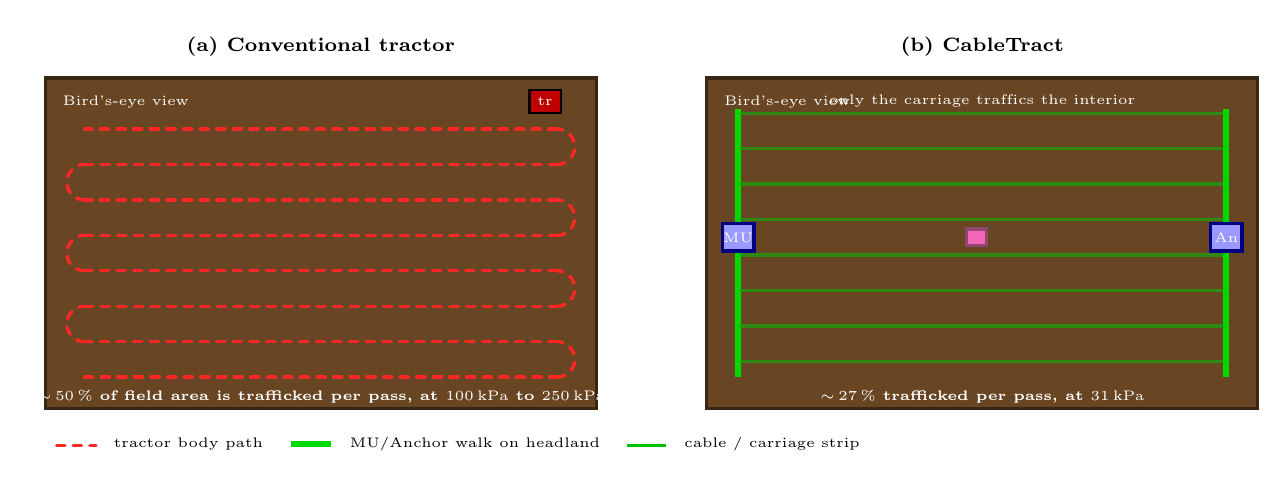
\begin{tikzpicture}[
    every node/.style={font=\tiny},
    field/.style={fill=brown!55!black, draw=brown!30!black, very thick},
    tractor/.style={red!85!white, very thick, dashed, line cap=round},
    cable/.style={green!75!black, very thick},
    ctcarriage/.style={green!85!black, line width=2.2pt},
    legend/.style={font=\tiny, anchor=west},
]

% =====================================================================
% PANEL A: Conventional tractor — snake path covering the whole field
% =====================================================================
\begin{scope}[xshift=0cm]
\node[font=\scriptsize\bfseries, anchor=south] at (3.5,4.35) {(a) Conventional tractor};
\fill[field] (0,0) rectangle (7,4.2);
\node[white, font=\tiny, anchor=north west] at (0.1,4.1) {Bird's-eye view};

% Snake / boustrophedon path covering the whole field
% 8 horizontal sweeps connected by U-turns
\foreach \i [evaluate=\i as \y using {0.4+0.45*\i}] in {0,1,...,7} {
    \ifodd\i
        \draw[tractor] (6.5,\y) -- (0.5,\y);
    \else
        \draw[tractor] (0.5,\y) -- (6.5,\y);
    \fi
}
% U-turns at the ends
\foreach \i in {0,2,4,6} {
    \pgfmathsetmacro{\ya}{0.4+0.45*\i}
    \draw[tractor] (6.5,\ya) arc (-90:90:0.225);
}
\foreach \i in {1,3,5} {
    \pgfmathsetmacro{\ya}{0.4+0.45*\i}
    \draw[tractor] (0.5,\ya) arc (270:90:0.225);
}

% Tractor icon at top-right indicating direction
\draw[fill=red!75!black, draw=black, thick]
    (6.15,3.75) rectangle (6.55,4.05);
\node[font=\tiny, white] at (6.35,3.9) {tr};

% Compacted area annotation
\node[white, font=\tiny\bfseries, align=center] at (3.5,0.15)
    {${\sim}\,50\,\%$ of field area is trafficked per pass, at \SIrange{100}{250}{\kilo\pascal}};
\end{scope}

% =====================================================================
% PANEL B: CableTract — straight headland edge path only
% =====================================================================
\begin{scope}[xshift=8.4cm]
\node[font=\scriptsize\bfseries, anchor=south] at (3.5,4.35) {(b) CableTract};
\fill[field] (0,0) rectangle (7,4.2);
\node[white, font=\tiny, anchor=north west] at (0.1,4.1) {Bird's-eye view};

% MU and Anchor walking along left and right headlands respectively
\draw[ctcarriage] (0.4,0.4) -- (0.4,3.8);
\draw[ctcarriage] (6.6,0.4) -- (6.6,3.8);

% Cable / strip indications across the field at sample positions
\foreach \y in {0.6,1.05,1.5,1.95,2.4,2.85,3.3,3.75} {
    \draw[cable, opacity=0.55] (0.4,\y) -- (6.6,\y);
}

% MU and Anchor module icons (current strip)
\draw[fill=blue!40, draw=blue!50!black, very thick] (0.2,2.0) rectangle (0.6,2.35);
\node[white, font=\tiny] at (0.4,2.175) {MU};
\draw[fill=blue!40, draw=blue!50!black, very thick] (6.4,2.0) rectangle (6.8,2.35);
\node[white, font=\tiny] at (6.6,2.175) {An};

% Implement carriage on the active cable
\draw[fill=magenta!60!white, draw=magenta!50!black, very thick]
    (3.3,2.07) rectangle (3.55,2.28);

% Annotation: only carriage rolls
\node[white, font=\tiny\bfseries, align=center] at (3.5,0.15)
    {${\sim}\,27\,\%$ trafficked per pass, at \SI{31}{\kilo\pascal}};
\node[white, font=\tiny, align=center] at (3.5,3.9)
    {only the carriage traffics the interior};
\end{scope}

% =====================================================================
% Caption-style legend below both panels
% =====================================================================
\node[legend, anchor=west] at (0,-0.45) {%
    \tikz{\draw[tractor] (0,0)--(0.5,0);} \, tractor body path
    \quad
    \tikz{\draw[ctcarriage] (0,0)--(0.5,0);} \, MU/Anchor walk on headland
    \quad
    \tikz{\draw[cable] (0,0)--(0.5,0);} \, cable / carriage strip};

\end{tikzpicture}
\caption{Why the lane-confined architecture wins on compaction --- and by how much. \textbf{(a)} A conventional tractor drives a boustrophedon (snake) path whose tyre tracks traffic ${\approx}50\,\%$ of the field area on every pass, at \SIrange{100}{250}{\kilo\pascal} contact pressure and ${\approx}\SI{4}{\tonne}$ of body mass. \textbf{(b)} CableTract keeps the Main Unit and the Anchor on lanes at the strip ends and runs a \SI{250}{\kilogram} carriage across the field; because the carriage must traverse \emph{every} \SI{1.5}{\meter} strip, its \SI{0.4}{\meter} of roller track traffics ${\approx}27\,\%$ of the field per pass --- roughly \emph{half} the tractor's trafficked area, at $4.6\times$ lower pressure. The field-integrated $p^2$-weighted exposure drops ${\approx}39\times$; see \cref{fig:f12} and \cref{sec:r-c1} for the quantitative model, and \cref{sec:related-ctf} for the comparison with controlled-traffic farming, which achieves \SIrange{15}{30}{\percent} lane fractions with conventional machinery.}
\label{fig:f0d}
\end{figure}

\Cref{fig:f0d} contrasts CableTract's headland-only coverage with a tractor's full-field boustrophedon path. Symmetric cable-traction systems (like the Orlando--Zoffoli patent~\cite{orlando2014patent}) need two winches, two batteries, two motor controllers, and two sets of high-power electronics. The asymmetric CableTract design moves all the power electronics into one module and lets the second module be a simple anchored drive. This roughly halves the \gls{bom} of the second module, halves its mass, and removes one of the two failure-prone winches.

The price of the asymmetry is that the cable reaction is one-sided. The Anchor must hold the entire horizontal draft against the soil. We address this with retractable ground screws (\cref{sec:anchor}) and quantify the per-auger requirement against \emph{two} published lateral-capacity references --- a realistic medium-dense fixed-head nominal and a deliberately pessimistic loose-sand bound --- so that every auger count is reported with its soil assumption made explicit.

\subsection{Co-designed implement library}\label{sec:codesign}

The single most impactful design choice in this paper is \textbf{building implements for CableTract instead of borrowing them from a tractor}. A conventional 8-row planter is built to survive the hitch loads of a multi-tonne tractor at \SI{9}{\kilo\meter\per\hour}; CableTract neither needs nor can usefully exploit those specifications. Two example entries in the co-designed library\footnote{Tabulated in \texttt{cabletract/data/asabe\_d497\_cabletract.csv} of the repository.} illustrate the two distinct kinds of gain. The \textbf{codesigned mower} (\SI{3}{\meter} rotary $\to$ \SI{1.5}{\meter}) gains \emph{genuine re-engineering}: its frame, freed from tractor hitch loads, cuts the D497 constant term $A$ by ${\approx}28\%$, so its \gls{p50} draft falls to $0.36\times$ the conventional entry --- more than the width halving alone would give. The \textbf{codesigned 4-row planter}, by contrast, halves per-pass draft (\SI{3.88}{\kilo\newton} $\to$ \SI{1.94}{\kilo\newton}) purely by halving the row count --- an \emph{operating-point} choice that is neutral in draft per unit area (half the rows cover half the area per pass). We are careful below to separate which library entries gain from genuine re-engineering and which from a lighter operating point, and which levers help \emph{energy per hectare} rather than only per-pass \emph{tension}.

The 10-implement codesigned library and the achieved draft reduction (\cref{tab:codesigned-library}):

\begin{table}[H]
\centering\small
\caption{Codesigned implement library, \gls{p50} draft reduction relative to the conventional \gls{asabe} D497.7~\cite{asabe-d497} entry it derives from. Medium-texture soil, samples from \cref{sec:soil-monte-carlo}.}\label{tab:codesigned-library}
\resizebox{\textwidth}{!}{%
\begin{tabular}{lllrlrr}
\toprule
Operation & Conventional implement & & Conv. P50 (N) & Codesigned implement & Codes. P50 (N) & Reduction \\
\midrule
primary tillage   & subsoiler 1-shank      &  & 10\,981 & narrow ripper 1-shank (\SI{15}{\centi\meter}) & 3\,022 & $0.28\times$ \\
primary tillage   & chisel plow 7-tool     &  & 14\,174 & narrow chisel 4-tool (\SI{12}{\centi\meter}) & 4\,219 & $0.30\times$ \\
secondary tillage & disk harrow \SI{2.5}{\meter} tandem & & 8\,428  & narrow disk \SI{1.5}{\meter} & 3\,231 & $0.38\times$ \\
secondary tillage & field cultivator 11 S-tine & & 3\,175 & narrow cultivator 6-tool & 1\,347 & $0.42\times$ \\
primary tillage   & sweep plow \SI{3}{\meter} & & 15\,412 & narrow sweep \SI{1.5}{\meter} & 5\,174 & $0.34\times$ \\
seeding           & row planter 8-row      &  & 3\,876  & codesigned planter 4-row & 1\,935 & $0.50\times$ \\
seeding           & grain drill 24-row     &  & 9\,302  & codesigned drill 12-row & 4\,650 & $0.50\times$ \\
weeding           & rotary hoe \SI{4}{\meter} &  & 2\,251 & codesigned rotary hoe \SI{2}{\meter} & 788 & $0.35\times$ \\
spraying          & boom sprayer           &  & 204     & codesigned sprayer \SI{1}{\meter}   & 143 & $0.70\times$ \\
mowing            & rotary mower \SI{3}{\meter} & & 1\,452 & codesigned mower \SI{1.5}{\meter} & 523 & $0.36\times$ \\
\midrule
\multicolumn{6}{r}{\textbf{Median reduction}} & $\boldsymbol{0.37\times}$ \\
\bottomrule
\end{tabular}%
}
\end{table}

\textbf{Median reduction across the 10 operations: $0.37\times$ (${\approx}\,63\%$ lower draft).} The reduction comes from three independent levers, each defensible from the \gls{asabe} D497.7 equation
\begin{equation}\label{eq:d497}
D \;=\; F_{\!\text{tex}} \,(A + B v + C v^{2})\, W \, T,
\end{equation}
where $D$ is draft (N), $v$ is field speed (\si{\kilo\meter\per\hour}), $W$ is the implement's natural width unit, $T$ is working depth, $F_{\!\text{tex}}$ is a soil-texture multiplier, and $(A,B,C)$ are machine-specific coefficients. The three levers are:

\begin{enumerate}[leftmargin=1.6em,itemsep=0.15em]
    \item \textbf{Width.} Halving $W$ halves \emph{per-pass} draft directly --- but worked area per pass halves with it, so this lever is \emph{energy-per-hectare neutral}. Its genuine value is to the \emph{tension} budget: per-pass draft is what the cable, the motor, and the anchor envelope must carry, and narrow widths are what keep all three small. The \SI{1.5}{\meter} strip is set by the widths at which the co-designed tools keep per-pass draft inside the 9-screw anchor envelope (\cref{sec:anchor}).
    \item \textbf{Speed.} The $B v + C v^{2}$ terms grow with speed. Operating at \SIrange{1.5}{2.5}{\kilo\meter\per\hour} instead of \SIrange{5}{9}{\kilo\meter\per\hour} cuts the narrow ripper's draft by ${\approx}31\%$ (\cref{fig:f5}) --- a genuine \emph{energy-per-hectare} gain, with the caveat that the D497 speed terms are here extrapolated below the standard's ${\sim}\SIrange{5}{13}{\kilo\meter\per\hour}$ calibration range (\cref{sec:soil-speed}), and that part of the speed-dependent draft performs soil-throw work whose agronomic role is operation-specific (\cref{tab:agronomic}).
    \item \textbf{Depth.} Working at $0.85\times$ the conventional depth drops $T$ by 15\,\% per pass; with the extra primary-tillage pass bookkept to compensate, the depth lever is \emph{energy-per-hectare negative} ($2\times0.85=1.7\times$) and is taken for the anchor and carriage load budgets, not for energy.
\end{enumerate}

In energy-per-hectare terms, therefore, the genuine levers are speed, the lighter frames (constant term $A$), and electric conversion; width and row count buy \emph{tension} margin, and depth costs energy but buys feasibility. \Cref{sec:r-c2} carries this decomposition into the headline claim.

\textbf{Accounting of the levers.} Most of the library's per-pass draft reduction comes from \emph{operating-point} choices rather than implement re-engineering, and we state this plainly. For the depth-dependent tillage tools (narrow ripper, chisel, sweep, cultivator, disk) the codesigned entries in \texttt{cabletract/data/asabe\_d497\_cabletract.csv} carry the \emph{same} D497.7 $(A,B,C)$ coefficients as the conventional implement they derive from; the per-pass reduction is obtained by running the same tool geometry shallower, slower, and on a narrower strip. This is physically real --- \cref{eq:d497} is linear in $W$ and $T$ and rises with $v$ --- but it carries an agronomic obligation: a shallow narrow pass is not interchangeable with a deep wide one for every tillage objective (a \SI{15}{\centi\meter} ripper pass does not fracture a deep plough pan the way a \SI{40}{\centi\meter} subsoiler pass does), which is why we bookkeep an extra primary-tillage pass and restrict the heaviest operations to favourable soil in \cref{sec:anchor}. The row-count halving for the planter and drill is throughput- and energy-per-area-neutral. Only the lighter tools (rotary hoe, mower, sprayer) gain a genuine reduction in the constant term $A$ from a frame freed of tractor hitch loads. We therefore present the $0.37\times$ median as the achieved \emph{per-pass draft ratio} at the codesigned operating point --- the quantity relevant to the cable-tension, motor and anchor budgets --- and not as an energy-per-hectare claim, which is governed by the separate lever accounting above. \Cref{tab:agronomic} states, per operation, where the reduction comes from and whether the codesigned pass is agronomically equivalent --- a design judgement to be confirmed by a prototype, not a measured result.

\begin{table}[H]
\centering\small
\caption{Agronomic-equivalence status of each co-designed operation. ``Source'' separates genuine implement re-engineering (a lighter frame lowers the constant term $A$) from operating-point choices (narrower $W$, slower $v$, shallower $T$, with D497 coefficients unchanged). Equivalence is a design judgement for a prototype to test.}\label{tab:agronomic}
\resizebox{\textwidth}{!}{%
\begin{tabular}{lll}
\toprule
Operation (conventional $\to$ codesigned) & Draft-reduction source & Agronomic-equivalence status \\
\midrule
subsoiler $\to$ narrow ripper (\SI{15}{\centi\meter})       & depth + speed (coeffs unchanged) & \emph{Not} equivalent for deep pan; needs 2 passes / favourable soil \\
chisel 7-tool $\to$ narrow chisel 4-tool                    & depth + speed + tool count       & Approx.\ equivalent with an extra pass \\
sweep \SI{3}{\meter} $\to$ narrow sweep \SI{1.5}{\meter}     & width + depth (coeffs unchanged) & Approx.\ equivalent (more strips) \\
disk \SI{2.5}{\meter} $\to$ narrow disk \SI{1.5}{\meter}     & width + depth + speed (coeffs unchanged) & Penetration, soil throw and residue cutting at \SI{2}{\kilo\meter\per\hour} unverified \\
cultivator 11-tine $\to$ 6-tool                             & width + tool count               & Likely equivalent \\
planter 8-row $\to$ 4-row                                   & row count (area-neutral)         & Equivalent (twice the strips) \\
grain drill 24-row $\to$ 12-row                             & row count (area-neutral)         & Equivalent (twice the strips) \\
rotary hoe \SI{4}{\meter} $\to$ \SI{2}{\meter}              & width + lighter frame ($A$, $-30\%$) & \emph{Not} equivalent at cable speeds --- blind-weeding efficacy relies on \SIrange{8}{16}{\kilo\meter\per\hour} tip flick; needs a powered rotor or an inter-row hoe substitute \\
boom sprayer $\to$ \SI{1}{\meter} sprayer                   & lighter frame ($A$, $-30\%$; width \SI{1}{\meter} in both entries) & Equivalent (pump power budgeted separately, \cref{sec:carriage-power}) \\
rotary mower \SI{3}{\meter} $\to$ \SI{1.5}{\meter}          & width + lighter frame ($A$, $-28\%$) & Equivalent \emph{as draft}; cutting power budgeted separately (\cref{sec:carriage-power}) \\
\bottomrule
\end{tabular}%
}
\end{table}

The price of the codesigned library is that the farmer cannot take a CableTract to a neighbour's field and hook up the neighbour's plough. CableTract is sold as a \emph{system} --- Main Unit + Anchor + carriage + implements --- not as a generic cable robot that accepts off-the-shelf tools. This is the same business model as FarmDroid, ecoRobotix, and Na\"io Technologies.

% ====================================================================
\section{Research Questions}\label{sec:rqs}
% ====================================================================

We organise the analysis around four claims and seven research questions. The four claims are the headline assertions the paper defends with code-traceable numbers; the seven research questions decompose each claim into the operational regime, the physical mechanism, and the binding constraint.

\paragraph{C1 --- Compaction.} CableTract reduces the trafficked field area by at least 40\,\% \emph{and} the field-integrated $p^2$-weighted soil-stress exposure by at least $20\times$ compared with an \SI{80}{hp} \gls{wd} diesel tractor on the same field, because the field interior is trafficked only by the lightweight carriage's low-pressure rollers while the \gls{mu} and Anchor stay on fixed lanes.

\paragraph{C2 --- Energy.} With a co-designed implement library, the anchoring cycle charged explicitly, and regenerative braking on the return leg (the default design), CableTract operates at ${\approx}\SI{1.23}{\kWh\per\decare}$ (${\approx}\SI{12.3}{\kWh\per\hectare}$) of delivered electrical energy --- below the diesel comparator's estimated \emph{drawbar} work by a factor of ${\sim}2.9$ and below its \emph{primary fuel} energy by ${\sim}10\times$ --- driven by (i) the absence of dead-weight transport, (ii) the slow-speed draft reduction, (iii) lighter implement frames, and (iv) electric rather than thermal conversion. (This is a mixed accounting basis, conservative in the comparator's favour: CableTract's own drawbar output is smaller than its delivered electricity by its drivetrain efficiency.)

\paragraph{C3 --- Off-grid.} Under a seasonal 170-day duty cycle with \SI{15}{\meter\squared} of \gls{pv} and a \SI{9}{\kWh} battery, annual grid dependence is below \SI{100}{\hour\per\year} at the highest-irradiance bundled site (Konya, \SI{58}{\hour}), and \SIrange{150}{282}{\hour\per\year} at the other five (Des Moines, Palencia, São Paulo, Ludhiana, Beauce) --- i.e.\ \SIrange{94}{98}{\percent} of in-season energy is harvested on-board everywhere, full autonomy is site-conditional, and no bundled site is categorically infeasible. The off-grid claim is \emph{climate-conditional}, not categorical.

\paragraph{C4 --- Economics and life-cycle CO\textsubscript{2}.} The replacement-frame economics are \emph{scale-conditional}: with the carriage costed, the implement set carried symmetrically on both sides, and the cable-replacement line included, \gls{npv} versus a used diesel tractor at 8\,\% is ${\approx}\SI{-1.7}{\kilo\EUR}$ at \SI{25}{\hectare\per\year} (cost-neutral within parameter uncertainty), positive above ${\sim}\SI{40}{\hectare\per\year}$ at all three tested discount rates, and \SI{+9.1}{\kilo\EUR} at \SI{100}{\hectare\per\year}. Life-cycle CO\textsubscript{2} is \SI{17.0}{\kilogram\per\hectare\per\year} versus 32.5 for diesel --- a $1.9\times$ improvement that does not depend on grid decarbonisation.

\medskip
The research questions:

\begin{description}[leftmargin=2.0em,style=nextline,itemsep=0.25em]
    \item[\gls{rq}1] What is the compacted-area reduction and contact-energy reduction across rectangle, L-shape, and irregular-concave field classes?
    \item[\gls{rq}2] What energy per decare does the codesigned reference achieve, and how does it decompose between mechanical work, drivetrain losses, and dead-weight motion?
    \item[\gls{rq}3] Under which combinations of annual \gls{ghi}, panel area, and battery capacity is the system off-grid capable?
    \item[\gls{rq}4] For which operation classes is the architecture most favourable, and where does the ground-screw anchor envelope bind?
    \item[\gls{rq}5] How do polygon shape and size erode the throughput on real fields?
    \item[\gls{rq}6] Is the codesigned reference Pareto-optimal on (CAPEX $\times$ throughput $\times$ payback $\times$ energy intensity), or does it leave headroom?
    \item[\gls{rq}7] Across the (annual \gls{ghi} $\times$ farm size) plane, where is CableTract \gls{npv}-positive against diesel, and where does the off-grid feasibility envelope bind first?
\end{description}

% ====================================================================
\section{Methods}\label{sec:methods}
% ====================================================================

\subsection{Modelling philosophy}\label{sec:philosophy}

The analysis is parametric and designed to expose its assumptions. Every parameter has units, every default value has a citation in a bundled data file, and every claim in \cref{sec:results} has a per-figure CSV companion with the underlying numbers.\footnote{Full source and data: \cabletractrepo} We do not attempt high-fidelity soil-tool dynamics, full closed-loop control simulation, or finite-element cable modelling. We use first-principles work-energy balances, the standard \gls{asabe} D497.7 implement-draft equation, an hourly \gls{tmy}-based PV+battery simulator, a static contact-pressure compaction model, a discounted-cash-flow economics engine, and global Sobol sensitivity over 20 inputs. This is the appropriate fidelity for an early-stage feasibility study.

Every higher-level analysis is composed on top of one atomic computation that takes a parameter set and returns a result record. The energy simulator (\cref{sec:energy}), the global sensitivity decomposition (\cref{sec:sobol}), the architectural variants (\cref{sec:ml}), and the operating envelope (\cref{sec:envelope}) are all callers of this same routine. Every figure is therefore re-derived from a single physics-and-economics chain rather than from parallel approximations that drift apart.

\subsection{Codesigned reference parameter set}\label{sec:codesigned-ref}

The codesigned reference is the single system the rest of the paper analyses. It is \emph{the} baseline: there is no other parameter set we report headline numbers on, so every result in \cref{sec:results} can be traced back to the values in \cref{tab:codesigned-params}, which lists each entry together with a one-line engineering justification.

\begin{table}[H]
\centering\small
\caption{Codesigned reference parameter set. Used unchanged in every figure, table, and headline number in the paper.}\label{tab:codesigned-params}
\begin{tabularx}{\textwidth}{lrX}
\toprule
Parameter & Value & Notes \\
\midrule
span (\si{\meter}) & 50 & Anchor-to-Main-Unit cable distance \\
strip width (\si{\meter}) & 1.5 & Matches the codesigned implement library \\
implement + cable transport load (N) & 600 & Carriage tool + cable drag carried along the span ($F_i$ in \cref{eq:pass}); the carriage \emph{structural} mass is ${\approx}\SI{250}{\kilogram}$ and enters the compaction model (\cref{sec:compaction}) \\
draft load (N) & 1\,800 & Representative \gls{p50} for the medium-load operational calendar; the full 10-implement library median is \SI{2479}{\newton} (\cref{sec:soil-codesigned}), with heavy primary tillage higher \\
system repositioning load (N) & 2\,200 & Rolling-resistance force as the ${\approx}\SI{2}{\tonne}$ MU\,+\,Anchor step between strips ($F_s$ in \cref{eq:pass}); a force, not a mass \\
lateral travel per round (m) & 2.0 & Strip width (\SI{1.5}{\meter}) plus \SI{0.5}{\meter} manoeuvre allowance ($d_s$ in \cref{eq:pass}) \\
drivetrain efficiency (effective) & 0.518 & One-way chain 0.50 (6 components, \cref{sec:drivetrain}) $+\,{\approx}3.5\%$ four-quadrant recovery (slope-averaged; ${\approx}0$ on flat) \\
anchoring energy (\si{\Wh} per round) & 25.3 & Insert + retract 9 Anchor + 4 MU ground screws, \SI{1.0}{\meter} at \SI{90}{\newton\meter} final torque (\cref{sec:anchoring-energy}) \\
\gls{pv} area (\si{\meter\squared}) & 15 & Mono-Si flat plate, deployable \\
wind generator (W) & 100 & Typical harvested power; a \SI{600}{\watt}-rated helix \gls{vawt} ($C_p = 0.30$) that reaches nameplate only near \SI{12}{\meter\per\second} (\cref{sec:pvwindbat}) \\
setup time per round (\si{\second}) & 60 & Ground-screw cycle + cable re-tension + carriage hookup (\cref{sec:anchoring-energy}) \\
battery (\si{\kWh}) & 9 & Li-ion, 96/96\,\% charge/discharge eff. \\
operating window (\si{\hour\per day}) & 10 & Daily total work window (the battery simulation's \SI{6}{\hour} solar window is a separate quantity, \cref{sec:pvwindbat}) \\
operating days/yr & 170 & Contiguous seasonal calendar (hemisphere-aware, \cref{sec:synth}) \\
diesel reference fuel (\si{\litre\per\decare}) & 1.2 & Mid-range field operation (\SI{12}{\litre\per\hectare})~\cite{siemens1999machinery,asabe-d497} \\
diesel price (\si{\EUR\per\litre}) & 1.40 & EU 2024 agricultural diesel \\
capex CableTract (\si{\EUR}) & 38\,670 & Machine incl.\ carriage; itemised in \cref{sec:economics}; implement set carried symmetrically \\
project horizon (\si{\year}) & 15 & Typical design life for the vehicle class \\
discount rate (\%) & 8 & Financing-rate proxy for the opportunity cost of capital; 5 and 12\,\% also reported \\
\bottomrule
\end{tabularx}
\end{table}

\subsection{Pass model}\label{sec:pass-model}

For one round of work, the delivered electrical energy is
\begin{equation}\label{eq:pass}
E_{\text{round}} \;=\; \frac{F_d\,L \;+\; F_t\,L \;+\; F_s\,d_s}{\eta_{\text{drivetrain}}} \;+\; E_{\text{anchor}},
\end{equation}
where $F_d$ is the implement draft (N), $F_t$ the equivalent horizontal transport resistance of the carriage and cable (rolling resistance of the carriage rollers plus cable drag, \SI{600}{\newton}), $F_s$ the system-repositioning force (N), $L$ the cable span (m), $d_s$ the lateral repositioning distance per round (\SI{2.0}{\meter}, \cref{tab:codesigned-params}), and $E_{\text{anchor}}$ the anchoring-cycle energy of \cref{sec:anchoring-energy}. For the codesigned reference the mechanical breakdown is $F_d L = \SI{90}{\kilo\joule}$ (72\,\% of mechanical work), $F_t L = \SI{30}{\kilo\joule}$ (24\,\%), and $F_s d_s = \SI{4.4}{\kilo\joule}$ (4\,\%); after the drivetrain (\SI{66.7}{\Wh}) and the anchoring cycle (\SI{25.3}{\Wh}, 27\,\% of the electrical total), one round delivers \SI{92.0}{\Wh}, giving the \SI{1227}{\Wh\per\decare} headline at 13.3 rounds per decare. The dead-weight saving relative to a tractor is visible in the $F_s d_s$ term: the module-repositioning work is paid once per strip rather than over the whole field. Note that $F_t$ is a dissipative resistance, so $F_t L$ is genuine work, not a conservative over-estimate.

\subsection{Cable mechanics, drivetrain, anchor}\label{sec:physics}

The cable mechanics and drivetrain model are verified against 22 analytic invariants (sag monotonicity, Hooke's law in the elastic regime, energy conservation on the regen leg, and others).\footnote{Test suite: \texttt{tests/test\_physics.py} in the repository.}

\subsubsection{Decomposed drivetrain efficiency}\label{sec:drivetrain}

A lumped winch efficiency $\eta_w \approx 0.5$ is the most common single-parameter shortcut in agricultural-electrification work. It collapses six independent loss mechanisms --- motor copper losses, inverter switching losses, gearbox friction, drum tension losses, pulley redirect losses, cable elongation hysteresis --- into one number, which a global sensitivity analysis (\cref{sec:sobol}) would then assign almost all of the variance to. The chain we use in this paper is the explicit product of those six components, each independently sourced from a datasheet or a published engineering standard:

\begin{equation}\label{eq:eta-chain}
\eta_{\text{drivetrain}} \;=\; \eta_{\text{motor}} \,\eta_{\text{ctrl}}\, \eta_{\text{gearbox}} \,\eta_{\text{drum}}\, \eta_{\text{pulley}}\, \eta_{\text{cable}}.
\end{equation}

Two presets are bundled (\cref{tab:eta-decomposition}); the ``baseline'' \emph{one-way} product matches the lumped 0.5 by construction, and ``premium'' recovers ${\approx}74\%$. The component decomposition is what justifies the $[0.35, 0.65]$ band over which the global sensitivity analysis of \cref{sec:sobol} samples the (single, lumped) drivetrain-efficiency parameter --- the chain shows the band's endpoints correspond to a low-cost and a best-of-class build rather than to an undefended fudge factor. (The Sobol problem itself samples the lumped efficiency, not the six components separately.)

This one-way chain governs \emph{motor sizing} (the peak loaded pull, \cref{sec:motor}). The \emph{energy budget} uses a slightly higher effective efficiency, because the default four-quadrant drive recovers a \emph{modest}, slope-driven amount of energy on the unloaded return leg (\cref{eq:regen}). We are deliberately conservative about its size. The draft work itself --- the dominant ${\sim}90\,\si{\kilo\joule}$ per pass --- is dissipated irreversibly in cutting soil and \emph{cannot} be regenerated; the carriage kinetic energy at \SI{2}{\kilo\meter\per\hour} is only ${\sim}\SI{40}{\joule}$ (negligible); and on a perfectly flat field the recovery is zero. We therefore credit only ${\approx}3.5\%$ as a \emph{slope-averaged} figure over the gently-undulating fields of the target regions, lifting the effective drivetrain efficiency from the one-way 0.50 to ${\approx}0.518$ --- \emph{not} the large ``half the round is unloaded'' recovery a naive argument would suggest, and \emph{zero} on flat ground. This gives a headline \SI{1227}{\Wh\per\decare}, against a flat-field / no-regen value of \SI{1259}{\Wh\per\decare} (the unidirectional drivetrain, \cref{sec:variant-norering}). The four-quadrant drive is a modest hardware premium (${\approx}\SI{300}{\EUR}$, folded into the Main Unit) and is standard equipment primarily for smooth depth-control torque and slope recovery, not as a flat-field energy lever.

\begin{table}[H]
\centering\small
\caption{Decomposed drivetrain efficiency. Baseline product reproduces the lumped 0.5; premium recovers 0.74.}\label{tab:eta-decomposition}
\begin{tabularx}{\textwidth}{Xrrl}
\toprule
Component & Baseline (low-cost) & Premium (best-of-class) & Source \\
\midrule
\gls{pmsm} motor              & 0.85 & 0.93 & \cite{asabe-ep496} \\
Three-phase inverter           & 0.92 & 0.96 & \cite{asabe-ep496} \\
2-stage planetary gearbox      & 0.88 & 0.95 & drive-vendor data \\
Drum capstan + bending         & 0.88 & 0.95 & \cite{feyrer2015wireropes} \\
Redirect sheave block          & 0.90 & 0.95 & \cite{feyrer2015wireropes} \\
Cable cyclic loss              & 0.92 & 0.97 & Marlow Excel D12 datasheet \\
\midrule
\textbf{Product}               & \textbf{0.50} & \textbf{0.74} & --- \\
\bottomrule
\end{tabularx}
\end{table}

\subsubsection{Catenary sag}\label{sec:catenary}

The first geometric requirement for any cable-based field robot is that the cable must not sag into the soil. If midspan sag exceeds the implement-attachment height, the geometry breaks before any draft, energy, or economics question can be asked. \Cref{fig:f1} resolves this with a closed-form bound: it computes the minimum horizontal tension required to keep midspan sag below the depth-control clearance budget, as a function of cable material, span, and self-weight.

A perfectly flexible cable of self-weight $w$ (\si{\newton\per\meter}) hung between two supports a horizontal distance $L$ apart at horizontal tension $T_h$ takes the catenary shape~\cite{irvine1981cables}
\begin{equation}\label{eq:catenary}
y(x) \;=\; a\bigl(\cosh(x/a)-1\bigr), \qquad a \;=\; T_h / w,
\end{equation}
with midspan sag
\begin{equation}\label{eq:sag-exact}
s \;=\; a\!\left(\cosh\!\left(\frac{L}{2a}\right) - 1\right).
\end{equation}
For $w L / (2 T_h) < 0.3$ the parabolic limit
\begin{equation}\label{eq:sag-parabolic}
s \;\approx\; \frac{w L^{2}}{8 T_h}
\end{equation}
is accurate to 1\,\%. Both forms are computed and cross-checked at every operating point.

\Cref{fig:f1} sweeps horizontal cable tension from \SI{0.5}{\kilo\newton} to \SI{25}{\kilo\newton} for steel 6$\times$19 \gls{iwrc}, Dyneema SK78 12-strand, and Spectra 1000 fibre rope (all \SI{8}{\milli\meter} nominal) at three spans $L \in \{50, 75, 100\}\,\si{\meter}$.\footnote{Mechanical properties from manufacturer datasheets, tabulated in \texttt{cabletract/data/cable\_props.csv}.}

\begin{figure}[H]
\centering

\includegraphics[width=0.85\linewidth]{F1_cable_sag}
\caption{Catenary sag versus horizontal cable tension for three rope materials at three spans. \emph{Tilling depth is set by the carriage's own depth wheel, not by cable sag} (\cref{sec:tension-balance}); the cable's only geometric job is to stay clear of the soil/crop. For a cable support height of ${\approx}\SI{0.8}{\meter}$ and a ground-clearance budget of ${\sim}\SI{0.3}{\meter}$ (a sag limit of ${\sim}\SI{0.5}{\meter}$), \SI{8}{\milli\meter} Dyneema (self-weight \SI{0.046}{\kilogram\per\meter}) needs only ${\approx}\SI{0.3}{\kilo\newton}$ pretension at the \SI{50}{\meter} reference span and ${\approx}\SI{1.1}{\kilo\newton}$ at \SI{100}{\meter} (parabolic limit $T\approx wL^2/8s$). This modest sag-floor pretension is below the implement draft for all but the lightest operations, so the Anchor reaction is governed by the \emph{draft} (\cref{sec:anchor}), not by sag. (A much tighter $\pm\SI{2}{\centi\meter}$ tolerance, were it required of the cable, would demand ${\approx}\SI{7}{\kilo\newton}$ at \SI{50}{\meter} --- but that tolerance belongs to the carriage's depth control, not to the cable.) Steel needs ${\sim}5\times$ more tension for the same clearance because of its ${\sim}5\times$ higher self-weight, which is why CableTract uses synthetic rope.}
\label{fig:f1}
\end{figure}

\textbf{What this gives the rest of the paper.} \Cref{fig:f1} narrows the design choice to synthetic rope and quantifies the minimum working tension as a function of span. CableTract uses \SI{8}{\milli\meter} Dyneema throughout. The minimum-tension number flows into \cref{sec:tension-balance} (which side of the draft-bound vs sag-bound regime are we in?) and into \cref{sec:anchor} (the ground-screw capacity must absorb the horizontal tension we just selected).

\subsubsection{Tension balance and operating regime}\label{sec:tension-balance}

The implement carriage's own depth-control mechanism --- not the cable --- sets tilling depth. The cable transmits the horizontal draft $F_d$ and stays clear of the soil. Two regimes arise:

\begin{itemize}[leftmargin=1.6em,itemsep=0.15em]
    \item \textbf{Draft-bound:} $F_d$ is large enough that the resulting horizontal tension keeps midspan sag below the clearance budget $h_p - c_{\min}$. Horizontal tension equals $F_d$, anchor sees ${\approx}F_d$.
    \item \textbf{Sag-bound:} $F_d$ is too small to keep the cable taut against its own weight. The Main Unit over-tensions to $T_{\text{sag,min}}$. The anchor sees this larger tension.
\end{itemize}

The tension-balance solver detects which regime applies at each operating point and reports the tensions seen by both ends of the cable. \Cref{fig:f2} sweeps draft from \SI{0.2}{\kilo\newton} to \SI{16}{\kilo\newton} at \SI{8}{\milli\meter} Dyneema, span \SI{50}{\meter}, $h_p = \SI{1.5}{\meter}$, with the per-auger Anchor capacity bands overlaid.

\subsubsection{Anchor reaction envelope}\label{sec:anchor}

The asymmetric architecture of \cref{sec:asymmetry} only works if the lighter Anchor module can geotechnically resist the cable reaction. A mass-anchored solution would force the Anchor to weigh as much as a small tractor, which would defeat the architecture's selling point. We therefore replace mass anchoring with helical screw piles and quantify how many augers are required at each draft level. This is the load-bearing question behind the ``CableTract is mechanically possible'' claim.

The literature on lateral capacity of helical anchors spans nearly two orders of magnitude depending on soil density, shaft fixity, embedment, and the chosen serviceability limit~\cite{perko2009helical}, so we anchor the analysis between a realistic nominal and a deliberately pessimistic bound rather than picking one number. The \textbf{Magnum Piering 2024 design tables}~\cite{magnum2024fixed} report allowable lateral capacities of \SIrange{14}{20}{\kilo\newton} per small fixed-head helical pile in medium-dense sand (SPT $N \approx 10$--$30$) at a predicted \SI{0.5}{inch} ground-surface deflection (the datasheet's implementation of the IBC2021 allowable-capacity rule), and the industry-standard CHANCE Technical Design Manual~\cite{chance2024manual} brackets the same range. As our \emph{nominal} design basis we adopt a heavily conservative downscale of this --- \SI{2}{\kilo\newton} per screw (a $7$--$10\times$ reduction on the reported fixed-head values), at a working safety factor of 1.15 --- which corresponds to the medium-dense, frame-coupled (fixed-head) conditions a real installer would target. As a \emph{worst-case stress bound} we additionally carry \SI{400}{\newton} per screw, our per-pile reading of the 4-pile group raft tests of \textbf{Qureshi et al.\ (2024)}~\cite{khand2024helical} for short piles in \emph{loose} sand at strict deflection thresholds with free-head boundary conditions; we flag explicitly that this number is extracted from a 1g model-scale experiment, so it is used only as a pessimistic ordering bound, not as a field-calibrated capacity. Reporting both makes the soil assumption behind every screw count explicit --- and \cref{sec:v-s7} now \emph{derives} both ends of this bracket from a single internal $p$--$y$ model of the installed \SI{1.0}{\meter} ground screw: the free-head loose-sand working nominal comes out at \SI{0.37}{\kilo\newton} (reproducing the literature bound) and the frame-coupled fixed-head working values at \SIrange{1.9}{2.6}{\kilo\newton} (reproducing the \SI{2}{\kilo\newton} nominal). The codesigned 9-screw Anchor is sized so that even at the \SI{400}{\newton} worst-case bound it anchors the codesigned reference draft (P90 \SI{3.0}{\kilo\newton}, 9 screws); at the \SI{2}{\kilo\newton} nominal those same 9 screws carry the entire codesigned library --- and most conventional implements --- with a $4$--$5\times$ margin on screw count. We do not lean on the worst case to make the design work; we use it to show how much pessimism the design tolerates. The 9-screw capacity lines plotted in \cref{fig:f2,fig:f4} are \emph{nominal} ($9\times$ per-screw, i.e.\ \SI{3.6}{\kilo\newton} on the loose-sand bound and \SI{18}{\kilo\newton} on the Magnum nominal); the screw \emph{counts} we quote already apply the 1.15 working safety factor, $n = \lceil 1.15\,T / c \rceil$, so they are allowable-capacity counts, not nominal. Two load-path caveats bound this check: the cable enters at the sheave ${\approx}\SI{1}{\meter}$ above grade, so the screw group also carries an overturning couple (${\approx}\SIrange{3}{7}{\kilo\newton\meter}$ at P90-to-sweep loads) resolved as push--pull axial loads across the $3\times3$ cluster --- helix uplift capacity, not only lateral shear, must cover the tension row; and the \gls{mu} side, self-anchored by 4 screws plus ${\approx}\SI{14}{\kilo\newton}$ of module weight on its wheels ($\mu \approx 0.5$ gives ${\approx}\SI{7}{\kilo\newton}$ of friction alone), sees the same cable tension and is checked by the same envelope with its weight-friction share included. Both are screening checks; the moment-and-uplift group case is listed as an open analysis in \cref{sec:analytical-limitations}.

\begin{figure}[H]
\centering

\includegraphics[width=0.85\linewidth]{F2_anchor_envelope}
\caption{Anchor reaction envelope plotted against \emph{two} per-screw lateral capacity references that span the published range. \textbf{Dashed red bands (Qureshi et al.\ 2024~\cite{khand2024helical})}: \SI{400}{\newton} per short pile in \emph{loose} sand, free-head, strict deflection limit (the per-pile interpretation of the 4-pile raft tests in that paper) --- the worst-case bound. \textbf{Solid blue bands (Magnum Piering 2024~\cite{magnum2024fixed}, with~\cite{chance2024manual} as a corroborating manual reference)}: \SI{2}{\kilo\newton} per screw, a conservative downscale of the \SIrange{14}{20}{\kilo\newton} fixed-head capacity reported for medium-dense sand at a predicted \SI{0.5}{inch} deflection --- the realistic engineering nominal. The working safety factor is 1.15 in both envelope families. On the \SI{2}{\kilo\newton} nominal the codesigned reference (P50 \SI{1.8}{\kilo\newton}, P90 \SI{3.0}{\kilo\newton}) needs only 2 screws, so the installed 9-screw Anchor over-provisions by ${\sim}4.5\times$; on the \SI{400}{\newton} worst-case bound the same reference needs 6 (P50) and 9 (P90) screws, which is what sets the 9-screw count. A conventional implement library at \SIrange{8}{15.4}{\kilo\newton} (disk harrow to sweep plow) would require 25--45 screws on the loose-sand bound but only 5--9 on the medium-dense nominal. The codesigned library is what keeps the Anchor feasible \emph{even in worst-case soil}; in typical soil the same Anchor carries it with comfortable margin.}
\label{fig:f2}
\end{figure}

\textbf{Findings.} Working from the per-implement P50/P90 numbers in \cref{fig:f4}:
\begin{itemize}[leftmargin=1.6em,itemsep=0.15em]
    \item \textbf{Light codesigned operations are loose-sand feasible.} On the conservative Qureshi envelope, the 9-auger Anchor handles the codesigned cultivator (\SI{1.4}{\kilo\newton} P50, 5 augers required), planter (\SI{1.9}{\kilo\newton}, 6), rotary hoe (\SI{0.8}{\kilo\newton}, 3), sprayer (\SI{0.14}{\kilo\newton}, 1), and mower (\SI{0.5}{\kilo\newton}, 2) with margin. The narrow ripper at its P50 of \SI{3.0}{\kilo\newton} (8.6 augers) is the marginal case --- it sits at exactly the design value, and its P90 of \SI{3.8}{\kilo\newton} pushes 11 augers, just outside the installed envelope.
    \item \textbf{Heavy codesigned primary tillage is loose-sand restricted.} Four codesigned operations --- narrow sweep (\SI{5.2}{\kilo\newton} P50), narrow chisel (\SI{4.2}{\kilo\newton}), narrow disk (\SI{3.2}{\kilo\newton}), and codesign drill (\SI{4.6}{\kilo\newton}) --- exceed the 9-auger count at the \SI{400}{\newton} worst-case bound and would require \textbf{10--15 augers} at their P50 in loose sand. These four implements are restricted to the medium-dense nominal in the present design.
    \item \textbf{All codesigned operations are medium-dense feasible.} On the \SI{2}{\kilo\newton} nominal, the worst codesigned case (narrow sweep P90 \SI{7.25}{\kilo\newton}) requires \textbf{5 augers} --- the entire codesigned library fits inside the 9-auger Anchor with margin. The same 9-auger Anchor would also hold the heaviest \emph{conventional} implements (chisel plow \SI{14.2}{\kilo\newton} P50, sweep plow \SI{15.4}{\kilo\newton} P50 --- both 9 augers) at the design ceiling.
\end{itemize}

The reading of the physics chapter is therefore that the 9-auger Anchor is sized for the medium-dense soil regime, in which it carries the entire codesigned library with comfortable margin and is competitive even with conventional implements. In the worst-case loose-sand regime, the same Anchor is restricted to the lighter half of the codesigned library (cultivator, planter, rotary hoe, sprayer, mower, and the narrow ripper at its P50). The codesigned library is therefore not a worst-case geotechnical fix --- it is the design choice that simultaneously makes the energy budget work, the motor sizing work, and the medium-dense-soil anchor envelope work for the entire operation calendar. In loose-sand sites, the operating envelope shrinks to the lighter half of the library, and heavy primary tillage either waits for soil moisture conditions that improve fixity or is performed by a conventional implement on the same site.

The two-reference bracket above is deliberately agnostic about which per-screw capacity is ``correct''. \Cref{sec:v-s7} closes that gap with a nonlinear $p$--$y$ Winkler model of the \emph{installed} \SI{1.0}{\meter} ground-screw geometry, which derives working nominals of \SI{0.37}{\kilo\newton} (loose sand, free-head --- essentially reproducing the \SI{400}{\newton} literature bound) and \SIrange{1.9}{2.6}{\kilo\newton} (frame-coupled fixed-head --- reproducing the \SI{2}{\kilo\newton} nominal). The practical reading: with the screws rigidly coupled to the Anchor frame the 9-screw cluster carries the codesigned P90 with ${\gtrsim}5\times$ margin, while under the pessimistic free-head loose-sand reading the same cluster sits \emph{at} its envelope at the P90 (10 screws required at the derived \SI{374}{\newton} nominal vs 9 installed) --- so in loose sand the frame coupling, not redundancy, is what the design leans on. The screws are set once per round, in parallel, and their time and energy cost is charged in \cref{sec:anchoring-energy}.

\subsubsection{Peak vs continuous motor power}\label{sec:motor}

Day-averaged power numbers are convenient for energy budgets but misleading for motor sizing. A real motor must absorb the peak load --- start-up, loaded acceleration, transient draft spikes from the implement entering harder soil --- and the BOM cost of the motor, inverter, and cooling sits on that peak rather than on the average. We therefore separate the two.

Motor sizing is governed by the peak load, not the day-averaged power. We separate the two as
\begin{equation}\label{eq:power}
P_{\text{cont}} \;=\; \frac{F_{\text{cont}}\, v_{\text{cont}}}{\eta_{\text{drivetrain}}}, \qquad
P_{\text{peak}} \;=\; \frac{F_{\text{peak}}\, v_{\text{peak}}}{\eta_{\text{drivetrain}}},
\end{equation}
evaluated at the sizing speed $v_{\text{cont}} = v_{\text{peak}} = \SI{0.50}{\meter\per\second}$ (\SI{1.8}{\kilo\meter\per\hour}) used throughout \cref{fig:f3}. For the reference-calendar loads (\SI{1.8}{\kilo\newton} P50 / \SI{3.0}{\kilo\newton} P90) the baseline chain requires \SI{1.80}{\kilo\watt} continuous / \SI{3.00}{\kilo\watt} peak, and the codesigned reference selects a \textbf{\SI{2.0}{\kilo\watt} continuous / \SI{3.0}{\kilo\watt} peak \gls{pmsm}} as the commercial rating with margin. \Cref{fig:f3} makes the tier structure explicit: this \emph{light-tier} motor covers all non-primary-tillage operations at full speed, while the heavy codesigned implements (narrow sweep, chisel, disk, drill --- up to ${\approx}\SI{5.1}{\kilo\watt}$ continuous demand at the sizing speed) are operated \emph{derated} at proportionally lower speed ($P = Fv/\eta$: the narrow sweep at P50 runs at ${\approx}\SI{0.7}{\kilo\meter\per\hour}$ on the \SI{2}{\kilo\watt} motor) or served by the optional heavy-tier motor (\SI{7.2}{\kilo\watt} peak) marked in the figure. This is roughly half the motor that an off-the-shelf-implement CableTract would need, and it shrinks the inverter, the gearbox, and the heat-sink mass in proportion. The cost saving propagates into \cref{sec:economics}.

\begin{table}[H]
\centering\small
\caption{Peak vs continuous motor power for the reference-calendar loads (\SI{1.8}{\kilo\newton} P50 / \SI{3.0}{\kilo\newton} P90) at $v = \SI{0.50}{\meter\per\second}$, at the two drivetrain efficiency presets.}\label{tab:motor}
\begin{tabular}{lrr}
\toprule
Drivetrain & Continuous (\si{\kilo\watt}) & Peak (\si{\kilo\watt}) \\
\midrule
Baseline ($\eta = 0.50$) & 1.80 & 3.00 \\
Premium  ($\eta = 0.74$) & 1.22 & 2.03 \\
\bottomrule
\end{tabular}
\end{table}

\begin{figure}[H]
\centering

\includegraphics[width=0.85\linewidth]{F3_motor_power}
\caption{Peak versus continuous motor power across the codesigned implement library at the two drivetrain efficiency presets.}
\label{fig:f3}
\end{figure}

\subsubsection{Regenerative return leg}\label{sec:regen}

A modest energy advantage of the cable architecture is that the unloaded return leg carries no draft load, so on downhill return legs gravitational potential energy can be recovered with four-quadrant motor operation. The recoverable energy on a return leg of length $d$ on a downhill slope $\theta$ is
\begin{equation}\label{eq:regen}
E_{\text{regen}} \;=\; \eta_{\text{regen}}\,\max\!\bigl(0,\; m g \sin\theta - m g \cos\theta\,\mu_r\bigr)\, d,
\end{equation}
where $m$ is the returning mass (carriage plus recovered cable, ${\approx}\SI{280}{\kilogram}$), $g$ is gravitational acceleration, $\eta_{\text{regen}} = 0.55$ is the recovery-chain efficiency, and $\mu_r = 0.06$ is the rolling resistance of the carriage rollers on tilled soil. The $\max(0,\cdot)$ reflects that no energy is recoverable when rolling resistance exceeds the downslope component --- in particular, \emph{on flat fields the recovery is zero}, and slope-driven regen only contributes above ${\sim}6\,\%$ grade ($\sin\theta > \mu_r$). Note that over a closed out-and-back cycle on slopes, gravity is a net energy \emph{cost} (recovery is less than the uphill surcharge because $\eta_{\text{regen}}<1$); the ${\approx}3.5\%$ credit of \cref{sec:drivetrain} is a slope-averaged bookkeeping of the recoverable fraction, and the flat-field / no-regen value of \SI{1259}{\Wh\per\decare} (\cref{sec:variant-norering}) is the cleaner reference for flat sites.

\subsubsection{Anchoring energy, power, and time}\label{sec:anchoring-energy}

v2 of this analysis budgeted the per-round setup as \emph{time only} and carried no energy term for driving and retracting the ground screws --- an omission a design review rightly flagged as potentially first-order, since the modules re-anchor on every \SI{1.5}{\meter} strip step. v3 charges it explicitly, and re-specifies the anchors so that the capacity, time, power, and energy budgets are mutually consistent (the deep \SI{2.0}{\meter} construction-pile geometry that an earlier draft analysed for capacity would violate all three operational budgets).

The installed anchors are \textbf{\SI{1.0}{\meter} $\times$ \SI{60}{\milli\meter} ground screws} with a ${\approx}\SI{150}{\milli\meter}$ single helix at \SI{75}{\milli\meter} pitch --- sized to the \emph{required} per-screw working load (\SIrange{0.3}{0.5}{\kilo\newton} with the 9-screw group at the codesigned P90, \cref{sec:anchor}), not to construction-pile capacity. Installation torque is modelled as ramping linearly with depth to a final \SI{90}{\newton\meter} in medium agricultural soil (hand-held earth-auger territory; the AC358-style torque--capacity correlation~\cite{ac358,perko2009helical}, $Q_{\text{ult}} \approx K_t T \approx 26 \times 90 \approx \SI{2.3}{\kilo\newton}$ axial, is consistent with the required loads). One insert--retract cycle of one screw then costs
\begin{equation}\label{eq:anchor-energy}
E_{\text{screw}} \;=\; \frac{1+f_r}{\eta_{\text{dr}}}\cdot \frac{T_{\text{f}}}{2}\cdot 2\pi \frac{z}{p} \;\approx\; \SI{7.0}{\kilo\joule},
\end{equation}
with $T_{\text{f}} = \SI{90}{\newton\meter}$, depth $z = \SI{1.0}{\meter}$, pitch $p = \SI{75}{\milli\meter}$ (13.3 revolutions), retraction fraction $f_r = 0.3$, and drive efficiency $\eta_{\text{dr}} = 0.7$. The full anchoring cycle --- 9 Anchor screws plus 4 \gls{mu} self-anchoring screws, all cycling in parallel --- costs $E_{\text{anchor}} = \SI{25.3}{\Wh}$ per round, which is \textbf{27\,\% of the round's delivered electrical energy} and is charged in \cref{eq:pass}. Each drive draws ${\approx}\SI{270}{\watt}$ electrical during its ${\approx}\SI{20}{\second}$ insertion (13.3 revolutions at ${\approx}40$\,rpm), so the Anchor's aux-pack transient is ${\approx}\SI{2.4}{\kilo\watt}$ --- consistent with one small BLDC gearmotor per screw --- and the insert/retract pair fits the \SI{30}{\second} slice of the \SI{60}{\second} setup budget. Because the anchoring cycle is a fixed per-round cost, it is also a design lever: architectures that eliminate it (the four-corner CableTract+ of \cref{sec:variant-plus}) or amortise it over several strips (the beam-and-trolley variant of \cref{sec:variant-beam}) recover up to 27\,\% of the energy budget, and this term is what makes the setup share of the time budget (\cref{sec:layout-findings}) a first-order quantity rather than the negligible overhead v2 claimed.

\subsubsection{Carriage auxiliary power}\label{sec:carriage-power}

Three library operations need power \emph{at the carriage} beyond draft: the rotary mower's cutting power (of order \SIrange{4}{5}{\kilo\watt\per\meter} of cut, i.e.\ \SIrange{6}{7.5}{\kilo\watt} for the \SI{1.5}{\meter} tool --- larger than the winch drivetrain itself), the sprayer pump (${\sim}\SI{100}{\watt}$), and planter/drill metering and downforce (${\sim}\SIrange{100}{300}{\watt}$). The towing cable delivers no electrical power, so these must be served by an on-carriage battery module (swapped with the implement; ${\approx}\SI{2}{\kWh}$ covers a spraying or planting day, while mowing at \SIrange{6}{7.5}{\kilo\watt} requires either a ${\approx}\SI{10}{\kWh}$ carriage pack or engine-driven alternatives) --- mass, cost and compaction consequences that the present screening model does \emph{not} propagate. We therefore scope the headline energy and economics claims to the \emph{draft-dominated} operations (tillage, cultivation, seeding with modest metering power), report the mower as requiring a separately-powered carriage variant, and carry the omission in \cref{sec:analytical-limitations}. Consumable payloads (seed, fertiliser, spray liquid --- a \SIrange{100}{200}{\litre} tank is comparable to the carriage's own mass) likewise add refill logistics and raise the carriage's contact pressure while loaded; \cref{sec:compaction} quantifies the loaded case.

\subsection{Draft model --- ASABE D497.7 with the codesigned library}\label{sec:soil}

\Cref{sec:codesign} introduced the codesigned implement library in design terms; the central quantitative claim is that re-sizing implements for the cable architecture cuts per-pass \gls{p50} draft by ${\sim}\!63\%$. To make that number reproducible rather than anecdotal, we evaluate the standard \gls{asabe} D497.7~\cite{asabe-d497} draft equation as a Monte Carlo over speed, depth, and soil moisture for both libraries, each at its own operating window: \cref{fig:f4} shows the codesigned library's distributions, \cref{fig:f5} the speed dependence of three codesigned implements, and the per-implement conventional-vs-codesigned comparison is tabulated in \cref{tab:codesigned-library} (and \texttt{tables/F4\_codesign\_comparison.csv}). D497.7 is an experimentally calibrated industry standard~\cite{asabe-d497,kheiralla2004tillage}, so the comparison rests on a published equation rather than on hand-picked single points.

The implement-draft model is the standard \gls{asabe} D497.7~\cite{asabe-d497} equation \cref{eq:d497}, with $F_{\!\text{tex}}$ the soil-texture multiplier (denoted $F_i$ in the standard's machinery-data table; renamed here to avoid a symbol collision with the transport load of \cref{eq:pass}).

\subsubsection{Codesigned implement library}\label{sec:soil-codesigned}

The 10 codesigned implements are tabulated with citations to the conventional D497~\cite{asabe-d497} entry each derives from and the re-sizing rationale. The \emph{implementation} of the D497 equation is verified against the canonical example ``moldboard plow at \SI{8}{\kilo\meter\per\hour}, \SI{15}{\centi\meter} depth, fine soil'' to better than 1\,\%, and the \emph{conventional} library's P50/P90 magnitudes, evaluated at conventional speeds, are consistent with the field measurements of Kheiralla et al.~\cite{kheiralla2004tillage} on the same texture class to within $\pm 10\,\%$; the codesigned entries inherit only the verified equation, not field validation (they have never been built).\footnote{Library and verification: \texttt{cabletract/data/asabe\_d497\_cabletract.csv} and \texttt{tests/test\_soil.py}.} Two deliberate departures from the bare standard are used and disclosed here: (i) soil-texture multipliers are applied per \emph{operation category} (0.85 primary tillage, 0.78 secondary, 0.95 seeding, 0.92 weeding, 0.95 mowing on medium soil) rather than per the standard's implement-specific values, which shifts absolute drafts by roughly $-20$ to $+10\,\%$ per implement while leaving codesigned/conventional \emph{ratios} within a category unaffected; and (ii) an empirical moisture multiplier $f_m = 1 + 0.5\,((\theta - 0.20)/0.20)^2$ (a U-shaped penalty of up to $+8\,\%$ at the sampled moisture bounds, reflecting higher draft in both dry-hard and wet-plastic soil) is layered on top of the D497 draft --- this term is \emph{not} part of the standard and is our own screening assumption.

\subsubsection{Stochastic draft sampler}\label{sec:soil-monte-carlo}

For each implement we draw 5\,000 Monte Carlo samples uniformly over speed, depth, and gravimetric soil moisture. The codesigned library is sampled at its own operating window,
\[
v \in [1,\,2.5]\,\si{\kilo\meter\per\hour}, \qquad
T \in [\max(T^{*}-5,\,1),\, T^{*}+5]\,\si{\centi\meter}, \qquad
\theta \in [0.12,\,0.28],
\]
with $T^{*}$ the implement's typical working depth on a medium-texture soil (the depth interval is clamped at a \SI{1}{\centi\meter} floor for shallow tools); the conventional library, where compared, is sampled at its own \SIrange{5}{9}{\kilo\meter\per\hour} window. An important scoping caveat applies to the whole draft model: the D497.7 coefficients are calibrated from field data at typical tractor speeds (roughly \SIrange{5}{13}{\kilo\meter\per\hour}), so every codesigned evaluation at \SIrange{1}{2.5}{\kilo\meter\per\hour} \emph{extrapolates} the $A + Bv + Cv^2$ form below its calibration range; the \gls{dem} study of \cref{sec:v-s3} partially mitigates this, but low-speed draft measurements are a validation gap the prototype campaign must close. \Cref{fig:f4} reports the per-implement P10/P50/P90 draft distribution for the codesigned library, with the two 9-auger Anchor envelopes from \cref{fig:f2} overlaid. The heaviest codesigned operation is the narrow sweep at \SI{5.2}{\kilo\newton} P50 (P90 \SI{7.25}{\kilo\newton}); the lightest non-trivial operation is the rotary hoe at \SI{0.79}{\kilo\newton} P50.

\begin{figure}[H]
\centering

\includegraphics[width=0.95\linewidth]{F4_draft_violin}
\caption{\gls{asabe} D497.7~\cite{asabe-d497} draft distributions for the 10-implement CableTract codesigned library, sampled at CableTract operating speeds (\SIrange{1}{2.5}{\kilo\meter\per\hour}). The two vertical lines are the same 9-auger Anchor envelopes plotted in \cref{fig:f2}: the dashed red line at \SI{3.6}{\kilo\newton} is the worst-case loose-sand bound (Qureshi 2024~\cite{khand2024helical}, \SI{400}{\newton} per auger); the solid blue line at \SI{18}{\kilo\newton} is the realistic medium-dense bound (Magnum 2024~\cite{magnum2024fixed}, \SI{2}{\kilo\newton} per auger). The yellow band between them is the loose-sand-restricted (Magnum-only) zone. Five codesigned implements --- mower, sprayer, rotary hoe, planter, and cultivator --- sit safely to the left of the Qureshi line. The narrow ripper sits at the Qureshi line. Four codesigned implements --- narrow sweep, narrow chisel, narrow disk, and codesign drill --- fall in the loose-sand-restricted zone and require the medium-dense Magnum reference to fit inside the 9-auger Anchor. The entire library sits well to the left of the Magnum line.}
\label{fig:f4}
\end{figure}

The headline finding: \textbf{the entire codesigned library fits inside the medium-dense 9-auger Anchor envelope (\SI{18}{\kilo\newton})}, and the lighter half also fits inside the worst-case loose-sand envelope (\SI{3.6}{\kilo\newton}). The heaviest codesigned operation is the narrow sweep at \SI{5.2}{\kilo\newton} P50 / \SI{7.25}{\kilo\newton} P90, which is loose-sand-restricted but fits inside the medium-dense envelope with a $2.5\times$ margin. The heaviest \emph{conventional} implements (chisel plow \SI{14.2}{\kilo\newton}, sweep plow \SI{15.4}{\kilo\newton} P50) sit at the medium-dense envelope ceiling, which is why the codesigned library is the design choice that makes the cable architecture mechanically feasible across the full operation calendar in the medium-dense soil regime, and across the lighter half of the calendar in worst-case loose sand.

\subsubsection{Speed dependence}\label{sec:soil-speed}

\Cref{fig:f5} plots draft versus field speed for three implements that exercise the full range of D497 coefficient regimes:

\begin{itemize}[leftmargin=1.6em,itemsep=0.1em]
    \item \textbf{Codesigned planter} ($B = C = 0$): draft is constant at all speeds.
    \item \textbf{Narrow chisel} ($B > 0$, $C = 0$): linear in speed.
    \item \textbf{Narrow ripper} ($C > 0$): quadratic in speed.
\end{itemize}

\begin{figure}[H]
\centering

\includegraphics[width=0.85\linewidth]{F5_speed_dependence}
\caption{Speed-dependence of draft for three implements that span the full range of D497 coefficient regimes (codesigned planter, narrow chisel, narrow ripper). The CableTract operating window (\SIrange{1}{2.5}{\kilo\meter\per\hour}, green band) and the conventional tractor window (\SIrange{5}{9}{\kilo\meter\per\hour}, grey band) are highlighted. For the narrow ripper, draft grows from \SI{2.96}{\kilo\newton} at \SI{2}{\kilo\meter\per\hour} to \SI{4.32}{\kilo\newton} at \SI{8}{\kilo\meter\per\hour} --- a 31\,\% reduction in draft simply by operating slowly.}
\label{fig:f5}
\end{figure}

For the narrow ripper, draft grows from \SI{2.96}{\kilo\newton} at \SI{2}{\kilo\meter\per\hour} (CableTract operating window) to \SI{4.32}{\kilo\newton} at \SI{8}{\kilo\meter\per\hour} (conventional tractor window) --- a \textbf{31\,\% reduction in draft simply by operating slowly}. Because draft is ${\sim}72\,\%$ of the round's mechanical work (\cref{sec:pass-model}), this translates into roughly a 22\,\% reduction in energy per decare, holding effective width fixed. The slow operating regime is therefore not a compromise forced by the cable architecture but a \emph{physical advantage} that compounds with the dead-weight saving and the narrow-strip saving from \cref{sec:codesign}.

\subsection{Time and throughput}\label{sec:time}

The screening model's daily capacity is \emph{energy-limited}: the harvested energy per day divided by the energy per decare of \cref{eq:pass} sets the daily area, and the time budget is then an accounting check on that area rather than an independent constraint. With $t_s$ the setup time per round and $N_d$ the (energy-limited) rounds per day,
\begin{equation}\label{eq:time}
T_{\text{usable}} = T_d - N_d t_s, \qquad
T_{\text{op}} = r_o T_{\text{usable}}, \qquad
T_{\text{tr}} = (1 - r_o) T_{\text{usable}},
\end{equation}
with $T_d = \SI{10}{\hour}$ the daily window and $r_o = 0.8$ an assumed operation-time fraction of the usable time (the remainder covers unloaded travel and headland manoeuvring). At the codesigned reference the implied effective operating speed, $N_d L / T_{\text{op}} \approx \SI{2.2}{\kilo\meter\per\hour}$, falls inside the feasible \SIrange{1.5}{2.5}{\kilo\meter\per\hour} window --- this check is what keeps the energy-limited formulation honest, and it would fail (flagging a time-limited regime) if setup overheads grew much beyond the reference. Setup consumes $N_d t_s \approx \SI{2.7}{\hour}$ of the \SI{10}{\hour} day (${\approx}27\,\%$) at the reference --- a first-order share, consistent with the farm-scale budget of \cref{sec:layout-findings}.

\subsection{Energy: PV + wind + battery on six bundled sites}\label{sec:energy}

Off-grid feasibility is fundamentally a worst-week question rather than a year-average one, so we use an hourly \gls{tmy}-style synthesiser --- with explicit \emph{multi-day cloud persistence}, since it is runs of overcast days that size the battery and the grid backup --- coupled to a battery state-of-charge simulator on six bundled sites spanning semi-arid steppe, Mediterranean continental, northern temperate, humid continental, sub-tropical monsoon-influenced, and sub-tropical highland climates (the labels of \cref{tab:sites}). All input data ships inside the package (no live \gls{api} calls) and the synthesiser is seeded deterministically per site, so the experiment is bit-for-bit reproducible offline.

\subsubsection{Site library}\label{sec:sites}

\begin{table}[H]
\centering\small
\caption{Six bundled climate sites used by the energy simulator (monthly clearness index, mean wind speed at ${\approx}\SI{10}{\meter}$ reference height, and mean temperature transcribed from the sources listed). The synthesiser reproduces the published annual GHI within ${\approx}5\,\%$ on five sites and underestimates Ludhiana by ${\approx}12\,\%$ (a known conservativeness of the Haurwitz envelope at low latitude) --- Ludhiana's off-grid results are correspondingly conservative.}\label{tab:sites}
\resizebox{\textwidth}{!}{%
\begin{tabular}{lrlrl}
\toprule
Site & Lat ($^{\circ}$) & Climate & Published GHI (\si{\kWh\per\meter\squared\per\year}) & Source \\
\midrule
Konya, TR     & 37.87  & semi-arid steppe              & 1\,696 & \gls{pvgis}-\gls{sarah} \\
Palencia, ES  & 42.01  & Mediterranean continental     & 1\,497 & \gls{pvgis}-\gls{sarah} \\
Beauce, FR    & 48.37  & northern temperate            & 1\,136 & \gls{pvgis}-\gls{sarah} \\
Des Moines, US& 41.59  & continental Midwest           & 1\,462 & \gls{nrel} \gls{nsrdb} \\
Ludhiana, IN  & 30.90  & sub-tropical Punjab           & 1\,894 & \gls{niwe} \\
São Paulo, BR & $-23.55$ & sub-tropical Atlantic plateau & 1\,709 & \gls{inmet} / \gls{swera} \\
\bottomrule
\end{tabular}%
}
\end{table}

Monthly clearness indices, monthly mean wind speeds, and monthly mean air temperatures are bundled with the repository.\footnote{\texttt{cabletract/data/tmy/site\_meta.csv}.}

\subsubsection{Hourly synthesiser}\label{sec:synth}

For each site we generate a deterministic 8\,760-hour annual time series from the bundled monthly statistics, using (i) Cooper 1969~\cite{cooper1969absorption} declination for solar geometry, (ii) the published monthly clearness index to scale top-of-atmosphere \gls{ghi}, (iii) a multiplicative cloud factor with a \emph{persistent daily state} --- an AR(1) Gaussian copula over a $2\cdot\mathrm{Beta}(4,4)$ marginal with lag-1 autocorrelation $\rho = 0.65$, in the spirit of the Markov-matrix daily-clearness generators of Aguiar et al.~\cite{aguiar1988markov} --- times a mean-one hourly jitter, so that multi-day overcast and bright spells occur with realistic frequency, (iv) a Haurwitz 1945~\cite{haurwitz1945insolation} clear-sky upper bound to prevent unphysical hours, (v) a Weibull ($k=2$) wind sampler~\cite{justus1978winds} matched to the published monthly mean wind speed, and (vi) a sinusoidal diurnal temperature swing. Each site's random stream is seeded from a fixed CRC of the site name, so re-runs are bit-for-bit identical. The synthesiser is verified against each site's published annual \gls{ghi}: five of the six sites synthesise to within ${\approx}5\,\%$; Ludhiana underestimates by ${\approx}12\,\%$ because the Haurwitz envelope is conservative at sub-tropical low latitudes.

\subsubsection{PV + wind + battery}\label{sec:pvwindbat}

\textbf{PV.} \[ P_{\text{PV}} \;=\; G \cdot A \cdot \underbrace{0.20}_{\eta_{\text{STC}}}\!\bigl[1 - \underbrace{0.004}_{\text{temp.\ coeff.}}\,(T_{\text{cell}} - 25)\bigr] \cdot \underbrace{0.95}_{\text{soiling}} \cdot \underbrace{0.96}_{\text{inverter}}, \]
with $G$ the \gls{ghi} (\si{\watt\per\meter\squared}), $A$ the array area, and a NOCT-style cell temperature $T_{\text{cell}} = T_{\text{air}} + \SI{25}{\celsius}$ under load.\\
\textbf{Wind.} \[ P_w \;=\; \min\!\left(\tfrac{1}{2}\rho A_{\text{swept}} v^{3} C_p,\; P_{\text{rated}}\right) \] with $\rho = \SI{1.225}{\kilogram\per\meter\cubed}$, $C_p = 0.30$ (optimistic for a small \gls{vawt}; typical published values are 0.15--0.25, so the ${\sim}8\,\%$ wind share of harvest carries that uncertainty), cut-in \SI{2.5}{\meter\per\second}, cut-out \SI{25}{\meter\per\second}, $P_{\text{rated}} = \SI{600}{\watt}$, $A_{\text{swept}} = \SI{2}{\meter\squared}$; no hub-height shear correction is applied.\\
\textbf{Battery.} \SI{9}{\kWh} Li-ion, 96/96\,\% charge/discharge, \SI{5}{\kilo\watt} limits, 10--95\,\% \gls{soc} band.

\textbf{Two PV/wind representations.} This hourly model drives PV from site \gls{ghi} (the $G\cdot A\cdot 0.20$ form above) and wind from the $v^3$ curve, and produces the per-site feasibility results of \cref{fig:f6,fig:f7,fig:f8}. The fast deterministic \emph{screening} model behind the single-point throughput and energy figures (\texttt{run\_single}; e.g.\ the \cref{tab:variants-numbers} baseline) instead uses an \emph{effective} flat specific power --- about \SI{150}{\watt\per\meter\squared} of PV (${\approx}75\%$ of peak sustained over a \SI{6}{\hour} solar window) and \SI{100}{\watt} of wind for \SI{12}{\hour\per day}. The flat model is calibrated to the hourly one at high-\gls{ghi} sites and somewhat overstates harvest at low-\gls{ghi} sites, which is why the deterministic off-grid throughput (\SI{12.0}{decares\per day}) and the hourly per-site medians (\SIrange{6.5}{9.3}{decares\per day}, harvest-only) are reported and reconciled separately (\cref{sec:mc}).

The codesigned duty cycle for the battery simulation is \textbf{\SI{2.0}{\kilo\watt} operating draw between 09:00 and 15:00 on the 170 operating-season days (a contiguous, hemisphere-aware season: April--mid-September in the north, October--mid-March at São Paulo), plus \SI{50}{\watt} idle housekeeping at all other hours}. An earlier revision applied the work draw 365 days per year, which charged phantom mid-winter demand against the 170-day agronomic calendar and overstated annual grid dependence several-fold; the seasonal duty corrects this. The \SI{6}{\hour} draw window is the solar-aligned slice of the \SI{10}{\hour} work day of \cref{tab:codesigned-params}: it delivers ${\approx}\SI{12}{\kWh\per day}$, which at the reference \SI{1.23}{\kWh\per\decare} covers ${\approx}10$~\si{decares\per day} from the battery-window energy alone; with the full-day harvest the screening model reaches ${\approx}12$.

\subsubsection{PV+wind+battery findings}\label{sec:phase3-findings}

The energy story has three parts: \emph{typical days} (\cref{fig:f6}, \cref{tab:phase3-pcts}), \emph{best week} (\cref{fig:f7}), and \emph{annual grid backup} (\cref{fig:f8}, \cref{tab:site-summary}).

\textbf{Typical days.} \Cref{fig:f6} is a 6-panel calendar heatmap of daily decares-covered if the system runs \emph{only} on harvested energy at each of the six sites; the corresponding P10/P50/P90 percentiles are tabulated in \cref{tab:phase3-pcts}. The per-site medians range from \textbf{6.5 (Beauce) to 9.3 (Konya) \si{decares\per day}}, achieved at the codesigned energy intensity of \SI{1.23}{\kWh\per\decare} with a \SI{15}{\meter\squared} \gls{pv} array; the P10 days (2.5--5.9 decares) reflect the multi-day overcast spells the persistent-cloud synthesiser now produces.

\begin{figure}[H]
\centering

\includegraphics[width=0.95\linewidth]{F6_calendar_heatmap}
\caption{Calendar heatmaps of daily decares-covered on harvested energy alone at the six bundled sites.}
\label{fig:f6}
\end{figure}

\begin{table}[H]
\centering\small
\caption{P10/P50/P90 daily decares-covered on harvested energy alone across the six bundled sites, at the v3 energy intensity of \SI{1.23}{\kWh\per\decare} (anchoring charged) and with persistent daily clouds.}\label{tab:phase3-pcts}
\begin{tabular}{lrrr}
\toprule
Site & P10 & P50 & P90 \\
\midrule
Konya, TR        & 4.8 & \textbf{9.3} & 16.7 \\
Palencia, ES     & 3.3 & 8.2 & 16.2 \\
Beauce, FR       & 2.5 & 6.5 & 14.6 \\
Des Moines, US   & 4.1 & 8.5 & 15.6 \\
Ludhiana, IN     & 5.9 & 8.8 & 13.5 \\
São Paulo, BR    & 4.6 & 9.1 & 14.9 \\
\bottomrule
\end{tabular}
\end{table}

\textbf{Best week.} \Cref{fig:f7} is a 6-panel time series of battery \gls{soc}, harvested PV, harvested wind, battery discharge, and grid import for each site's \emph{own} brightest 7-day window --- selected automatically as the calendar week with the highest 7-day rolling sum of \gls{ghi} (early June at Konya, mid-December at São Paulo). Across every site the \gls{soc} stays within its operating band all week and grid imports are zero: \emph{every} climate in the bundle has at least one fully off-grid week with the codesigned hardware. This is an upper-bound exhibit by construction; the binding statistic is the annual one below, and the \emph{worst}-week grid imports (\SIrange{21}{45}{\kWh}, \cref{tab:site-summary}) show what a bad in-season week costs.

\begin{figure}[H]
\centering

\includegraphics[width=0.95\linewidth]{F7_battery_week}
\caption{Battery \gls{soc} time series for each site's own brightest 7-day window (highest 7-day rolling \gls{ghi}). Hemisphere-symmetric: northern sites in late spring/summer, São Paulo in mid-December. All six sites run grid-free in their peak week with the codesigned \SI{15}{\meter\squared} \gls{pv} + \SI{9}{\kWh} battery.}
\label{fig:f7}
\end{figure}

\textbf{Annual grid backup.} The harder question is what happens in the other weeks of the season. \Cref{tab:site-summary} gives the canonical per-site readout at the codesigned reference hardware; \cref{fig:f8} then maps annual grid hours over the (panel area, battery capacity) design plane for the best, median, and worst sites by \emph{synthesised} annual \gls{ghi} (which is why São Paulo, not the synthesis-penalised Ludhiana, appears as the best panel), with the codesigned reference (\SI{15}{\meter\squared}, \SI{9}{\kWh}) overlaid as a white star.

\begin{table}[H]
\centering\small
\caption{Per-site off-grid readout at the codesigned reference (\SI{15}{\meter\squared} \gls{pv}, \SI{9}{\kWh} battery) under the seasonal 170-day duty cycle. ``Grid hours'' counts hours with any grid import. Classification: off-grid $<\SI{100}{\hour\per\year}$; near-off-grid $<\SI{300}{\hour\per\year}$. Source: \texttt{tables/F8\_site\_summary.csv}.}\label{tab:site-summary}
\begin{tabular}{lrrrrl}
\toprule
Site & Grid (\si{\hour\per\year}) & Grid (\si{\kWh\per\year}) & Worst week (\si{\kWh}) & Annual surplus (\si{\kWh}) & Class \\
\midrule
Konya, TR      &  58 &  50 & 21 & 2\,066 & off-grid \\
Des Moines, US & 150 & 139 & 34 & 1\,647 & near-off-grid \\
Palencia, ES   & 162 & 162 & 43 & 1\,514 & near-off-grid \\
São Paulo, BR  & 164 & 160 & 45 & 1\,796 & near-off-grid \\
Ludhiana, IN   & 211 & 192 & 42 & 1\,775 & near-off-grid \\
Beauce, FR     & 282 & 255 & 35 &   872 & near-off-grid (seasonal backup) \\
\bottomrule
\end{tabular}
\end{table}

\begin{figure}[H]
\centering

\includegraphics[width=0.95\linewidth]{F8_feasibility_map}
\caption{Annual grid hours required as a function of (panel area, battery capacity) for the best, median, and worst sites by annual \gls{ghi}. The codesigned reference is overlaid as a white star.}
\label{fig:f8}
\end{figure}

\textbf{Per-site readout.} At the codesigned reference, Konya is genuinely off-grid (\SI{58}{\hour\per\year} of grid support, \SI{50}{\kWh}); the other five sites harvest \SIrange{94}{98}{\percent} of their in-season energy on-board and need \SIrange{150}{282}{\hour\per\year} of backup, with Beauce the weakest. Reading \cref{fig:f8}, the $<\!100$-hour contour is reached at ${\approx}\SIrange{27}{30}{\meter\squared}$ of \gls{pv} even at Palencia and Beauce --- i.e.\ full off-grid operation is a panel-area upgrade, not a categorical impossibility, under the seasonal duty. (An earlier revision, which ran the work draw 365 days per year, concluded Beauce could not reach off-grid at any practical hardware scale; that conclusion was an artefact of charging mid-winter work demand that the agronomic calendar never generates.)

\textbf{Off-grid operation is conditional, not categorical.} The highest-irradiance site (Konya) achieves it with the codesigned hardware; the other five need either \SIrange{150}{282}{\hour\per\year} of grid or generator backup, a larger panel (\SIrange{27}{30}{\meter\squared}), or tolerance of a handful of lost work-days per season. No bundled site is categorically infeasible. This is the climate dimension of the \cref{sec:envelope} operating envelope.

\subsection{Economics: discounted NPV, LCOE, and life-cycle CO\textsubscript{2}}\label{sec:economics}

We use a discounted cash-flow engine that bookkeeps the discount rate, maintenance, year-8 battery replacement, farm-size dependence, and a bundled life-cycle inventory, so that the financial conclusions reflect the full project horizon rather than a single-year ratio.

\subsubsection{Codesigned economic reference parameters}\label{sec:econ-params}

The economic reference parameter set is used unchanged throughout the paper. Relative to an earlier revision it adds two lines a review rightly demanded: the implement \emph{carriage} is now costed explicitly (\SI{2800}{\EUR}), and the co-designed \emph{implement set} (\SI{9500}{\EUR}) is carried symmetrically --- a replacing farmer at fleet renewal buys an implement set under either system (the co-designed narrow implements cannot be sourced used, but conventional used implements also cost money), so the sets net out of the capex delta; the netting assumption itself is a tornado axis (\cref{sec:tornado}).

\begin{table}[H]
\centering\small
\caption{Codesigned reference economic parameters. Used everywhere in the paper.}\label{tab:econparams}
\begin{tabularx}{\textwidth}{lrX}
\toprule
Cost item & Value & Source / range justification \\
\midrule
Main Unit (\gls{pmsm} \SI{2}{\kilo\watt} + drum + frame) & \SI{17800}{\EUR} & scaled from \SIrange{2}{5}{\kilo\watt} small-winch industrial price lists \\
Anchor (9 ground-screw drives + sensors)                 & \SI{7500}{\EUR}  & ${\sim}43\,\%$ of MU \gls{bom}, no high-power electronics \\
Implement carriage (frame, rollers, gauge wheel, downforce actuator) & \SI{2800}{\EUR} & first-pass estimate; absent from the v2 \gls{bom} \\
Li-ion pack (\SI{9}{\kWh})                               & \SI{3420}{\EUR}  & \SI{380}{\EUR\per\kWh} small-format retail pack incl.\ BMS/enclosure (${\approx}3\times$ the \gls{bnef} 2024 volume-weighted average~\cite{bnef2024battery}) \\
\gls{pv} (\SI{15}{\meter\squared})                       & \SI{1650}{\EUR}  & \SI{110}{\EUR\per\meter\squared} mono-Si + \gls{bos} \\
Small wind turbine (\SI{600}{\watt})                     & \SI{1500}{\EUR}  & catalogue average \\
Crating, transport, commissioning                        & \SI{4000}{\EUR}  & ${\approx}12.5\,\%$ of hardware capex \\
\textbf{Machine CAPEX (excl.\ implements)}               & \textbf{\SI{38670}{\EUR}} & \\
Co-designed implement set (10 tools)                     & \SI{9500}{\EUR}  & carried on \emph{both} sides of the comparison (see text) \\
\midrule
Diesel reference tractor      & \SI{35000}{\EUR}  & used \SI{80}{hp} \gls{wd} utility tractor \\
Conventional implement set (used) & \SI{9500}{\EUR} & netting counterpart to the co-designed set \\
Electric reference tractor    & \SI{65000}{\EUR}  & Monarch / Solectrac class \\
Maintenance (CableTract)      & 4\,\%/yr of machine capex & electric drivetrain, no engine oil \\
Maintenance (diesel)          & 5\,\%/yr of tractor capex & calendar-dominated for an aged used machine; an hour-based (EP496-style) basis is examined as a sensitivity in \cref{sec:tornado} \\
Cable replacement             & \SI{180}{\EUR\per\year} & Dyneema, UV/abrasion-limited at ${\approx}\SI{8}{\year}$ (\cref{sec:v-s2}) \\
Diesel litres per ha          & 12                & mid-range field operation \\
Diesel price                  & \SI{1.40}{\EUR\per\litre} & EU 2024 agricultural diesel \\
Grid electricity              & \SI{0.18}{\EUR\per\kWh}   & EU 2024 farm contract average \\
Battery replacement year      & 8                 & calendar-ageing-dominated at ${\sim}170$ cycles/yr \\
Project horizon               & \SI{15}{\year}    & typical design life for the vehicle class \\
Discount rate                 & 8\,\%             & financing-rate proxy; 5 and 12\,\% also reported \\
\bottomrule
\end{tabularx}
\end{table}

\textbf{Key point:} with the carriage costed, CableTract's machine \gls{capex} sits \SI{3670}{\EUR} \emph{above} a used \SI{80}{hp} diesel tractor (\SI{38670}{\EUR} vs \SI{35000}{\EUR}) --- close to parity, but no longer close enough for the fuel-and-maintenance stream to carry the \SI{25}{\hectare\per\year} case on its own. The economics story is therefore genuinely \emph{scale-conditional}, as \cref{sec:npv-farmsize} quantifies, and we no longer claim otherwise.

\subsubsection{Cash-flow construction}\label{sec:cashflow}

The cash-flow chain is built from textbook primitives (NPV, discounted payback, levelised cost of operation) composed in five steps:

\begin{itemize}[leftmargin=1.6em,itemsep=0.1em]
    \item \textbf{Capex} sums Main Unit, Anchor, carriage, battery (\si{\EUR\per\kWh} $\times$ \si{\kWh}), \gls{pv} (\si{\EUR\per\meter\squared} $\times$ \si{\meter\squared}), wind, and install overhead; the implement sets net out of the replacement-frame delta (\cref{tab:econparams}).
    \item \textbf{Annual operating expense} is a maintenance fraction of machine \gls{capex}, plus the cable-replacement line, plus residual grid imports.
    \item \textbf{Annual net savings} is the diesel cost avoided minus the operating expense, with a one-shot battery replacement charge in year 8.
    \item \textbf{NPV vs diesel} is the standard discounted sum of the savings stream over the project horizon, with the capex differential subtracted.
    \item \textbf{Discounted payback} is the year in which cumulative discounted savings cross zero, with linear interpolation in the crossing year.
\end{itemize}

In the limit $r \to 0$ the discounted-payback formula reduces algebraically to the simple $\text{capex} / \text{annual savings}$ expression, which is pinned by a unit test against the closed-form value. The \gls{lco} --- capital-recovery-factor-annualised capex plus opex, per hectare-year --- is reported alongside the NPV sweep in \cref{fig:f16}: CableTract and diesel are at parity (${\approx}\SI{250}{\EUR\per\hectare\per\year}$ each) at \SI{25}{\hectare\per\year}, and CableTract is cheaper at larger areas (\SI{125}{} vs \SI{134}{\EUR} at 50, \SI{62}{} vs \SI{75}{\EUR} at \SI{100}{\hectare\per\year}). \Cref{tab:cashflow} makes the \SI{25}{\hectare\per\year} reference-year cash flow fully explicit, so the reader can see exactly what the result rests on: the maintenance differential and the fuel saving against a \SI{3670}{\EUR} capex increment.

\begin{table}[H]
\centering\small
\caption{Replacement-frame annual cash flow at the \SI{25}{\hectare\per\year} reference (8\,\% discount, 15-yr horizon). Diesel maintenance (5\,\%/yr of the \SI{35000}{\EUR} reference tractor) is avoided only because the diesel tractor is retired; CableTract maintenance is 4\,\%/yr of its \SI{38670}{\EUR} machine capex; the Dyneema cable-replacement line (\cref{sec:v-s2}) is included; residual grid imports are zero at this reference (the \SIrange{50}{260}{\kWh\per\year} of site backup in \cref{tab:site-summary} would add at most ${\approx}\SI{47}{\EUR\per\year}$). Implement sets net out of the capex delta.}\label{tab:cashflow}
\begin{tabularx}{\textwidth}{Xr}
\toprule
Item (per year unless noted) & Value (\si{\EUR}) \\
\midrule
Diesel fuel avoided ($12\,\si{\litre\per\hectare}\times25\,\si{\hectare}\times1.40\,\si{\EUR\per\litre}$) & $+420$ \\
Diesel maintenance avoided ($5\%\times\SI{35000}{\EUR}$)        & $+1\,750$ \\
CableTract maintenance ($4\%\times\SI{38670}{\EUR}$)            & $-1\,547$ \\
Cable replacement (Dyneema, ${\approx}\SI{8}{\year}$ life)      & $-180$ \\
Residual grid electricity                                       & $0$ \\
\textbf{Net annual saving}                                     & $\mathbf{+443}$ \\
\midrule
Capex difference (machine: $38\,670-35\,000$; implement sets net out) & $-3\,670$ \\
Battery replacement in year 8 (one-shot, discounted to present) & $-1\,848$ \\
\midrule
\textbf{NPV vs diesel @ 8\,\%, 15 yr (replacement frame)}      & $\mathbf{-1\,724}$ \\
\midrule
\emph{Additive frame} (finance the full \SI{48170}{\EUR} system incl.\ implements; no tractor retired, so \emph{only fuel} is avoided) & NPV $-61\,203$ \\
\bottomrule
\end{tabularx}
\end{table}

Two structural notes on \cref{tab:cashflow}. First, the \SI{25}{\hectare\per\year} replacement-frame NPV is \emph{negative but small} (${\approx}{-}\SI{1.7}{\kilo\EUR}$ on a \SI{38.7}{\kilo\EUR} machine over 15 years) --- within the uncertainty of nearly every input (\cref{sec:tornado}), which is why we describe the reference point as cost-neutral rather than either favourable or unfavourable; the sign turns robustly positive near \SI{40}{\hectare\per\year} (\cref{sec:npv-farmsize}). Second, the additive frame is now computed \emph{frame-consistently}: an additive buyer retires no tractor, so the diesel-maintenance credit is excluded (an earlier revision wrongly retained it, understating the additive loss by ${\approx}\SI{15}{\kilo\EUR}$), and the full system price including implements is financed. A single machine (capacity ${\approx}\SI{200}{\hectare\per\year}$, \cref{sec:envelope}) cannot amortise itself additively within its own capacity --- the additive break-even (${\approx}\SI{450}{\hectare\per\year}$) requires a fleet, whose per-hectare economics simply reproduce the same negative result. The additive case is therefore not a marketing footnote: CableTract only makes economic sense today as a \emph{replacement} at fleet-renewal time, at sufficient annual area.

\subsubsection{Life-cycle CO\textsubscript{2}}\label{sec:lca}

Eight component intensities are drawn from open published \gls{lca} inventories: the \gls{icedb}~\cite{hammond2019ice} for steel and aluminium, \gls{ivl} Sweden~\cite{emilsson2019battery} for Li-ion battery cell production, Fraunhofer ISE~\cite{fraunhoferise2022pv} for the silicon \gls{pv} stack, Hawkins et al.\ (2013)~\cite{hawkins2013ev} for the diesel powertrain, \gls{defra} 2023~\cite{defra2023factors} for diesel combustion, and \gls{eea} 2023~\cite{eea2023electricity} for the EU grid mix.\footnote{Tabulated in \texttt{cabletract/data/bom\_co2.csv}.} The key intensities are diesel combustion \SI{2.64}{\kilogram\per\litre} (tank-to-wheel; adding well-to-tank emissions of ${\approx}\SI{0.6}{\kilogram\per\litre}$ would raise the diesel total by ${\approx}20\,\%$ and strengthen the comparison), Li-ion cell \SI{75}{\kilogram\per\kWh}, silicon \gls{pv} \SI{240}{\kilogram\per\meter\squared}, and EU grid \SI{0.275}{\kilogram\per\kWh}. \textbf{System boundary:} cradle-to-gate manufacture plus operational energy; end-of-life is excluded for all three vehicles, and implement sets are excluded on both sides. CableTract's embodied inventory includes the module and carriage structures (\SI{370}{\kilogram} steel, \SI{30}{\kilogram} aluminium), \emph{both} battery packs (the year-8 replacement the cash flow charges), both Dyneema cables (the ${\approx}$\,year-8 replacement of \cref{sec:v-s2}), the PV stack, wind turbine, and power electronics. The comparators: the diesel reference tractor at \SI{320}{\kilogram} CO\textsubscript{2}eq embodied --- a deliberately conservative chassis-only figure for a \emph{used} machine whose manufacture is sunk (a new 4-t tractor's full manufacture would be \SIrange{8}{12}{\tonne} at \SIrange{2}{3}{\kilogram} CO\textsubscript{2}eq per kg, i.e.\ \SIrange{21}{32}{\kilogram\per\hectare\per\year} on this amortisation --- the comparison would strengthen dramatically against a new diesel purchase) --- plus combustion; and a Monarch-class electric tractor (\SI{320}{\kilogram} chassis, \SI{75}{\kilogram\per\kWh} $\times$ \SI{80}{\kWh} traction battery, plus grid electricity at \SI{40}{\kWh\per\hectare} --- consistent with the ${\approx}\SI{36}{\kWh\per\hectare}$ drawbar work of \cref{sec:r-c2} at ${\approx}90\,\%$ charger-plus-drivetrain efficiency; an earlier revision assumed \SI{22}{\kWh\per\hectare}, which is physically inconsistent with its own drawbar accounting). Results in \cref{tab:lca}.

\begin{table}[H]
\centering\small
\caption{Life-cycle CO\textsubscript{2} per hectare-year for the codesigned reference at \SI{25}{\hectare\per\year} versus the two reference vehicles (boundary and assumptions in text).}\label{tab:lca}
\begin{tabular}{lrrr}
\toprule
Vehicle & Embodied (kg/ha-yr) & Fuel/grid (kg/ha-yr) & \textbf{Total} \\
\midrule
\textbf{CableTract codesigned}    & 17.0 & 0.0  & \textbf{17.0} \\
Diesel tractor (reference)        & 0.85 & 31.7 & \textbf{32.5} \\
Electric tractor (Monarch class)  & 16.9 & 11.0 & \textbf{27.9} \\
\bottomrule
\end{tabular}
\end{table}

\textbf{CableTract's life-cycle CO\textsubscript{2} is $1.9\times$ lower than diesel and $1.6\times$ lower than a Monarch-class electric tractor on the same per-hectare-year basis.} The advantage over diesel is operational (zero fuel; near-zero grid energy) and does not depend on grid decarbonisation; the advantage over the electric tractor rests on the smaller battery and the on-board harvest, and is sensitive to the comparator's pack size. CableTract's own total is dominated by embodied PV and batteries amortised over a modest \SI{25}{\hectare\per\year} --- at \SI{100}{\hectare\per\year} its total falls to ${\approx}\SI{4.3}{\kilogram\per\hectare\per\year}$, so the climate case, like the economic one, strengthens with scale.

\subsection{Field-geometry coverage planner}\label{sec:layout}

\subsubsection{Why shape efficiency is a load-bearing parameter for cable architectures}

A single scalar \texttt{shape\_efficiency = 0.85}, the standard shortcut in feasibility studies, treats a square and an L-shaped field as equivalent. That is wrong by construction: an L-shape costs strip turn-around time at every concave corner, and an irregular concave polygon with interior obstacles costs additional headland passes that a square never sees. For a wheeled tractor, the resulting penalty is bounded --- the tractor still drives over every square meter, and the shape penalty mostly shows up as extra headland turns. For CableTract the penalty mechanism is fundamentally different and \emph{larger}, because every disconnected piece of a strip is a new Anchor placement. The cable cannot bend around an interior obstacle, cannot follow a concave notch, and cannot share a single Anchor across two disjoint strip fragments. Each fragment costs one full setup cycle (drive Anchor in, tension, run, retension, retract) regardless of how short the fragment is, so polygon shape is converted directly into setup count and therefore directly into time.

This makes the field-geometry model load-bearing in a way it is not for tractor feasibility studies: \emph{the same parameter that quietly washes out for a tractor sets the throughput floor for CableTract}. We replace the scalar with a deterministic strip-decomposition planner that operates on arbitrary polygons, and we exercise it on a bundled corpus of 50 field shapes deliberately biased toward small, awkward polygons --- the regime where shape efficiency matters most and where a real CableTract installation is most exposed. The corpus is not a representative sample of European farmland (which would be dominated by clean rectangles); it is an adversarial sample chosen to stress-test the architecture against the worst geometry it is likely to encounter.

\subsubsection{Field corpus}\label{sec:corpus}

The corpus contains 50 polygons in a local Cartesian (m, m) frame, generated procedurally with a fixed seed (\cref{tab:corpus}). Total area \SI{74.9}{\hectare}, mean field size \SI{1.5}{\hectare}.\footnote{Bundled as \texttt{cabletract/data/fields/fields.geojson}.}

\begin{table}[H]
\centering\small
\caption{Bundled field corpus used by the strip-decomposition planner.}\label{tab:corpus}
\begin{tabularx}{\textwidth}{lrX}
\toprule
Class & $n$ & Description \\
\midrule
rectangle           & 10 & Axis-aligned, \SIrange{0.5}{8}{\hectare}, aspect 1:1 to 1:2.7 \\
L\_shape            & 10 & Rectangles with one corner removed \\
irregular\_convex   & 10 & Random convex $n$-gons ($n \in [6,11]$) \\
irregular\_concave  & 15 & Star-shaped concave $n$-gons; 10 with 1--2 round interior obstacles \\
real\_shape         & 5  & Hand-tuned outlines: river-edge strip, road frontage, pentagon, quarter circle, two-lobe peanut \\
\bottomrule
\end{tabularx}
\end{table}

\subsubsection{Strip decomposition}\label{sec:strip}

Given a field polygon, a cable span $L$, a swath width $w$, and a sweep orientation $\theta$, the planner rotates the polygon by $-\theta$ into the strip frame, tiles its bounding box with $\lceil h/L \rceil$ parallel strip rectangles, intersects each rectangle with the polygon, and bills every disconnected piece as one Anchor placement. The effective shape efficiency is the ratio of cropped area to swept area:
\begin{equation}\label{eq:eta-shape}
\eta \;=\; \frac{\text{polygon area}}{\sum_{i} L \cdot \text{bounds-length}_{i}}.
\end{equation}
Because the optimal sweep orientation depends on the polygon, we evaluate $\eta$ for 12 candidate angles in $[0^{\circ}, 180^{\circ})$ at \SI{15}{\degree} spacing and report the best, mimicking the way a real installer would orient the Main Unit / Anchor pair to the longest free edge of the field.

\subsubsection{Shape efficiency, strip plans, and time budget}\label{sec:f9-f11}

\begin{figure}[H]
\centering
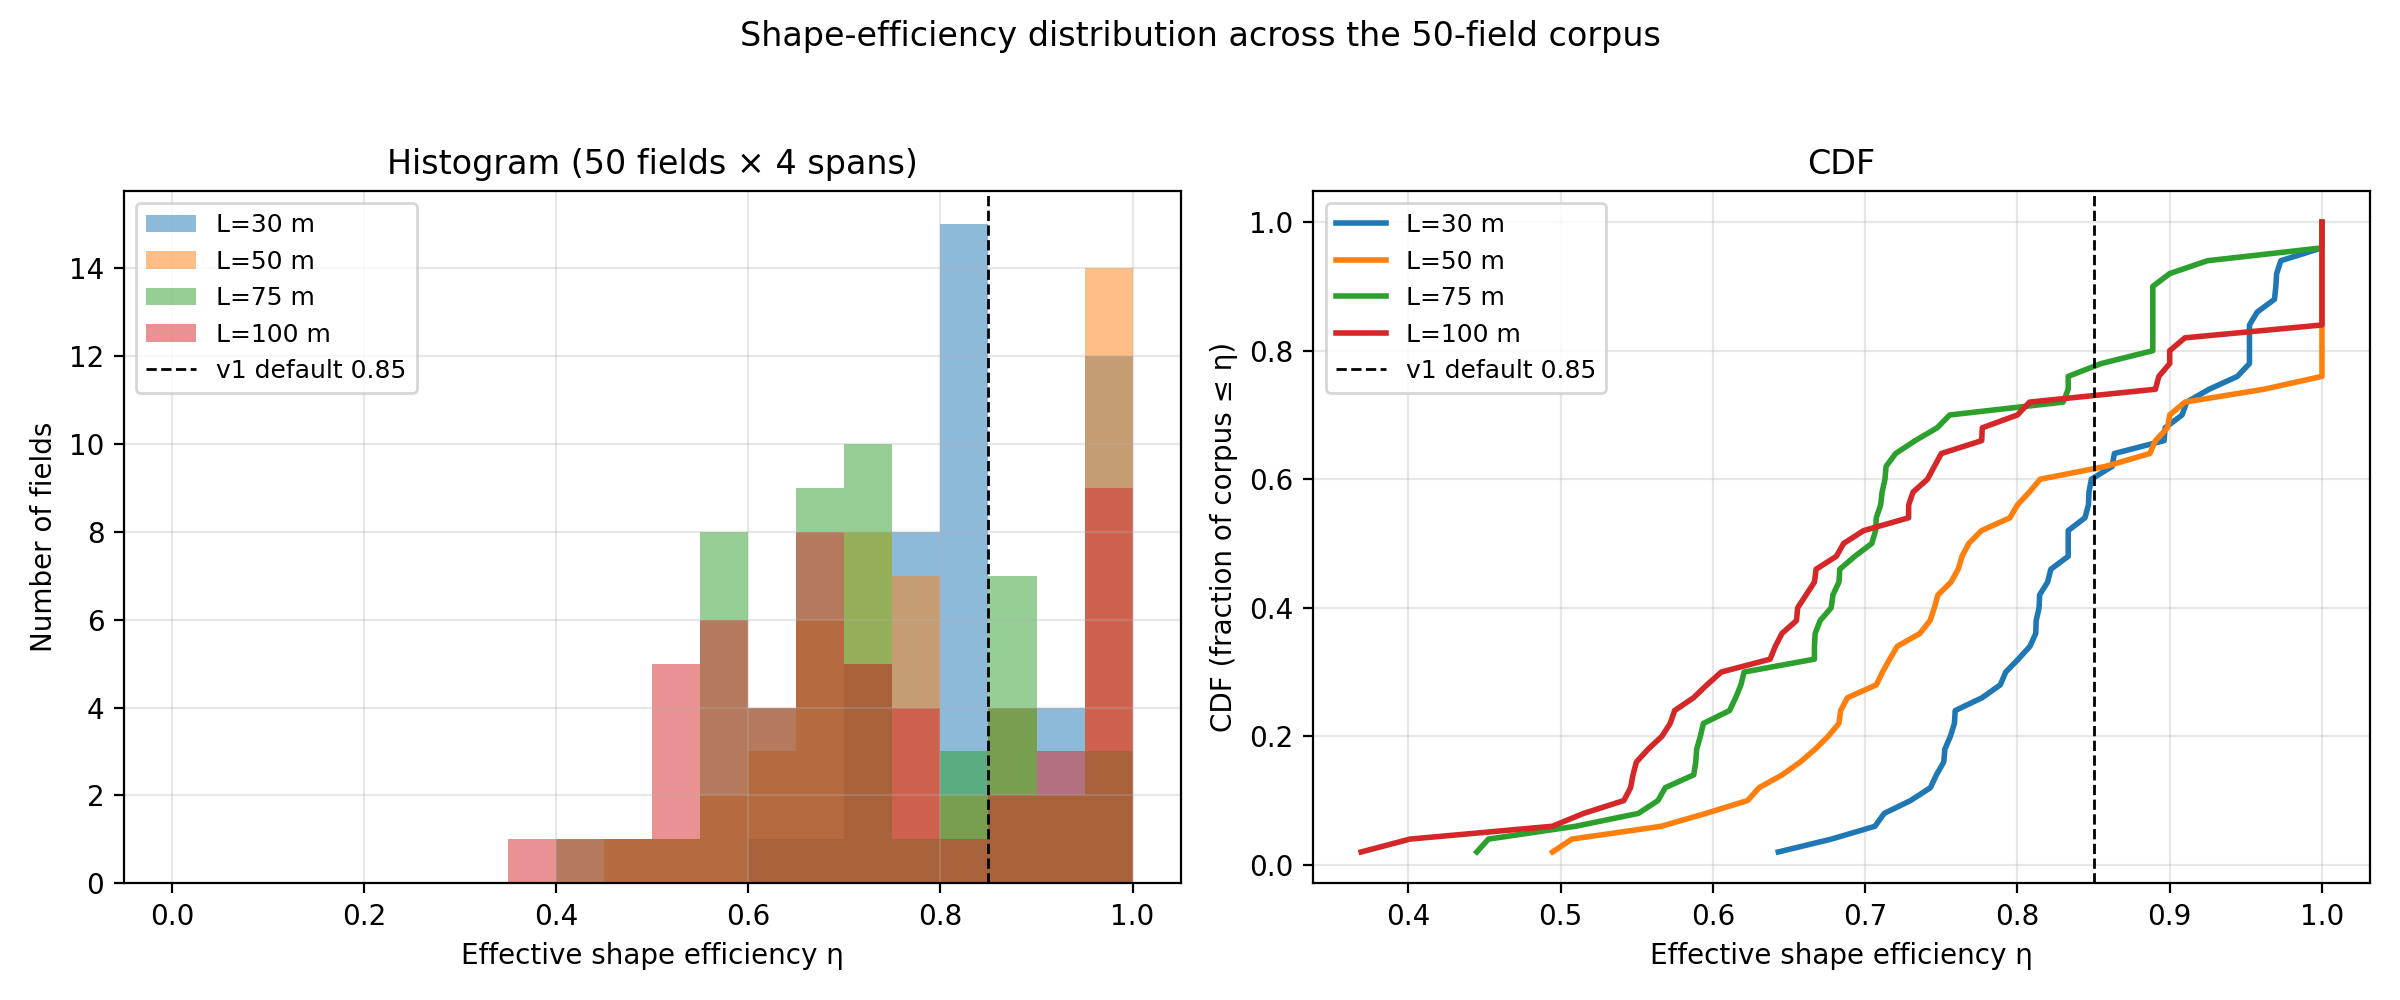
\includegraphics[width=0.85\linewidth]{F9_shape_efficiency_distribution}
\caption{Distribution of best-orientation shape efficiency $\eta$ across the 50-field corpus, by class.}
\label{fig:f9}
\end{figure}

\begin{table}[H]
\centering\small
\caption{Best-orientation shape efficiency $\eta$ by field class at $L = \SI{50}{\meter}$.}\label{tab:eta-classes}
\begin{tabular}{lrrrr}
\toprule
Shape class       & $n$ & Median $\eta$ & P10  & P90 \\
\midrule
rectangle         & 10  & 1.000  & 1.000 & 1.000 \\
L\_shape          & 10  & 0.905  & 0.847 & 1.000 \\
real\_shape       &  5  & 0.800  & 0.776 & 0.862 \\
irregular\_convex & 10  & 0.702  & 0.624 & 0.769 \\
irregular\_concave& 15  & 0.684  & 0.543 & 0.759 \\
\bottomrule
\end{tabular}
\end{table}

\subsubsection{Findings and interpretation}\label{sec:layout-findings}

\textbf{Corpus headline.} The corpus median best-orientation $\eta$ at $L = \SI{50}{\meter}$ is \textbf{0.77}, a 0.08 gap below the 0.85 default that flat feasibility studies typically use. Carrying that gap through the throughput model translates into roughly a 10\,\% throughput reduction on a like-for-like basis. A consistency note that cuts the other way: the paper's own headline numbers (\SI{12.0}{decares\per day}, \SI{1227}{\Wh\per\decare}) are defined on an \emph{ideal} span-commensurate rectangle ($\eta = 1$); on the corpus-median field the same chain delivers ${\approx}0.77\times$ the throughput at ${\approx}1.3\times$ the energy intensity, and readers applying the headline to real parcels should apply that correction. Shape geometry is therefore not a second-order effect that can be folded into a constant; it is a first-order determinant of headline daily area, and it has to be sampled across a corpus rather than picked once.

\textbf{Class structure.} The class breakdown in \cref{tab:eta-classes} explains where the gap comes from and is the more useful number than the corpus median:
\begin{itemize}[leftmargin=1.6em,itemsep=0.15em]
    \item \textbf{Rectangles $\eta = 1.000$ (P10 $=$ P50 $=$ P90).} A disclosure is required here: the corpus rectangles all happen to have their swept side an exact multiple of the \SI{50}{\meter} span, and under \cref{eq:eta-shape} --- which bills the final partial strip block at the full span --- a \emph{non}-commensurate rectangle is not lossless (a $70\times\SI{130}{\meter}$ rectangle scores $\eta \approx 0.87$ at its best orientation). The class median of exactly 1.000 is therefore a corpus-construction artefact; the honest statement is that span-commensurate rectangles are lossless and generic rectangles lose up to one part-span of billed coverage. This quantisation penalty also implies the corpus median below is mildly optimistic.
    \item \textbf{L-shapes $\eta = 0.905$.} A single concave corner costs the planner about 10 percentage points of efficiency, because the strips straddling the missing corner each pay a full Anchor placement to cover a sub-strip-length of polygon. The penalty is bounded and predictable.
    \item \textbf{Real shapes $\eta = 0.800$.} The five hand-traced outlines (river-edge strip, road frontage, pentagon, quarter circle, two-lobe peanut) come in tighter than irregular convex polygons because the irregularity sits along one axis and the planner's orientation sweep can usually find an alignment that suppresses it.
    \item \textbf{Irregular convex $\eta = 0.702$ and irregular concave $\eta = 0.684$.} The two ``hard'' classes converge --- once a polygon is irregular enough that no orientation aligns the strips with a long free edge, adding interior obstacles and concave notches on top of that costs only a further $\sim$2 points. The dominant penalty is failing to find a clean strip axis, not the obstacles themselves.
\end{itemize}
The headline reading is that the architecture is \textbf{geometry-sensitive but not geometry-fragile}: the median field in a deliberately adversarial corpus still recovers 77\,\% of its theoretical throughput. The 12-orientation sweep in \cref{eq:eta-shape} matters here --- a fixed-orientation planner would lose another 5--10 points on the irregular classes, because the optimal sweep direction varies field by field.

\textbf{What CableTract's shape sensitivity tells you about siting.} The class spread implies that shape efficiency is a \emph{site-selection variable}, not a residual error term. A farmer choosing between two candidate parcels of the same area should prefer the rectangular one, and the manuscript carries this through into the operating envelope of \cref{sec:envelope}: the model rewards rectangular plots in solar-rich climates and penalises concave plots in temperate ones.

\textbf{Time budget --- setup is a first-order share, not an overhead.} \Cref{fig:f10} plots three example strip plans. \Cref{fig:f11} plots the time budget to cover a 5-field, \SI{21.2}{\hectare} synthetic farm at the codesigned reference (\SI{1.5}{\meter} swath, \SI{2.2}{\kilo\meter\per\hour} effective operating speed, \SI{60}{\second} anchoring cycle per round): \textbf{operating time ${\approx}\SI{68.3}{\hour}$, setup ${\approx}\SI{52.6}{\hour}$, inter-field travel ${\approx}\SI{0.1}{\hour}$} --- i.e.\ the per-round anchoring cycle consumes \textbf{${\approx}43\,\%$ of the total budget}, in agreement with the ${\approx}27\,\%$ of the daily window the screening model charges (\cref{sec:time}; the farm-scale figure is higher because it also carries per-field alignment). An earlier revision computed this budget at a faster speed, a wider swath, and one setup charge per \SI{50}{\meter} band rather than per round, and concluded the architecture was ``operation-bound'' with a 9\,\% setup share; that conclusion does not survive consistent accounting, and we withdraw it. Two consequences follow:
\begin{itemize}[leftmargin=1.6em,itemsep=0.15em]
    \item Engineering effort on faster or less frequent anchoring is \emph{high-leverage}, not capped: a zero-setup variant would buy back ${\approx}40\,\%$ throughput (and ${\approx}27\,\%$ energy, \cref{sec:anchoring-energy}). This restores the case for the setup-side variants an earlier revision dismissed --- the multi-strip beam anchor (\cref{sec:variant-beam}) and the four-corner CableTract+ (\cref{sec:variant-plus}) are evaluated on exactly this basis.
    \item Faster operation (higher speed within the draft envelope, lower drivetrain losses) still pays roughly $1{:}1$ on the operating slice, so the co-design speed choice remains sound --- but it is no longer the \emph{only} slice worth engineering.
\end{itemize}

\begin{figure}[H]
\centering
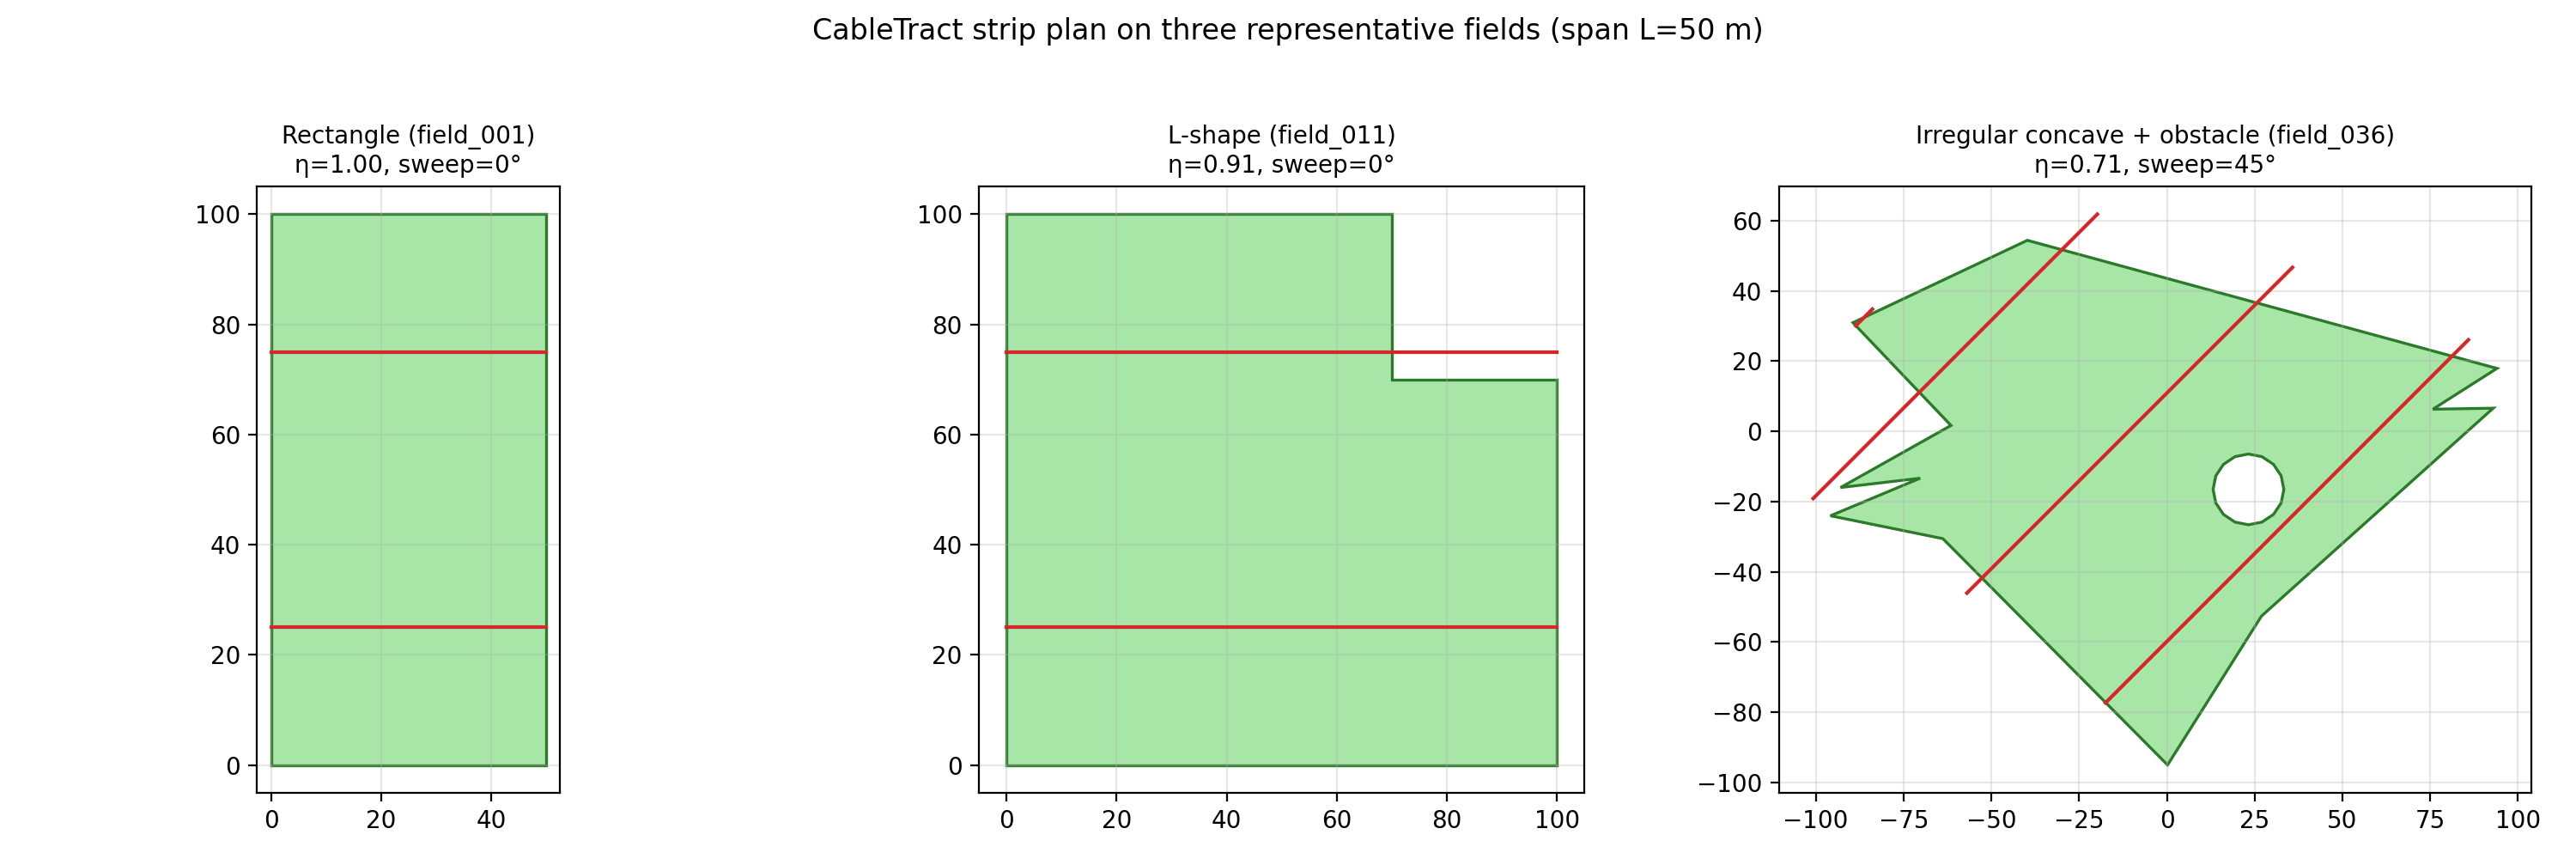
\includegraphics[width=0.95\linewidth]{F10_strip_plans}
\caption{Strip-decomposition plans on three example field shapes (rectangle, L-shape, irregular-concave). Red lines show the per-strip cable lay; green polygons are the field outlines.}
\label{fig:f10}
\end{figure}

\begin{figure}[H]
\centering
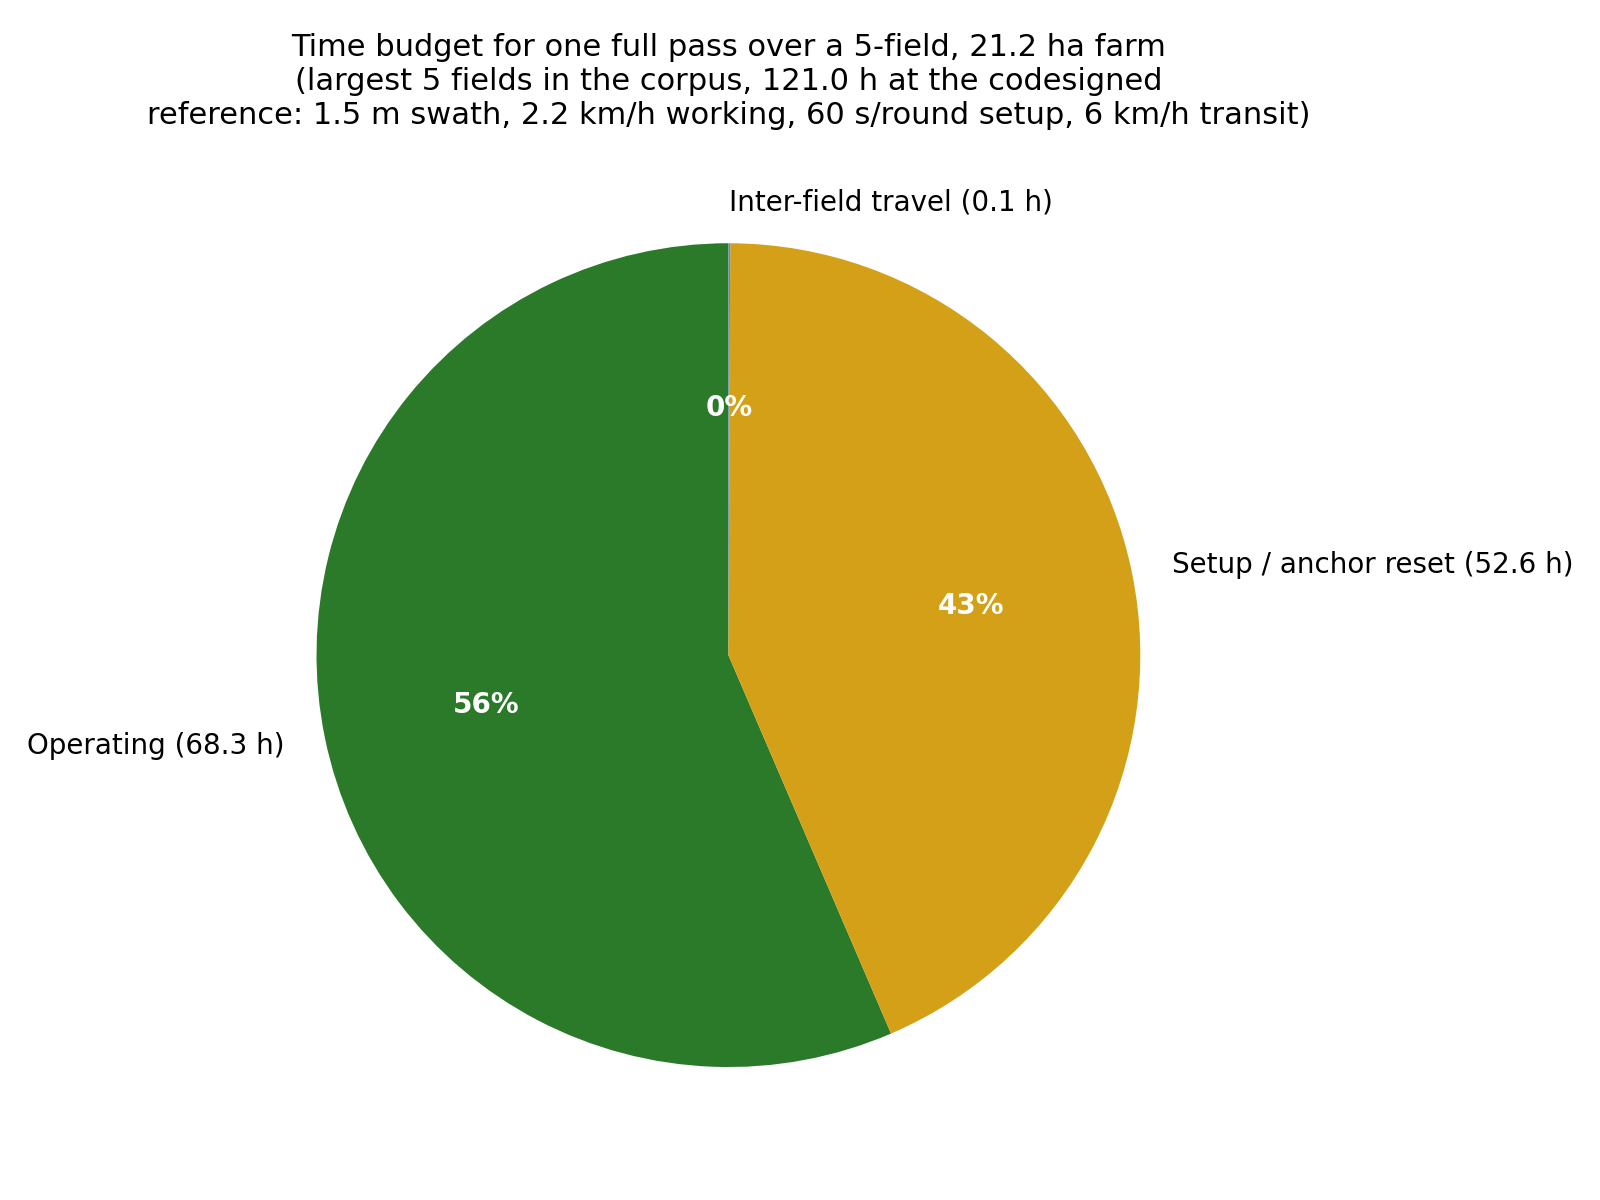
\includegraphics[width=0.65\linewidth]{F11_time_budget}
\caption{Time budget to fully cover a 5-field, \SI{21.2}{\hectare} synthetic farm at the codesigned reference (\SI{1.5}{\meter} swath, \SI{2.2}{\kilo\meter\per\hour} effective speed, \SI{60}{\second} anchoring cycle per round), broken into operation (\SI{68.3}{\hour}), setup (\SI{52.6}{\hour}), and inter-field travel (\SI{0.1}{\hour}). The per-round anchoring cycle is a first-order share (${\approx}43\,\%$) of the budget.}
\label{fig:f11}
\end{figure}

\subsection{Compaction model}\label{sec:compaction}

The compaction story rests on the in-field footprint of CableTract being the \SI{250}{\kilogram} carriage rather than a multi-tonne tractor body. Turning that architectural statement into a defensible per-hectare reduction requires two ingredients: reference contact pressures for an \SI{80}{hp} \gls{wd} tractor drawn from the soil-mechanics literature, and a comparable per-pass compacted-area accounting for the carriage's narrow rollers. \Cref{sec:vehicle-ref,sec:compaction-metrics} provide both.

\subsubsection{Vehicle reference parameters}\label{sec:vehicle-ref}

\begin{table}[H]
\centering\small
\caption{Reference contact pressures for the tractor and the carriage. The reference tractor sits in the \SIrange{100}{250}{\kilo\pascal} band reported by Keller and Lamand\'e (2010)~\cite{keller2010compaction}; the carriage rollers are wide enough to keep per-patch pressure below the ${\sim}\SI{50}{\kilo\pascal}$ subsoil-stress criterion~\cite{schjonning2012rules} at structural weight. Pressures are patch-average values; peak pressures under tyre lugs are typically $2$--$3\times$ the mean~\cite{keller2010compaction}. No stress-propagation/depth modelling is performed --- the $p^2$ index below is a S\"ohne-inspired severity proxy, not a bulk-density prediction.}\label{tab:vehicle-pressures}
\begin{tabular}{lcrrr}
\toprule
Vehicle & Wheels & Total mass & Mean $p$ (kPa) & Max $p$ (kPa) \\
\midrule
Reference \SI{80}{hp} \gls{wd} tractor & 4 (front+rear) & ${\approx}\SI{4}{\tonne}$  & \textbf{143} & \textbf{150} \\
CableTract carriage                    & 2 wide rollers & ${\approx}\SI{250}{\kilogram}$ & \textbf{31}  & \textbf{31}  \\
\bottomrule
\end{tabular}
\end{table}

\subsubsection{Compacted-area and contact-energy metrics}\label{sec:compaction-metrics}

For each (vehicle, field) pair we compute five scalar compaction metrics:

\begin{itemize}[leftmargin=1.6em,itemsep=0.1em]
    \item \textbf{Trafficked area (\si{\meter\squared}).} For the tractor: polygon area $\times$ per-pass tyre-track coverage ($2\times\SI{0.45}{\meter}$ of track over a \SI{1.8}{\meter} gauge $= 50\,\%$) $\times$ pass count. For the carriage: \emph{one roller traverse per swath} --- covered area $\times$ (total track width / swath width) $\times$ pass count $= 0.4/1.5 \approx 26.7\,\%$ per pass. (An earlier revision billed the carriage one traverse per \SI{50}{\meter} span band --- one thirty-third of its true rolling distance --- which produced a spurious ${\sim}98\,\%$ area-reduction headline; the correction below is the single largest numerical change of this revision.)
    \item \textbf{Trafficked area fraction.} Trafficked area / (polygon area $\times$ pass count).
    \item \textbf{Mean pressure (\si{\kilo\pascal}).} Load-weighted mean of all wheel contact pressures.
    \item \textbf{Per-running-gear contact-energy index.} $\sum p^{2} \cdot A_{\text{patch}} \cdot \text{pass\_count}$ over the instantaneous contact patches (\si{\kilo\pascal\squared.\meter\squared}) --- a property of the running gear. The $p^2$ weighting is motivated by elastic strain-energy density scaling as $\sigma^2$ (stress itself propagates linearly with surface load in the Boussinesq/S\"ohne framework~\cite{sohne1953druck}).
    \item \textbf{Field-integrated $p^2$ exposure.} Mean pressure squared $\times$ trafficked area $\times$ passes --- the honest field-level combination of the pressure and area effects.
\end{itemize}

A 4-pass cropping season is the default.

\subsubsection{Compaction map}\label{sec:f12}

\begin{figure}[H]
\centering
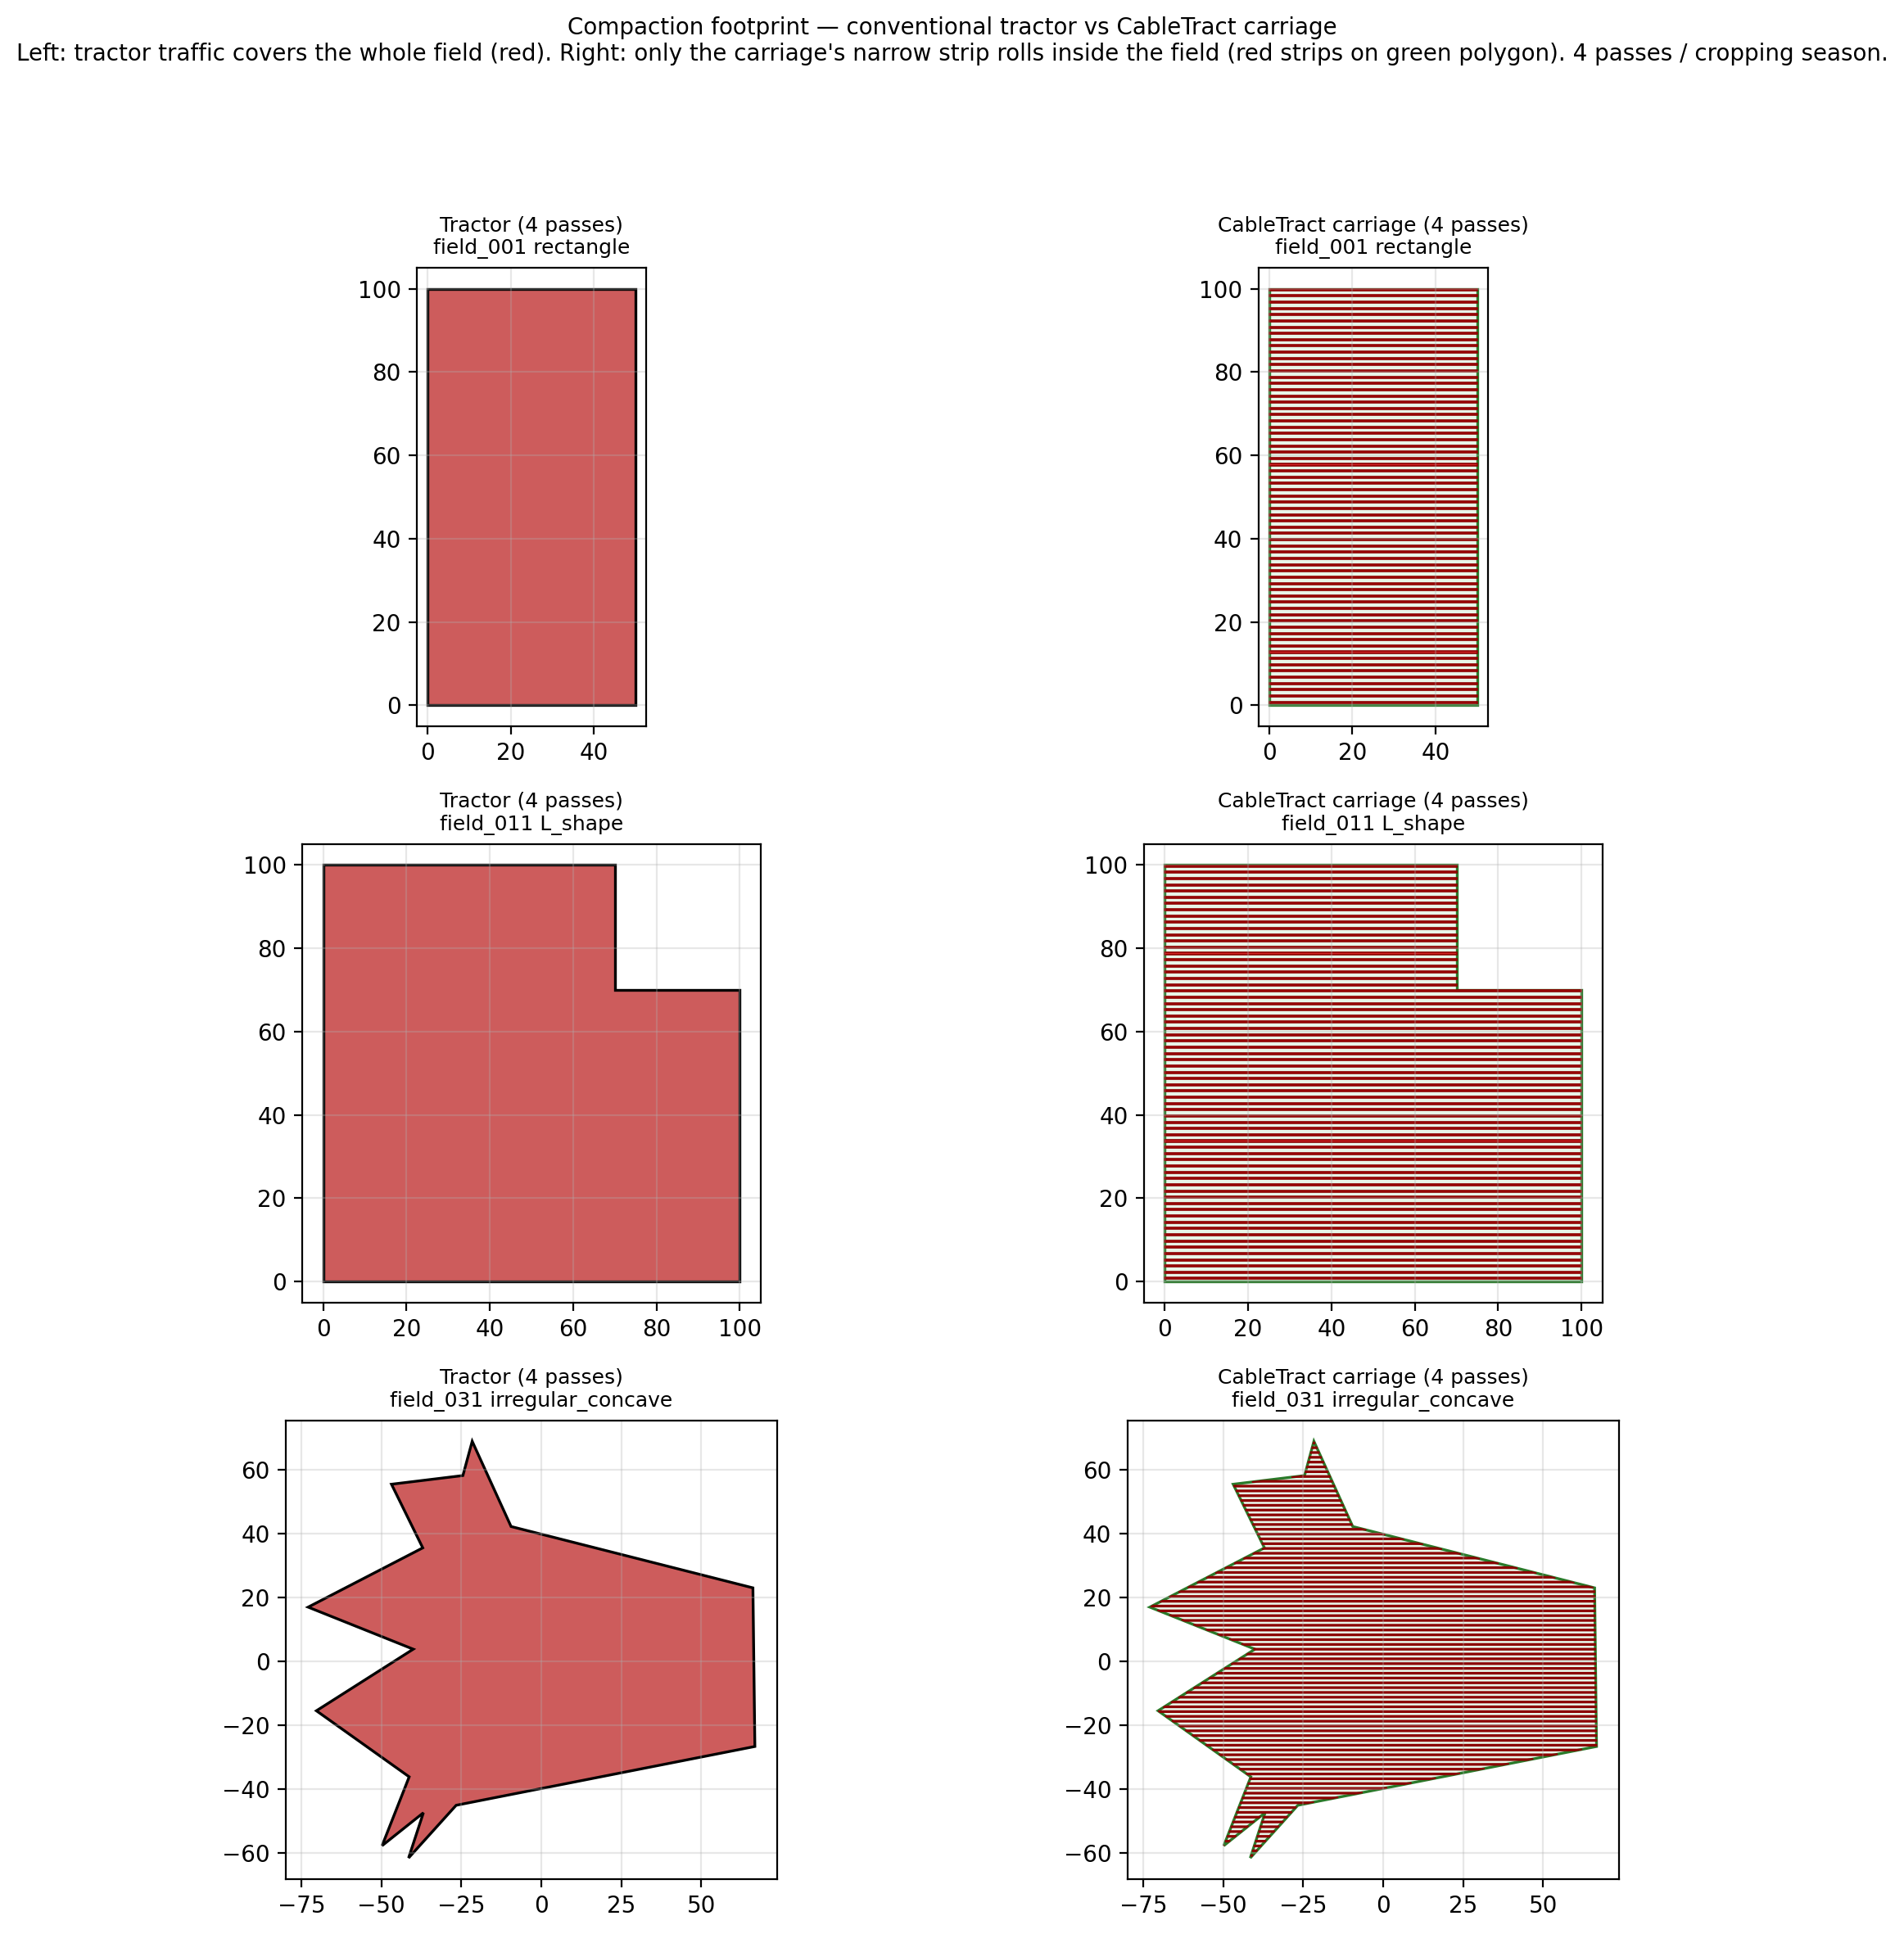
\includegraphics[width=0.95\linewidth]{F12_compaction_map}
\caption{Compaction comparison on three field classes (rectangle, L-shape, irregular-concave). Left panels: the tractor's seasonal footprint (filled: its tyre tracks cover 50\,\% of the field on each of 4 passes). Right panels: the carriage's roller tracks (red bands, one \SI{0.4}{\meter} track per \SI{1.5}{\meter} swath) on the field polygon (green).}
\label{fig:f12}
\end{figure}

\begin{table}[H]
\centering\small
\caption{Per-field compaction summary with the corrected per-swath carriage accounting. The per-running-gear index reduction ($73\times$) combines the $4.6\times$ lower mean pressure (squared, ${\approx}21\times$) with the ${\approx}3.5\times$ smaller contact area and is field-independent; the field-integrated $p^2$ exposure additionally weights by trafficked area.}\label{tab:compaction}
\resizebox{\textwidth}{!}{%
\begin{tabular}{lllrrrrr}
\toprule
Field & Class & & Tractor trafficked & Carriage trafficked & Area reduction & Gear index & Field-integrated $p^2$ \\
\midrule
field\_001 & rectangle         & & 50\,\% & 26.7\,\% & 47\,\% & $73\times$ & $39\times$ \\
field\_011 & L\_shape          & & 50\,\% & 26.7\,\% & 47\,\% & $73\times$ & $39\times$ \\
field\_031 & irregular\_concave& & 50\,\% & 26.7\,\% & 47\,\% & $73\times$ & $39\times$ \\
\bottomrule
\end{tabular}%
}
\end{table}

\textbf{CableTract roughly halves the trafficked area} (${\approx}27\,\%$ vs ${\approx}50\,\%$ of field area per pass) --- a useful but not extraordinary reduction, comparable to what \gls{ctf} achieves with conventional machinery (\cref{sec:related-ctf}). \textbf{The architecture's distinctive compaction gain is in pressure, not area}: the carriage's \SI{31}{\kilo\pascal} mean contact pressure is $4.6\times$ below the tractor's \SI{143}{\kilo\pascal} and below the ${\sim}\SI{50}{\kilo\pascal}$ subsoil-stress criterion~\cite{schjonning2012rules}, so the \emph{field-integrated $p^2$-weighted exposure drops ${\approx}39\times$} and the per-running-gear index ${\approx}73\times$.

Three caveats keep this honest. First, the carriage roller load here is its structural weight only; during tillage the S1 down-pressure reserve (\cref{sec:v-s1}, ${\approx}\SI{1.75}{\kilo\newton}$) and tool reactions raise the total vertical load to ${\approx}\SI{4.2}{\kilo\newton}$, i.e.\ ${\approx}\SI{52}{\kilo\pascal}$ mean pressure --- at the criterion rather than comfortably below it --- and the field-integrated advantage during tillage passes drops to ${\approx}14\times$ (still above the C1 threshold of $20\times$ when averaged over the 4-pass season, of which at most one is a heavy-downforce pass; a loaded sprayer or seed hopper has a similar effect). Second, the heavy modules' own lanes --- one \gls{mu}/Anchor lane per \SI{50}{\meter} band plus the Anchor's deployment crossing --- traffic a further ${\approx}\SIrange{2}{4}{\percent}$ of the field at near-tractor pressures on deeper fields; counted against CableTract, this trims the area reduction by a few points and the field-integrated advantage to ${\approx}\SIrange{30}{35}{\times}$. Third, richer dynamic models would move \emph{both} sides: multi-pass deformation and dynamic load transfer add compaction to the tractor, while repeated trafficking of the carriage's tracks and the lower effective pressure of deflected radial tyres (\SIrange{80}{120}{\kilo\pascal}) push the other way. We report the static comparison and do not claim that the dynamic case can only favour CableTract.

\subsection{Uncertainty quantification and global sensitivity}\label{sec:uq}

Every number in \cref{sec:physics,sec:soil,sec:energy,sec:economics,sec:layout,sec:compaction} depends on parameters whose values are known to within published uncertainty bands rather than exactly. A defensible feasibility envelope must therefore answer two questions: given the joint uncertainty in 20 parameters, what is the \textbf{P10--P90 envelope} of the headline outputs, and which parameters carry the most variance --- in particular, is any single parameter still dominant after the \cref{sec:drivetrain} decomposition of the lumped drivetrain efficiency? We answer the first with a 1\,000-sample Monte Carlo and the second with a Sobol global sensitivity decomposition~\cite{sobol2001indices,saltelli2008primer} computed via \gls{salib}~\cite{herman2017salib,iwanaga2022salib}.

\subsubsection{Parameter problem}\label{sec:uq-problem}

The uncertainty problem is defined over 20 parameters drawn from physically defensible bands with uniform marginals. Examples:

\begin{itemize}[leftmargin=1.6em,itemsep=0.1em]
    \item Lumped drivetrain efficiency $\in [0.35, 0.65]$ --- covers the manufacturer datasheet range for industrial \gls{pmsm}/gearbox/drum/cable chains after the \cref{sec:drivetrain} decomposition.
    \item Draft load $\in [\SI{1500}{\newton}, \SI{4500}{\newton}]$ --- spans the codesigned-library P10--P90 envelope from \cref{sec:soil}.
    \item Shape efficiency $\in [0.55, 1.00]$ --- covers the entire field-corpus range from \cref{fig:f9}.
    \item PV area $\in [\SI{10}{\meter\squared}, \SI{30}{\meter\squared}]$ and battery capacity $\in [\SI{5}{\kWh}, \SI{25}{\kWh}]$ --- spans the design envelope of \cref{fig:f8}.
\end{itemize}

These bands are deliberately wider than typical sensitivity studies on energy systems, so the resulting Sobol decomposition is hard to fudge.

\subsubsection{Monte Carlo}\label{sec:mc}

We draw $n = 1000$ samples from the joint distribution and evaluate the full simulator on each. Doubling the sample size to 2000 shifts \gls{p50} by ${\approx}2\,\%$ and \gls{p10}/\gls{p90} by up to ${\approx}4\,\%$ for the throughput target (well under 1\,\% for energy per decare), adequate for a screening envelope. \Cref{fig:f15} plots the resulting throughput envelope versus draft load, with the codesigned reference (\SI{1800}{\newton}, \SI{12.0}{decares\per day}) overlaid as a green star. The star sits below the \gls{p50} line at the same draft but well inside the P10--P90 envelope, which is the expected behaviour: the reference sits at the extreme low edge of the sampled width band (\SI{1.5}{\meter} in $[1.5, 3.0]$) and below the PV-area and battery-band midpoints, so it should land in the lower half of the joint distribution rather than at its centre. The Monte Carlo run is a check on robustness, not a re-derivation of the codesigned point.

\begin{figure}[H]
\centering

\includegraphics[width=0.85\linewidth]{F15_mc_throughput_envelope}
\caption{Monte Carlo throughput envelope versus draft load (1\,000 samples). Codesigned reference overlaid as a green star.}
\label{fig:f15}
\end{figure}

\subsubsection{Global sensitivity}\label{sec:sobol}

First-order (\gls{sobol1}) and total-order (\gls{sobolt}) Sobol indices~\cite{sobol2001indices} are estimated with the Saltelli sampler~\cite{saltelli2008primer,herman2017salib} at $n_{\text{base}} = 256$ without second-order terms, giving $256 \times (20 + 2) = 5\,632$ simulator evaluations per Sobol pass. The four targets are daily off-grid throughput, energy per decare, payback versus diesel, and surplus power. Two scope notes: battery capacity is sampled but has zero index by construction (in the screening chain pack size gates only a feasibility flag, not the outputs --- a real system's throughput would depend on it, which the hourly model of \cref{sec:energy} captures instead); and no anchor-capacity or soil-strength parameter is sampled, so the Sobol result says nothing about geotechnical risk --- the anchor envelope of \cref{sec:anchor} acts as a hard gate outside the UQ.

\begin{figure}[H]
\centering

\includegraphics[width=0.95\linewidth]{F13_sobol_bars}
\caption{Sobol \gls{sobol1} and \gls{sobolt} indices for the top-12 parameters across the four headline outputs. After the \cref{sec:drivetrain} decomposition of the lumped drivetrain efficiency, no single parameter exceeds ${\approx}0.25$ total-order on throughput.}
\label{fig:f13}
\end{figure}

\textbf{The throughput variance is diffuse.} For daily throughput, the largest contributors --- PV area ($\gls{sobolt} = 0.245$), daily solar hours (0.226), draft load (0.189), strip width (0.142), and irradiance intensity (0.135) --- each sit in the band $\gls{sobolt} \approx 0.13$--$0.25$; their \emph{first-order} indices sum to ${\approx}0.65$ of the variance (total-order indices overlap through interactions and cannot be summed as shares). No single parameter exceeds ${\approx}0.25$ total-order on throughput; the diffuseness claim is specific to the throughput target (setup time, for instance, dominates the surplus-power target). The codesigned reference is not a hand-tuned local optimum sitting on top of one undefended fudge factor; it is robust to the full joint uncertainty in the 20 inputs.

\subsubsection{Tornado on NPV}\label{sec:tornado}

\textbf{What this analysis answers.} The Sobol decomposition in \cref{fig:f13} asks where throughput \emph{variance} comes from. The sceptical financial reviewer asks something more direct: \emph{which single economic inputs, varied across realistic bounds, move the NPV most --- and can any of them flip the sign?} \Cref{fig:f14} answers this by perturbing each economic driver one at a time around the codesigned reference (\cref{tab:econparams}) while holding the rest fixed, and sorting by the resulting NPV swing.

\textbf{The frame.} To keep the tornado consistent with the rest of the economics, its baseline is the same \emph{replacement-frame} NPV reported in \cref{tab:npv-farmsize}: \SI{-1724}{\EUR} at \SI{25}{\hectare\per\year}, 8\,\%, 15-year horizon, against a like-for-like used diesel tractor (machine capex increment \SI{3670}{\EUR}). The annual area is held at the \SI{25}{\hectare\per\year} reference and diesel at \SI{12}{\litre\per\hectare} throughout, so each swing is read against the same operating point used elsewhere in the paper rather than against the machine's full throughput capacity.

\begin{figure}[H]
\centering

\includegraphics[width=0.85\linewidth]{F14_tornado_npv}
\caption{Tornado plot of one-at-a-time NPV-vs-diesel sensitivities to the economic drivers, at the codesigned reference in the replacement frame (\SI{25}{\hectare\per\year}, 8\,\% discount, 15-yr horizon, machine capex increment \SI{3670}{\EUR}). Baseline NPV \SI{-1724}{\EUR} (dashed); the dotted line marks NPV\,$=0$ (break-even vs diesel). Each bar moves one parameter to its favourable/adverse bound while all others stay at the reference. Sorted top to bottom by total swing.}
\label{fig:f14}
\end{figure}

\textbf{What the tornado shows.} At the \SI{25}{\hectare\per\year} reference the NPV sits close to zero (\SI{-1724}{\EUR}), so \emph{most} single drivers can flip its sign --- eight of the twelve do at their bounds. The largest swings are:
\begin{itemize}[leftmargin=1.6em,itemsep=0.15em]
    \item \textbf{The used diesel-tractor price.} A cheaper used tractor (\SI{30}{\kilo\EUR}) drops the NPV to ${\approx}\SI{-8.9}{\kilo\EUR}$; a dearer one (\SI{45}{\kilo\EUR}) lifts it to ${\approx}\SI{+12.6}{\kilo\EUR}$ --- a \SI{21.4}{\kilo\EUR} swing, the single most influential parameter.
    \item \textbf{The maintenance basis.} The CableTract maintenance fraction ($0.02\to0.06$ of machine capex) swings the NPV by \SI{13.2}{\kilo\EUR}, and the diesel fraction ($0.03\to0.07$) by \SI{12.0}{\kilo\EUR}. Both are flat calendar-based assumptions; under an hour-based (EP496-style) basis, a tractor used only ${\sim}\SIrange{35}{50}{\hour\per\year}$ at \SI{25}{\hectare\per\year} would incur only a few hundred euro of R\&M per year, which moves the reference NPV further negative --- the flat basis is defensible for an aged machine's calendar-dominated costs (insurance, housing, perishing components) but the reader should know the result leans on it.
    \item \textbf{Farm size.} 10$\to$\SI{100}{\hectare\per\year} moves NPV from ${\approx}\SI{-3.9}{\kilo\EUR}$ to ${\approx}\SI{+9.1}{\kilo\EUR}$ --- the dominant upside lever and the axis along which the sign robustly turns.
    \item \textbf{Main-Unit and Anchor capex, battery size and price, diesel price and volume} each contribute swings of \SIrange{2.5}{10.7}{\kilo\EUR}.
\end{itemize}

\textbf{Honest reading.} A reference point this close to break-even cannot support a categorical claim in either direction, and we do not make one. What the tornado \emph{does} establish: (i) the largest single swing is exogenous (the price of the diesel alternative), so the result is as much a statement about used-tractor markets as about CableTract; (ii) farm size is the one axis along which the sign turns robustly positive (\cref{sec:npv-farmsize}); and (iii) the labour line excluded from both sides (a tractor needs a driver for every hour; CableTract needs supervision whose legal minimum is unresolved, \cref{sec:open-risks}) is plausibly larger than every bar in the figure --- autonomy, if certified, is the biggest unmodelled upside, and mandatory on-site supervision would cancel it. The economic case is therefore best stated as ``cost-parity at \SI{25}{\hectare\per\year} within parameter uncertainty, robustly positive above ${\sim}\SI{40}{\hectare\per\year}$'', not as favourable-everywhere. The additive-purchase frame is far weaker still (\cref{tab:cashflow}) and we report it explicitly.

\subsubsection{NPV vs farm size}\label{sec:npv-farmsize}

\Cref{fig:f16} sweeps the discounted-cash-flow chain over six farm sizes (1, 5, 10, 25, 50, 100 ha/yr) at three discount rates (5/8/12\,\%). At the codesigned reference (\cref{tab:npv-farmsize}):

\begin{table}[H]
\centering\small
\caption{NPV vs diesel and discounted payback at six farm sizes and three discount rates (replacement frame; carriage costed, implement sets netted, cable line included). Bold row is the codesigned reference (\SI{25}{\hectare\per\year}, 8\,\%). Payback is capped at the 15-yr horizon.}\label{tab:npv-farmsize}
\resizebox{\textwidth}{!}{%
\begin{tabular}{rrrrr}
\toprule
Farm size (\si{\hectare\per\year}) & NPV @ 5\,\% (\si{\EUR}) & NPV @ 8\,\% (\si{\EUR}) & NPV @ 12\,\% (\si{\EUR}) & Payback @ 8\,\% (\si{\year}) \\
\midrule
1   & $-5\,570$  & $-5\,175$  & $-4\,779$  & $>15$ \\
5   & $-4\,872$  & $-4\,600$  & $-4\,321$  & $>15$ \\
10  & $-4\,000$  & $-3\,881$  & $-3\,749$  & $>15$ \\
\textbf{25}  & $\mathbf{-1\,385}$  & $\mathbf{-1\,724}$  & $\mathbf{-2\,033}$  & \textbf{${\approx}14$} \\
50  & $+2\,975$  & $+1\,871$  & $+828$     & 5.4 \\
100 & $+11\,694$ & $+9\,061$  & $+6\,549$  & 2.5 \\
\bottomrule
\end{tabular}%
}
\end{table}

\begin{figure}[H]
\centering

\includegraphics[width=0.85\linewidth]{F16_npv_vs_farm_size}
\caption{\gls{npv} vs diesel as a function of farm size at three discount rates (panel a), the corresponding discounted payback (panel b), and the levelised cost of operation (panel c). The replacement-frame NPV crosses zero near \SI{40}{\hectare\per\year} at all three discount rates.}
\label{fig:f16}
\end{figure}

\textbf{In the replacement frame, the economics are scale-conditional: NPV is negative below ${\sim}\SI{40}{\hectare\per\year}$ and positive above, at all three discount rates.} This is the central economic finding. At the \SI{25}{\hectare\per\year} reference the machine is approximately cost-neutral (\SI{-1.7}{\kilo\EUR} over 15 years, within the uncertainty of nearly every input, \cref{sec:tornado}); at \SI{50}{\hectare\per\year} the NPV is \SI{+1.9}{\kilo\EUR} with a 5.4-year payback, and at \SI{100}{\hectare\per\year} it is \SI{+9.1}{\kilo\EUR} with a 2.5-year payback. The intuition: the \SI{3670}{\EUR} machine increment and the ${\approx}\SI{620}{\EUR\per\year}$ of fixed opex differential are covered by fuel savings that scale with area (\SI{16.8}{\EUR\per\hectare}), so the case strengthens roughly linearly with annual area and diesel price. An \emph{additive} buyer who finances the full \SI{48170}{\EUR} system without retiring a tractor sees \SI{-61}{\kilo\EUR} at \SI{25}{\hectare\per\year}, and no single machine reaches the additive break-even within its own capacity (\cref{tab:cashflow}).

\begin{figure}[H]
\centering

\includegraphics[width=0.85\linewidth]{F17_lca_co2}
\caption{Lifecycle CO\textsubscript{2} per hectare-year for CableTract, the diesel reference tractor, and a Monarch-class electric tractor (stacked: embodied + fuel/grid). CableTract delivers a $1.9\times$ improvement over diesel that does not depend on grid decarbonisation.}
\label{fig:f17}
\end{figure}

\subsection{Architectural variants}\label{sec:ml}

\subsubsection{What this section is for}\label{sec:variants-intro}

Everything up to this point has analysed a single architecture: the codesigned two-module design --- one stationary Main Unit, one Anchor, a single tensioned cable, and a four-quadrant drivetrain with regenerative braking on the unloaded return leg (the default, \cref{sec:drivetrain}). The natural next question is whether that design is the only sensible point in the design space, or whether topological modifications --- adding more Main Units, or conversely dropping the regen drive --- materially change the headline numbers. We answer this with a small, deliberately narrow comparison: \textbf{four configurations run on the same codesigned parameter set, on the same simulator, so the resulting bars are directly comparable}.

Each is implemented as a \emph{parameter transformation} on the codesigned reference of \cref{tab:codesigned-params}, fed into the same \texttt{run\_single} routine, with no parallel code path. The result is a clean apples-to-apples comparison rather than three independent feasibility studies that drift apart on definitions.

\begin{itemize}[leftmargin=1.6em,itemsep=0.15em]
    \item \textbf{Codesigned baseline (regen default)} (\cref{sec:variant-baseline}): the default architecture as analysed in \cref{sec:physics,sec:soil,sec:energy,sec:economics}. One Main Unit, one Anchor, one cable, and four-quadrant regenerative braking on the return leg. This is the reference column of \cref{tab:variants-numbers}.
    \item \textbf{Multi-strip anchoring --- beam and travelling sheave} (\cref{sec:variant-beam}): both modules anchor once per block of $k$ strips; between strips only a sheave trolley indexes laterally along a rigid transverse beam. Attacks the same per-round anchoring cycle at a fraction of CableTract+'s capital.
    \item \textbf{CableTract+, the four-Main-Unit planar cable robot} (\cref{sec:variant-plus}): four corner stations and two simultaneously-pulling cables, so the carriage moves in a 2-D plane between the corners instead of along a 1-D strip. Eliminates the anchoring cycle entirely (the 27\,\% energy and ${\approx}30$--$43\,\%$ time share of \cref{sec:anchoring-energy,sec:layout-findings}) at the price of four Main Units.
    \item \textbf{Unidirectional drivetrain (no regen)} (\cref{sec:variant-norering}): the same two-module architecture with a plain one-way drivetrain in place of the four-quadrant regen drive --- \SI{300}{\EUR} cheaper, but forgoing the return-leg recovery. Quantifies what the regen default buys.
\end{itemize}

An earlier revision dismissed all setup-side variants on the ground that setup was ``only 9\,\% of the time budget''; the corrected accounting (setup ${\approx}\SIrange{27}{43}{\percent}$ of time and 27\,\% of energy) reverses that judgement, and the multi-strip anchoring concept is therefore now evaluated quantitatively as a full variant (\cref{sec:variant-beam}). A note on geometry: the \emph{naive} realisation --- a sheave that merely swivels about a vertical pivot on a point-anchored module --- does \emph{not} work, because passes then fan out from the fixed end and overlap near the pivot, wasting roughly half of each pass in re-tilled ground; the beam-and-trolley mechanism of \cref{sec:variant-beam} is what preserves parallel strips. A drone-assisted inter-field alignment variant remains deferred (\cref{sec:variants-named}).

\begin{table}[H]
\centering\small
\caption{Architectural variant comparison on the codesigned reference parameter set. All four rows are run on the same \texttt{run\_single} call, with the variant differences applied as parameter transformations on top of \cref{tab:codesigned-params}. CAPEX is the itemised \cref{sec:economics} machine bill of materials in 2024 EUR. ``Simple payback'' is the undiscounted ratio of the sales price (CAPEX $\times 1.33$ sales margin) to annual diesel-fuel savings \emph{at the machine's full energy-limited utilisation} (${\approx}\SI{204}{\hectare\per\year}$ for the baseline) --- an additive-buyer stress frame, deliberately different from the \cref{sec:economics} replacement chain at \SI{25}{\hectare\per\year}; see \cref{sec:variants-discussion} for the reconciliation.}\label{tab:variants-numbers}
\resizebox{\textwidth}{!}{%
\begin{tabular}{lrrrrr}
\toprule
Variant & Throughput (dec/day) & Energy/decare (Wh) & CAPEX (\si{\EUR}) & Simple payback (mo) & Surplus (W) \\
\midrule
\textbf{Codesigned baseline (regen)} & \textbf{12.0} & \textbf{1\,227} & \textbf{38\,670} & \textbf{180.3} & \textbf{1\,036} \\
Multi-strip anchoring (beam, $k=4$) & 14.5 ($\boldsymbol{1.21\times}$) & 974 ($\boldsymbol{0.79\times}$) & 40\,170 ($1.04\times$) & 148.7 ($\boldsymbol{0.82\times}$) & 891 \\
CableTract+ (4-MU robot)         & 16.5 ($1.37\times$) & 889 ($0.73\times$) & 84\,997 ($2.20\times$) & 287.4 ($1.59\times$) & 970 \\
Unidirectional (no regen)        & 11.7 ($0.97\times$) & 1\,259 ($1.03\times$) & 38\,370 ($0.99\times$) & 183.6 ($1.02\times$) & 1\,036 \\
\bottomrule
\end{tabular}%
}
\end{table}

\begin{figure}[H]
\centering

\includegraphics[width=0.95\linewidth]{F20_variant_comparison}
\caption{Architectural variant comparison on the codesigned reference parameter set. Codesigned baseline outlined in black. Lower is better for energy, CAPEX, and payback; higher is better for throughput and surplus power.}
\label{fig:f20}
\end{figure}

\subsubsection{Variant 1 --- Codesigned baseline (regen default)}\label{sec:variant-baseline}

This is the default architecture analysed throughout the paper: one Main Unit (PMSM + winch + drum + battery + PV/wind energy harvester) at one end of the strip, one Anchor (ground-screw module that resists the cable reaction) at the other, one Dyneema cable loop spanning between them at typical span $L = \SI{50}{\meter}$, and a soil-supported implement carriage towed along the strip. The drivetrain is \emph{four-quadrant}: the motor pulls the carriage outbound under load, and on downhill return legs it recovers a modest amount of energy back into the battery (\cref{sec:drivetrain}; ${\approx}0$ on flat ground). Setup between strips is the full anchoring cycle of \cref{sec:anchoring-energy}. The baseline column of \cref{tab:variants-numbers} is the deterministic \texttt{run\_single} output at the codesigned parameter set: \textbf{12.0 decares/day off-grid throughput, 1\,227 Wh/decare energy intensity (anchoring charged), \SI{38670}{\EUR} machine CAPEX, 180.3-month simple payback in the table's additive stress frame, and ${\approx}\SI{1040}{\watt}$ of surplus power} (harvested PV/wind minus operating draw and idle housekeeping). This is the reference against which the next two rows are read.

\subsubsection{Variant 2 --- Multi-strip anchoring (beam + travelling sheave)}\label{sec:variant-beam}

The second configuration attacks the anchoring cycle directly, with minimal new hardware. The Anchor gains a rigid \textbf{transverse beam} (${\approx}\SI{4.5}{\meter}$, folded for transport) planted \emph{once} per block of $k$ strips by the 9-screw cluster; the redirect sheave rides this beam on a \textbf{travelling trolley}. The \gls{mu} likewise anchors once per block --- between strips it holds the cable reaction by braked wheels alone, which its own weight makes credible on firm ground (${\approx}\SI{13.7}{\kilo\newton}$ on the wheels at $\mu \approx 0.4$--$0.5$ gives \SIrange{5.5}{7}{\kilo\newton} of holding friction against the \SI{3.0}{\kilo\newton} P90 pull; its four screws remain available for soft or sloped headlands). The operating cycle then splits into two tiers:

\begin{itemize}[leftmargin=1.6em,itemsep=0.1em]
    \item \textbf{Per strip} ($k-1$ of every $k$ rounds): tool retracts, both take-off points index \SI{1.5}{\meter} laterally (trolley on the Anchor beam; the \gls{mu} rolls on braked wheels), re-tension --- ${\approx}\SI{15}{\second}$ and essentially zero anchoring energy.
    \item \textbf{Per block} (once every $k$ strips): the full 13-screw anchoring cycle of \cref{sec:anchoring-energy} plus a $k \times \SI{1.5}{\meter}$ roll --- ${\approx}\SI{75}{\second}$ and \SI{25.3}{\Wh}.
\end{itemize}

The strips stay exactly parallel because the take-off \emph{point} translates while the anchored \emph{structure} does not --- which is what the naive swivelling-sheave realisation gets wrong (\cref{sec:variants-intro}). At $k=4$ the mean setup time falls from \SI{60}{} to \SI{30}{\second\per round} and the anchoring energy from \SI{25.3}{} to \SI{6.3}{\Wh\per round}, giving \textbf{14.5 decares/day ($1.21\times$), \SI{974}{\Wh\per\decare} ($0.79\times$), and the best simple payback in the table ($0.82\times$ baseline)} for a ${\approx}\SI{1500}{\EUR}$ beam-and-trolley increment.

\textbf{What limits $k$ is the anchor load path, not the mechanism.} With the trolley at the beam end, the cable pull acts at an offset of $(k-1)/2 \times \SI{1.5}{\meter}$ from the cluster centre, and the resulting yaw moment is resisted as differential lateral loads on the cluster's outer screw rows ($M / (\SI{1.2}{\meter} \times 3)$ per screw for the $3\times3$ cluster). At the codesigned P90 of \SI{3.0}{\kilo\newton}: $k=2$ demands \SI{0.63}{\kilo\newton} per screw (comfortable), $k=4$ demands \SI{1.9}{\kilo\newton} --- at the bottom of the frame-coupled working range of \cref{sec:v-s7} --- and $k=6$ demands \SI{3.1}{\kilo\newton}, which exceeds it. The honest envelope is therefore \textbf{$k=4$ in medium-dense soil with verified frame coupling, $k=2$ in loose sand}, with the beam-end screws and the trolley's cable-bend wear as open hardware questions. Because the load path has not been verified beyond this static screening check (and the braked-wheel holding assumption fails on wet or sloped headlands), \emph{the fully-anchored baseline remains the paper's reference design}; this variant is the quantified upside that the corrected setup accounting exposes, and the prototype campaign should test both configurations with the same instrumented screws.

\subsubsection{Variant 3 --- CableTract+ (4-Main-Unit planar cable robot)}\label{sec:variant-plus}

\begin{figure}[H]
\centering
\resizebox{\linewidth}{!}{%
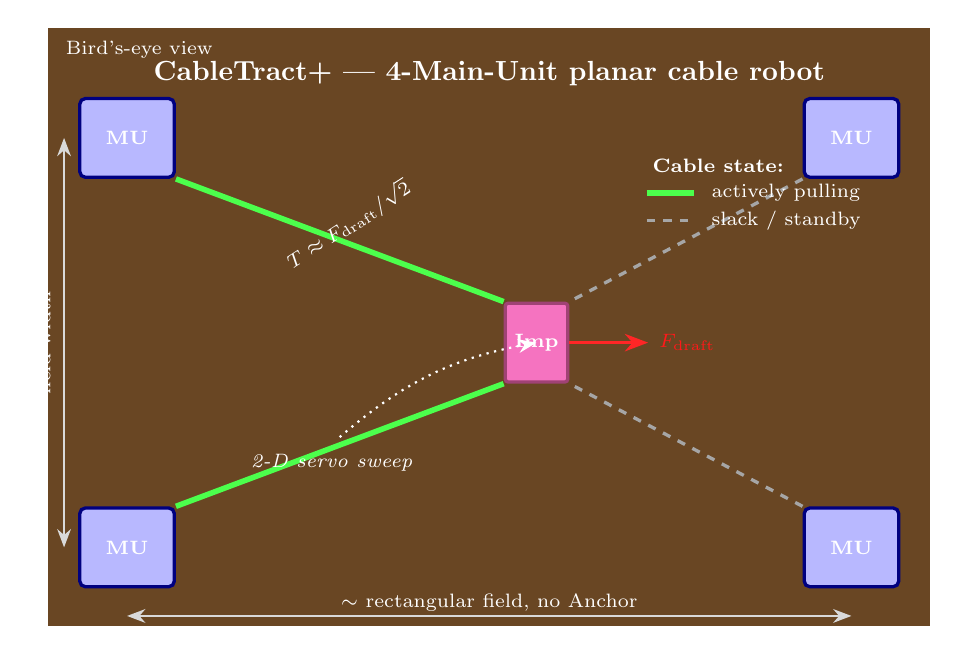
\begin{tikzpicture}[
    every node/.style={font=\footnotesize},
    field/.style={fill=brown!55!black},
    mu/.style={draw=blue!50!black, very thick, fill=blue!28, rounded corners=2pt,
               minimum width=12mm, minimum height=10mm, align=center,
               font=\scriptsize\bfseries, text=white},
    impl/.style={draw=magenta!60!black, very thick, fill=magenta!55, rounded corners=1pt,
                 minimum width=4mm, minimum height=10mm, align=center,
                 font=\scriptsize\bfseries, text=white},
    cable/.style={white, very thick},
    cableActive/.style={green!70!white, line width=2pt},
    cableSlack/.style={gray!70, very thick, dashed},
    fdraft/.style={->, >=Stealth, very thick, red!85!white},
]

% Field background
\fill[field] (-0.6,-0.6) rectangle (10.6,7.0);
\node[white, font=\scriptsize, anchor=north west] at (-0.5,6.95) {Bird's-eye view};
\node[white, font=\bfseries, anchor=north] at (5,6.7) {CableTract+ --- 4-Main-Unit planar cable robot};

% 4 corner Main Units
\node[mu] (mu_tl) at (0.4,5.6) {MU};
\node[mu] (mu_tr) at (9.6,5.6) {MU};
\node[mu] (mu_bl) at (0.4,0.4) {MU};
\node[mu] (mu_br) at (9.6,0.4) {MU};

% Implement carriage at the centre, slightly offset
\node[impl] (im) at (5.6,3.0) {Imp};

% Two ACTIVELY pulling cables (e.g. from top-left and bottom-left toward implement)
\draw[cableActive] (mu_tl.south east) -- (im.north west);
\draw[cableActive] (mu_bl.north east) -- (im.south west);

% Two slack / standby cables from the right corners
\draw[cableSlack] (mu_tr.south west) -- (im.north east);
\draw[cableSlack] (mu_br.north west) -- (im.south east);

% Geometric load split annotation at the implement
\draw[fdraft] (im.east) -- ++(1.0,0)
    node[anchor=west, red!90!white, font=\scriptsize] {$F_{\text{draft}}$};

% Per-cable tension annotation along one active cable
\node[white, font=\scriptsize, rotate=33, anchor=south]
    at ($(mu_tl.south east)!0.55!(im.north west) + (0.05,0.05)$)
    {$T \approx F_{\text{draft}} / \sqrt{2}$};

% Indicative path: implement can sweep arbitrary 2D within the rectangle
\draw[->, >=Stealth, dotted, white, thick]
    (im.center) ++(-2.5,-1.2) to[bend left=15] (im.center);
\node[white, font=\scriptsize\itshape, anchor=north]
    at (3.0,1.7) {2-D servo sweep};

% Field dimensions
\draw[<->, >=Stealth, gray!30!white, thick]
    (mu_bl.south) ++(0,-0.35) -- ($(mu_br.south)+(0,-0.35)$);
\node[white, font=\scriptsize] at (5,-0.3) {$\sim$ rectangular field, no Anchor};

\draw[<->, >=Stealth, gray!30!white, thick]
    (-0.4,0.4) -- (-0.4,5.6);
\node[white, font=\scriptsize, rotate=90, anchor=south] at (-0.45,3.0) {field width};

% Active vs slack legend (top right area)
\begin{scope}[xshift=7.0cm, yshift=4.4cm]
\node[white, font=\scriptsize\bfseries, anchor=west] at (-0.05,0.85) {Cable state:};
\draw[cableActive] (0.0,0.5) -- (0.6,0.5);
\node[white, font=\scriptsize, anchor=west] at (0.7,0.5) {actively pulling};
\draw[cableSlack] (0.0,0.15) -- (0.6,0.15);
\node[white, font=\scriptsize, anchor=west] at (0.7,0.15) {slack / standby};
\end{scope}

\end{tikzpicture}%
}
\caption{The CableTract+ variant: a planar cable-robot (\gls{cdpr}) topology~\cite{pott2018cdpr} with one Main Unit at each of the four corners of a rectangular field, replacing the single-MU + Anchor baseline. At any instant two cables (\textcolor{green!50!black}{green}) actively pull the implement carriage while the opposite two (\textcolor{gray!40!black}{grey}, dashed) hold tension at standby. Two consequences fall out: the per-round anchoring cycle disappears entirely (corner stations are set once per field --- removing the 27\,\% anchoring-energy share and most of the setup time), and each actively pulling cable carries only ${\sim}1/\sqrt{2}\approx 0.707$ of the draft, relaxing the per-cable tension and per-corner reaction --- a \emph{tension} benefit, not an energy saving (the winches jointly still deliver the full draft power). The architectural cost is paid in CAPEX --- four Main Units plus a shared energy stack at $2.20\times$ the baseline (\cref{tab:variants-numbers}).}
\label{fig:f0e}
\end{figure}

The CableTract+ variant (\cref{fig:f0e}) replaces the single Main Unit + Anchor pair with \emph{four corner Main Units}, one at each corner of a rectangular field, so that two cables can pull the carriage simultaneously toward two adjacent corners. The carriage is now servoed in two axes by the relative tensions in the four cables, so it can sweep arbitrary 2-D paths inside the rectangle rather than being constrained to a single strip per Anchor placement. This is the standard ``planar cable robot'' topology that has been studied extensively in industrial gantry contexts; the contribution here is to import it into the field as a replacement for the baseline step-and-anchor cycle.

The architectural consequences, honestly bookkept, are two. First, \textbf{the per-round anchoring cycle disappears} --- the corner stations are set once per field, so the \SI{25.3}{\Wh} anchoring-energy term and ${\approx}90\,\%$ of the per-round setup time are eliminated (\texttt{variants.py} sets the anchoring energy to zero and \texttt{setup\_overhead\_reduction = 0.9}). This is what lifts throughput to \textbf{16.5 decares/day ($1.37\times$)} and cuts energy intensity to \textbf{889 Wh/decare ($0.73\times$)}. Second, because two cables pull together at roughly orthogonal angles, \textbf{each cable carries only ${\approx}1/\sqrt{2} \approx 0.707$ of the draft load}, relaxing the per-cable tension and per-corner reaction --- the constraint that bound the baseline in the anchor envelope of \cref{sec:anchor}. We emphasise what an earlier revision got wrong: the tension split is \emph{not} an energy saving (the work done against the soil is unchanged, and the winches jointly still deliver it), and servoing two axes does not widen the implement --- the earlier revision's $2.61\times$ throughput and $0.53\times$ energy multipliers double-counted both effects and are withdrawn. CableTract+ inherits the same regen drive as the baseline.

The cost of this performance is paid in CAPEX. Four Main Units (each including its regen drive) plus the carriage and the shared battery + PV + wind + install pack cost \textbf{$2.20\times$ a single Main Unit + Anchor pair} (the multiplier sits below $4\times$ because the Anchor disappears and the energy stack is paid once): $4 \times \SI{17800}{\EUR} + \SI{2800}{\EUR} + \SI{3420}{\EUR} + \SI{1650}{\EUR} + \SI{1500}{\EUR} + \SI{4000}{\EUR} \approx \SI{85000}{\EUR}$, and the simple payback stretches from 180.3 to 287.4 months. \textbf{CableTract+ buys a $1.37\times$ throughput gain and a $0.73\times$ energy gain for $2.20\times$ the capital} --- clearly Pareto-inferior on economics, and worthwhile only where the anchoring cycle itself is the binding problem: loose-sand sites where per-strip anchoring is marginal (\cref{sec:anchor}), or calendar-time-limited large rectangular fields. On small irregular fields the four-corner geometry cannot be installed at all. For the codesigned reference scenario, the single-Main-Unit baseline is the better design point.

\subsubsection{Variant 4 --- Unidirectional drivetrain (no regen)}\label{sec:variant-norering}

The fourth configuration is the baseline with the four-quadrant regen drive removed: a plain one-way drivetrain that pulls the carriage outbound under load and tows it back at idle power, with no energy recovery. It is the \emph{cheapest} of the three (\SI{300}{\EUR} below the baseline, since the regen-capable controller is dropped) and changes nothing else about the cable architecture or the BOM. We include it to quantify exactly what making regen standard buys. As derived in \cref{sec:drivetrain}, the regen credit is a slope-averaged ${\approx}3.5\%$ effective-efficiency gain ($0.50 \to 0.518$; ${\approx}0$ on perfectly flat ground); removing it returns the one-way 0.50.

The result isolates the regen contribution and shows it is small. \textbf{Energy per decare rises only from 1\,227 to 1\,259 Wh ($1.03\times$, a slope-averaged ${\approx}2.6\,\%$ increase; ${\approx}0$ on flat ground)} when the return-leg recovery is removed --- far less than a naive ``half the round is unloaded'' argument would suggest, because the draft work is dissipated irreversibly in the soil and cannot be regenerated. \textbf{Throughput barely moves} (12.0 $\to$ 11.7) and \textbf{simple payback lengthens only from 180.3 to 183.6 months}. The case for keeping a four-quadrant drive standard therefore rests on the smooth, fast torque control it gives the depth-control loop (\cref{sec:open-risks}) and the slope-recovery upside, not on the flat-field energy saving; the unidirectional row exists to show the modest penalty of omitting it.

\subsubsection{What the variant comparison tells us}\label{sec:variants-discussion}

Three takeaways flow from \cref{tab:variants-numbers}:

\begin{itemize}[leftmargin=1.6em,itemsep=0.2em]
    \item \textbf{The anchoring cycle is the design lever the comparison exposes --- and multi-strip anchoring is the efficient way to pull it.} Both anchoring-side variants beat the baseline on energy and throughput, but at wildly different prices: CableTract+ eliminates the cycle entirely for a \SI{46.3}{\kilo\EUR} capital increment, while the beam variant recovers two-thirds of the same energy gain (and posts the table's best simple payback, $0.82\times$) for \SI{1.5}{\kilo\EUR}. On payback-per-euro the ordering is decisively multi-strip $>$ baseline $>$ CableTract+.
    \item \textbf{The baseline remains the reference because its budgets are fully verified.} The beam variant's numbers are conditional on the yaw-moment load path (frame-coupled screws, $k \le 4$) and the braked-wheel holding assumption, neither of which has been tested beyond static screening; CableTract+ additionally cannot be installed on small irregular fields. A healthy comparison keeps the conservative row as the anchor of the table.
    \item \textbf{Regen earns its place for control, not energy.} Its slope-averaged energy value is ${\approx}2.6\%$; the four-quadrant drive is standard for the depth-control torque quality (\cref{sec:v-s1}) and slope recovery.
\end{itemize}

\paragraph{Reconciling the variant table with the \cref{sec:economics} discounted payback.} The simple-payback column of \cref{tab:variants-numbers} and the discounted chain of \cref{sec:economics} answer different questions on different bases, and the full definition of the table's column is: sales price (machine CAPEX $\times 1.33$ margin) divided by \emph{fuel-only} savings at the machine's full energy-limited utilisation (${\approx}\SI{204}{\hectare\per\year}$ for the baseline --- eight times the \SI{25}{\hectare\per\year} reference of the NPV chain), with no discounting and no maintenance offset. It is an additive-buyer stress metric for comparing the three rows on one axis, not a forecast for the reference farm (at \SI{25}{\hectare\per\year} the same formula would give over 80 years). The replacement-frame chain of \cref{sec:economics} is the decision-relevant number: approximately break-even at \SI{25}{\hectare\per\year} and robustly positive above ${\sim}\SI{40}{\hectare\per\year}$. Within the table's own frame, the ordering is informative: the unidirectional design pays back \emph{later} than the baseline despite lower capex (its higher energy intensity displaces less diesel), and CableTract+ pays back much later because its capital more than doubles while its savings rise only $1.37\times$.

\subsection{Operating envelope}\label{sec:envelope}

The final question --- which the rest of the paper has been building toward --- is where in the (annual \gls{ghi} $\times$ farm size) plane CableTract is viable against diesel, and what binds when. A single point estimate at \SI{25}{\hectare\per\year} on a Mediterranean site does not generalise to \SI{1}{\hectare\per\year} on a cloudy continental site, or to \SI{1000}{\hectare\per\year} in low-\gls{ghi} France. \Cref{fig:f21} resolves both extremes at once with a 2D parameter sweep over the joint plane.

To make the sweep tractable, we calibrate a one-parameter linear \gls{pv} harvest model from the hourly site simulations of \cref{sec:energy}:
\begin{equation}\label{eq:harvest}
\text{annual\_harvest\_kWh} \;=\; \alpha \cdot \text{pv\_area\_m}^{2} \cdot \text{annual\_GHI\_kWh\_m}^{-2}\text{\_yr}^{-1},
\end{equation}
with $\alpha = 0.169$ fitted as the median across the 6 bundled sites at the codesigned \SI{15}{\meter\squared} \gls{pv}. This is intentionally a rough analytical fit, not a reproduction of the full hourly \gls{tmy} pipeline; the goal is a defensible \gls{pv} harvest as a function of annual \gls{ghi} so the envelope sweep stays in closed form.

For each cell of the (annual \gls{ghi} $\times$ farm size) grid we then compute the codesigned operating demand (energy per hectare times farm size, plus an idle-power penalty over the off-season), the harvested energy from \cref{eq:harvest}, the resulting per-hectare grid share, the \gls{npv} versus a like-for-like diesel tractor at 8\,\% over 15 years, the discounted payback, and the off-grid surplus (harvest minus demand). The sweep covers annual \gls{ghi} from 800 to \SI{2300}{\kWh\per\meter\squared\per\year} and annual operated area from \SIrange{1}{1000}{\hectare} on a log-scale --- 60 $\times$ 60 $=$ 3\,600 cells in total. The area axis (vertical in \cref{fig:f21}a) is \emph{annual operated area}, not the capacity of one machine: a single baseline unit at \SI{12.0}{decares\per day} over 170 operating days covers ${\approx}\SI{204}{\hectare\per\year}$, so the upper part of the axis ($\gtrsim$\,200\,ha) implies a multi-unit fleet, which the per-hectare economics scale to directly. Diesel is held at the \cref{sec:economics} baseline of \SI{1.40}{\EUR\per\litre} (EU 2024); a subsidised-diesel price would shift the ${\approx}\SI{40}{\hectare\per\year}$ financial threshold upward roughly in proportion to the lost fuel saving.

\begin{figure}[H]
\centering

\includegraphics[width=0.95\linewidth]{F21_operating_envelope}
\caption{CableTract operating envelope on (annual \gls{ghi} $\times$ farm size). \textbf{(a)} \emph{Annual} energy balance: yearly PV harvest minus yearly demand (green $=$ energy positive, red $=$ grid needed); an annual-surplus test, \emph{not} the hourly autonomy of \cref{tab:site-summary}. The black contour is annual breakeven. The six bundled reference sites are scattered at \SI{25}{\hectare} annual operating area. \textbf{(b)} Discounted payback (years vs diesel @ \SI{1.40}{\EUR\per\litre}, \SI{8}{\percent}, 15 yr, replacement frame) across the same 3\,600 cells. \gls{npv} is positive in 48\,\% of cells --- essentially those above ${\approx}\SI{40}{\hectare\per\year}$; below that threshold the increment does not amortise within the horizon. Under the additive frame only ${\approx}12\%$ of cells are \gls{npv}-positive.}
\label{fig:f21}
\end{figure}

Three findings flow from \cref{fig:f21}:

\begin{itemize}[leftmargin=1.6em,itemsep=0.15em]
    \item \textbf{The financial envelope is a farm-size threshold.} \gls{npv} versus diesel is positive in \textbf{48\,\%} of the 3\,600 cells --- essentially every cell above ${\approx}\SI{40}{\hectare\per\year}$ of annual operated area, at any \gls{ghi} --- and negative below it. (An earlier revision reported 100\,\% of cells positive; that result rested on the uncosted carriage, an implement-blind capex parity, and the diesel-maintenance credit surviving into the additive frame, all corrected in \cref{sec:economics}.) Under the \emph{additive} frame (full system financed, no tractor retired) only ${\approx}12\%$ of cells --- beyond a single machine's capacity --- are \gls{npv}-positive.
    \item \textbf{The energy envelope is broad.} Panel (a) is an \emph{annual} PV-harvest-minus-demand balance (not the hourly autonomy of \cref{fig:f8}; wind is excluded from the fitted harvest, a small conservatism); its breakeven contour leaves \textbf{${\approx}81\%$} of cells annual-energy-positive, with the deficit corner at large operated areas in low-\gls{ghi} climates. All six bundled reference sites at \SI{25}{\hectare} sit inside the annual-energy-positive region with comfortable surplus (lowest at Beauce, highest at Ludhiana at published \gls{ghi}). Annual surplus remains a weaker, separate claim from hourly off-grid autonomy (\cref{tab:site-summary}).
    \item \textbf{The operating envelope therefore has one financial axis and one climate axis, and they bind in different corners.} Below ${\approx}\SI{40}{\hectare\per\year}$ the economics bind everywhere; above it, the remaining question is climatic --- whether the machine can be sold as off-grid hardware (high-\gls{ghi} sites) or as grid-assisted low-carbon hardware (low-\gls{ghi} sites at large areas, where the annual energy balance also turns negative for a single energy stack). A farmer in Beauce at \SI{50}{\hectare\per\year} gets a positive \gls{npv} with an annual energy surplus but ${\approx}\SIrange{150}{300}{\hour\per\year}$ of seasonal backup; a farmer in Konya at the same area gets the same \gls{npv} \emph{and} genuine off-grid operation.
\end{itemize}

This scale-and-climate envelope is the central result of the paper.

% ====================================================================
\section{Competitor Comparison}\label{sec:competitor}
% ====================================================================

Public-domain reference numbers for the five vehicle classes named in \cref{sec:related-adjacent} (six representative machines plus CableTract) are recorded in the bundled competitor table.\footnote{\texttt{tables/competitor\_comparison.csv} in the repository.} Selected columns are reproduced in \cref{tab:competitor}.

\begin{table}[H]
\centering\small
\caption{Competitor comparison table. Competitor rows are indicative manufacturer/press figures at their own scenarios (not peer-reviewed and not directly comparable); CableTract's payback is scale-dependent (\cref{sec:npv-farmsize}: ${\approx}14$ yr at 25, 5.4 yr at 50, 2.5 yr at \SI{100}{\hectare\per\year}, replacement frame). \textsuperscript{a}Off-grid is climate-conditional (\cref{tab:site-summary}). \emph{Energy/ha} is delivered electrical energy for every row except the diesel tractor, whose \SI{120}{\kWh\per\hectare} is fuel (primary) energy from $12\,\si{\litre\per\hectare}$ at ${\approx}\SI{10}{\kWh\per\litre}$; on a useful-work basis the diesel figure is ${\approx}\SI{36}{\kWh\per\hectare}$ (\cref{sec:r-c2}). The kW column is the propulsion rating (CableTract: \SI{3}{\kilo\watt} peak winch \gls{pmsm}).}\label{tab:competitor}
\resizebox{\textwidth}{!}{%
\begin{tabular}{lllrrrrl}
\toprule
Vehicle & Form factor & Powertrain & kW & Energy/ha (kWh) & CAPEX (\si{\EUR}) & Payback (\si{\year}) & Off-grid? \\
\midrule
\textbf{CableTract codesigned}    & cable-driven 2-module & PV+wind+battery & 3.0  & \textbf{12.3} & 38\,670 & scale-dep. & \textbf{yes\textsuperscript{a}} \\
Monarch MK-V                       & 4WD tractor          & battery EV       & 55   & 52    & 85\,000 & 5--7 & no \\
FarmDroid FD20                     & autonomous robot     & onboard PV       & 0.4  & 1.5   & 75\,000 & 4--6 & yes \\
Kubota LXe-261                     & compact tractor      & battery EV       & 18   & 30    & 52\,000 & 6--8 & no \\
ecoRobotix AVO class               & solar weeder/sprayer & onboard PV+bat   & 0.6  & 0.4   & 65\,000 & 4--6 & yes \\
Na\"io Oz                          & autonomous weeder    & battery          & 2.5  & 5     & 38\,000 & 3--5 & partial \\
Conventional 80 hp diesel          & tractor              & diesel \gls{ice} & 60   & 120   & 35\,000 & ref. & no \\
\bottomrule
\end{tabular}%
}
\end{table}

CableTract occupies a distinctive cell of this table: among the compared classes it is the only architecture that \textbf{simultaneously} (a) supports light/medium primary tillage (within its codesigned envelope) and (b) is off-grid capable in the self-powered sense (climate-conditional, \cref{tab:site-summary}). Its economics, however, are scale-dependent rather than uniformly short-payback (\cref{sec:npv-farmsize}). The Monarch MK-V far exceeds it on rated power and operates at conventional speeds but is grid-dependent; FarmDroid matches it on off-grid but cannot till.

We deliberately do \emph{not} claim CableTract beats every competitor on every metric. The ecoRobotix class is more energy-efficient per hectare (\SI{0.4}{\kWh\per\hectare} vs 12.3) because it only weeds and sprays. Na\"io is cheaper. Monarch MK-V is more powerful and operates at conventional speed. And controlled-traffic farming with existing machinery (\cref{sec:related-ctf}) captures much of the trafficked-area benefit at near-zero capital. The claim is that CableTract occupies a specific cell in the feasibility space --- \emph{medium-load draft operations on ${\gtrsim}\SI{40}{\hectare\per\year}$ of annual area in high-irradiance climates, with off-grid electric energy} --- that no other vehicle in the table fills as cleanly.

% ====================================================================
\section{Results}\label{sec:results}
% ====================================================================

This section consolidates the per-figure findings of \cref{sec:methods} into a verdict against the four claims of \cref{sec:rqs} (C1--C4) plus the operating envelope; the supporting figures, tables, and derivations live in \cref{sec:methods} and are cross-referenced rather than repeated.

\subsection{C1 --- Compaction}\label{sec:r-c1}

CableTract reduces the trafficked field area by \textbf{${\approx}47\,\%$} (${\approx}27\,\%$ vs ${\approx}50\,\%$ of field area per pass) and the field-integrated $p^2$-weighted soil-stress exposure by \textbf{${\approx}39\times$} across rectangle, L-shape, and irregular-concave field classes (\cref{fig:f12}, \cref{sec:f12}); both C1 thresholds (${\geq}40\,\%$ area, ${\geq}20\times$ exposure) are met. The reductions are uniform across field shape because they are geometric: the carriage lays one \SI{0.4}{\meter} roller track per \SI{1.5}{\meter} swath at \SI{31}{\kilo\pascal}, versus the tractor's \SI{0.9}{\meter} of tyre track per \SI{1.8}{\meter} gauge at \SI{143}{\kilo\pascal}. The architecture's distinctive gain is the \emph{pressure} (below the ${\sim}\SI{50}{\kilo\pascal}$ subsoil criterion at structural weight; ${\approx}\SI{52}{\kilo\pascal}$ during heavy-downforce tillage passes, \cref{sec:compaction}), while the trafficked-area discipline is comparable to good \gls{ctf} (\cref{sec:related-ctf}). The per-running-gear contact-energy index ($\sum p^2 A_{\text{patch}}$, $73\times$) is reported separately and should not be multiplied by the area reduction. All values are computed from open published static contact-pressure values without dynamic \gls{fem} calibration, and we do not claim any index maps linearly onto soil damage or yield.

\subsection{C2 --- Energy}\label{sec:r-c2}

The codesigned reference (regen default, anchoring charged) operates at \textbf{\SI{1227}{\Wh\per\decare} (\SI{12.3}{\kWh\per\hectare})} of delivered electrical energy, of which ${\approx}27\%$ is the anchoring cycle (\cref{sec:anchoring-energy}). An \SI{80}{hp} \gls{wd} diesel comparator burns ${\approx}\SI{12}{\litre\per\hectare}$ on the same operations~\cite{asabe-d497,siemens1999machinery} --- ${\approx}\SI{120}{\kWh\per\hectare}$ of \emph{primary fuel} energy, of which only ${\sim}30\text{--}35\%$ reaches the drawbar as useful work (${\approx}\SI{36}{\kWh\per\hectare}$). CableTract's delivered electricity is \textbf{$2.9\times$ below the comparator's estimated drawbar work} (a deliberately mixed basis, conservative in the comparator's favour --- CableTract's own drawbar output is ${\approx}\SI{4.7}{\kWh\per\hectare}$, so the strict drawbar-to-drawbar ratio is ${\approx}7.7\times$) and ${\sim}10\times$ below its primary-fuel energy; most of the primary-energy factor is the diesel engine's thermal-conversion loss, generic to any electric drivetrain. The architectural advantage decomposes into three levers (a unidirectional drivetrain gives \SI{1259}{\Wh\per\decare}, only ${\sim}2.6\%$ more; the return-leg recovery is a small, slope-driven effect, \cref{sec:variant-norering}):

\begin{itemize}[leftmargin=1.6em,itemsep=0.1em]
    \item \textbf{Co-designed implements} (\cref{fig:f4,fig:f5}). The median of the per-implement P50 drafts drops from ${\approx}\SI{6.2}{\kilo\newton}$ (conventional library) to ${\approx}\SI{2.5}{\kilo\newton}$ (codesigned library), a factor of ${\approx}\,2.5$, via narrower widths, slower speeds, and shallower depths (with the operating-point caveats of \cref{sec:codesign}).
    \item \textbf{No dead-weight transport.} The draft term $F_d L$ is 72\,\% of the round work and the in-field work ($F_d L + F_i L$) 96\,\% (\cref{sec:pass-model}); the diesel comparator's body-repositioning force, paid over the whole field rather than once per strip, dwarfs this on every operation.
    \item \textbf{Decomposed drivetrain} (\cref{fig:f3}). A premium drivetrain ($\eta = 0.74$) reduces continuous motor power from \SI{1.80}{\kilo\watt} to \SI{1.22}{\kilo\watt} at the reference load and sizing speed. The codesigned reference uses a \SI{2}{\kilo\watt} continuous / \SI{3}{\kilo\watt} peak \gls{pmsm}, with heavy implements run derated (\cref{sec:motor}).
\end{itemize}

The energy story is therefore not ``CableTract has a magic motor'' but ``CableTract pulls a lighter implement, slower, without a 4-tonne body --- and converts electricity instead of burning diesel --- while paying a new, previously hidden cost: re-anchoring thirteen ground screws every strip.'' The architectural levers give the ${\sim}2.9\times$ advantage against the comparator's drawbar work; the diesel-to-electric conversion step accounts for the further factor that lifts the primary-energy ratio to ${\sim}10\times$.

\subsection{C3 --- Off-grid feasibility}\label{sec:r-c3}

Per-site median throughput on harvested energy alone ranges from \textbf{6.5 to 9.3 \si{decares\per day}} at the codesigned hardware (\SI{15}{\meter\squared} \gls{pv}, \SI{9}{\kWh} battery; \cref{tab:phase3-pcts}). Every site runs grid-free through its own brightest week (\cref{fig:f7}). Under the seasonal 170-day duty cycle the annual readout (\cref{tab:site-summary}) is: \textbf{Konya \SI{58}{\hour\per\year} of grid support (off-grid)}; Des Moines, Palencia, São Paulo, and Ludhiana \SIrange{150}{211}{\hour\per\year} (near-off-grid, \SIrange{96}{98}{\percent} of in-season energy harvested on-board); Beauce \SI{282}{\hour\per\year}. Full autonomy ($<\!\SI{100}{\hour\per\year}$) is reachable at every site by ${\approx}\SIrange{27}{30}{\meter\squared}$ of \gls{pv} (\cref{fig:f8}).

The off-grid claim is \textbf{climate-conditional, not categorical --- but no bundled site is categorically infeasible}. A CableTract sold into Konya is genuinely off-grid hardware; sold into Beauce it is a low-carbon machine with ${\approx}\SI{255}{\kWh\per\year}$ of seasonal backup (or a larger panel). An earlier revision, which applied the work duty 365 days per year, concluded Beauce was infeasible off-grid at any hardware scale; that conclusion is withdrawn (\cref{sec:phase3-findings}).

\subsection{C4 --- Economics}\label{sec:r-c4}

In the replacement frame (machine capex increment \SI{3670}{\EUR}, implement sets netted), the economics are \textbf{scale-conditional}: \gls{npv} vs diesel at 8\,\% is \textbf{\SI{-1724}{\EUR}} at the \SI{25}{\hectare\per\year} reference (cost-neutral within parameter uncertainty), crosses zero near \textbf{\SI{40}{\hectare\per\year}} at all three tested discount rates, and reaches \textbf{\SI{+9061}{\EUR}} at \SI{100}{\hectare\per\year} (payback \SI{2.5}{\year}; \cref{fig:f16}, \cref{sec:npv-farmsize}). For an additive buyer financing the full \SI{48170}{\EUR} system, the \SI{25}{\hectare\per\year} NPV is ${\approx}\SI{-61}{\kilo\EUR}$ and no single machine reaches break-even within its own capacity. The tornado (\cref{fig:f14}) shows the reference sits close enough to zero that most single inputs can flip its sign, with the used-tractor price and the maintenance basis the largest swings.

Lifecycle CO\textsubscript{2} at \SI{25}{\hectare\per\year} is \textbf{\SI{17.0}{\kilogram\per\hectare\per\year}}, against \textbf{32.5} for the diesel reference and \textbf{27.9} for a Monarch-class electric tractor (\cref{fig:f17}) --- a $1.9\times$ improvement over diesel, on the operational side, independent of grid decarbonisation.

The operating envelope of \cref{fig:f21} integrates both: \gls{npv} is positive in \textbf{48\,\%} of the 3\,600 cells of the (annual \gls{ghi} $\times$ farm size) sweep --- essentially every cell above ${\approx}\SI{40}{\hectare\per\year}$ --- and ${\approx}81\%$ of cells are annual-energy-positive. Under the additive frame the \gls{npv}-positive region shrinks to ${\approx}12\%$ of cells.

The Sobol decomposition (\cref{fig:f13}) confirms that no single parameter dominates the throughput variance (top contributor $\gls{sobolt} \approx 0.25$); the economics, by contrast, are genuinely sensitive at the reference scale, which is why we frame them as ``parity at \SI{25}{\hectare\per\year}, robustly positive from ${\sim}\SI{40}{\hectare\per\year}$'' rather than favourable everywhere.

\subsection{Operating envelope}\label{sec:r-envelope}

The central result of the paper: the envelope has \textbf{one financial axis and one climate axis}. In the replacement frame the codesigned CableTract is \gls{npv}-positive in 48\,\% of the 3\,600 cells of the (annual \gls{ghi} $\times$ farm size) sweep --- essentially every cell above ${\approx}\SI{40}{\hectare\per\year}$ of annual operated area, at any irradiance --- and negative below that threshold everywhere. Above the threshold, the remaining question is climatic: ${\approx}81\%$ of cells are annual-energy-positive (distinct from, and weaker than, the hourly off-grid readout of \cref{sec:r-c3}), with the deficit corner at large areas in low-\gls{ghi} climates.

CableTract therefore follows the \emph{usual} clean-energy hardware story --- it pays back at scale, not everywhere --- with one genuine distinction: at and above its economic threshold it can also be energy-self-sufficient in high-irradiance climates. The open questions are the farm-size threshold's sensitivity to used-tractor prices and maintenance bases (\cref{sec:tornado}), and where the machine can be sold as \emph{off-grid} rather than grid-assisted hardware (\cref{tab:site-summary}).

\subsection{Architectural variants}\label{sec:r-pareto}

The variant comparison in \cref{tab:variants-numbers,fig:f20} runs four configurations on the same parameter set: the codesigned baseline (regen default), multi-strip anchoring (beam + travelling sheave, $k=4$), CableTract+ (4-Main-Unit planar cable robot), and a unidirectional drivetrain (no regen). \textbf{Multi-strip anchoring is the stand-out row}: 14.5 decares/day ($1.21\times$), \SI{974}{\Wh\per\decare} ($0.79\times$), and the table's best simple payback ($0.82\times$) for a \SI{1.5}{\kilo\EUR} beam-and-trolley increment --- conditional on the yaw-moment load path that limits it to $k=4$ in frame-coupled medium-dense soil ($k=2$ in loose sand). CableTract+ reaches $1.37\times$ throughput at $0.73\times$ energy by eliminating the anchoring cycle entirely, but at $2.20\times$ CAPEX (\SI{84997}{\EUR}), stretching simple payback to 287.4 months. Dropping regenerative braking raises energy intensity by only ${\approx}2.6\%$ for a \SI{300}{\EUR} saving; the four-quadrant drive is kept standard for depth-control torque quality and slope recovery. The comparison's lesson is that the anchoring cycle (27\,\% of energy, ${\approx}30\pm10\,\%$ of time) is the architecture's highest-leverage design margin --- and that most of it can be recovered with hardware costing 3\,\% of the CableTract+ increment, pending load-path verification.

% ====================================================================
\section{Higher-fidelity verification studies}\label{sec:verification}
% ====================================================================

The screening model of \cref{sec:methods} lumps each subsystem into a reduced-order form fit for a feasibility envelope. To stress-test the five places a sceptical reviewer is most likely to press --- the robustness of the co-design lever, the anchor capacity, the depth-control loop, the cable safety surface, and the tillage draft --- we built five purpose-specific higher-fidelity models: a full propagation of the co-design sweep, a nonlinear $p$--$y$ Winkler anchor model, a closed-loop multibody-cable depth-control co-simulation, a finite-difference cable-safety model, and a soft-sphere discrete-element (DEM) soil--tool model. These do \emph{not} replace a prototype (\cref{sec:open-risks} remains in force); they bound each risk more tightly than the screening model, and where warranted they revise a number or a framing. Every study is deterministic and reproducible from the open pipeline (\texttt{scripts/run\_phase8}--\texttt{12}, with unit tests), and each is validated against an analytic limit before it is trusted.

\subsection{Co-design robustness (S4)}\label{sec:v-s4}

The case leans on the co-designed library cutting per-pass draft substantially --- a model prediction, not a measurement (the sweep's reference-point ratio is $1800/5250 = 0.34\times$ against the speed-adjusted conventional median; the library median-of-ratios is $0.37\times$, \cref{tab:codesigned-library} --- two related but distinct statistics). We ask the reviewer's question directly: if co-design under-delivers, how much survives? Sweeping the achieved reference draft from the codesigned point (\SI{1.8}{\kilo\newton}) up to the speed-adjusted conventional median (\SI{5.25}{\kilo\newton}) and propagating every level through the \emph{full} deterministic pipeline (\cref{fig:f22}), the energy intensity and off-grid throughput degrade smoothly (at a $0.61\times$ achieved ratio, \SI{1227}{\Wh\per\decare} rises to ${\approx}\SI{1721}{\Wh\per\decare}$ and daily throughput falls from ${\approx}12.0$ to ${\approx}8.1$ decares/day), and the required screw count rises. The off-grid replacement-frame \gls{npv} is exactly invariant --- but we state plainly that this is \emph{structural}, not an empirical robustness discovery: with zero grid share and a fixed \SI{25}{\hectare\per\year} workload (which even the degraded throughput covers: $8.1 \times 170 = \SI{138}{\hectare\per\year}$ capacity), no draft-dependent cost term exists in that frame. The genuine sensitivity finding is that the energy and off-grid claims degrade smoothly with a co-design shortfall while the anchor envelope tightens.

\begin{figure}[H]
\centering

\includegraphics[width=0.95\linewidth]{F22_codesign_sensitivity}
\caption{Co-design lever sensitivity (S4). As the achieved reference draft rises from the codesigned point (\SI{1.8}{\kilo\newton}, a $0.34\times$ ratio against the speed-adjusted conventional median) toward that median, (a) energy per decare and (b) off-grid throughput degrade smoothly and (c) the required screw count climbs; (d) shows the additive-frame simple payback stretching with the shortfall, while the off-grid replacement-frame \gls{npv} is structurally draft-invariant (annotation; see text).}
\label{fig:f22}
\end{figure}

\subsection{Anchor lateral capacity from a nonlinear \texorpdfstring{$p$--$y$}{p-y} model (S7)}\label{sec:v-s7}

\Cref{sec:anchor} deliberately bracketed the per-auger lateral capacity between two literature references (\SI{400}{\newton} Qureshi~\cite{khand2024helical}, \SI{2}{\kilo\newton} Magnum~\cite{magnum2024fixed}) rather than picking one. Here we replace that ``have-it-both-ways'' gap with a single, internally derived nominal. We solve the Euler--Bernoulli beam-column on a nonlinear elastic (Winkler) foundation, $EI\,y'''' = -p(y,z)$, with the API RP 2A~\cite{api2014rp2a} / Reese~\cite{reese1974analysis} sand $p$--$y$ curves $p = A\,p_u\tanh(kzy/A p_u)$ (coefficients after Murchison \& O'Neill~\cite{murchison1984evaluation}), as a nonlinear boundary-value problem (finite differences $+$ Newton) for the lateral capacity at the IBC 2021 \SI{1}{inch} (\SI{25.4}{\milli\meter}) head-deflection serviceability limit, free- and fixed-head, with a \(3\times3\) cluster handled by row $p$-multipliers (Mokwa~\cite{mokwa1999resistance}; Reese \& Van Impe~\cite{reese2011single}). For a \SI{73}{\milli\meter} steel shaft embedded \SI{2}{\meter}, the single-pile serviceability capacity is \SI{4.8}{\kilo\newton} (loose, free-head) to \SI{16.8}{\kilo\newton} (medium-dense, fixed-head); the group efficiency is \(0.50\), giving a derived per-auger \emph{working} nominal of \SIrange{1.6}{2.3}{\kilo\newton} at a safety factor of \(1.5\). This brackets the Magnum \SI{2}{\kilo\newton} datasheet value and sits above the conservative \SI{400}{\newton} loose-sand floor (which the model now reads as a deliberately pessimistic lower bound, not a co-equal reference). The linear small-deflection limit reproduces the Het\'enyi~\cite{hetenyi1946beams} closed form $y_0 = H/(2\beta^3 EI)$ to within \SI{0.03}{\percent} (\cref{fig:f28}).

\begin{figure}[H]
\centering

\includegraphics[width=0.95\linewidth]{F28_anchor_py}
\caption{Ground-screw lateral capacity from the nonlinear $p$--$y$ Winkler model (S7), at the installed \SI{1.0}{\meter} $\times$ \SI{60}{\milli\meter} geometry: (a) API/Reese sand $p$--$y$ curves; (b) head pushover with the IBC \SI{1}{inch} serviceability capacity marked; (c) derived per-screw capacity versus the cited Qureshi/Magnum references; (d) screw count versus the draft the anchor must hold, for the derived nominal against the literature bracket.}
\label{fig:f28}
\end{figure}

\textbf{Design decision: the \(9\)-screw Anchor is retained, with head fixity as the load-bearing condition.} At the codesigned P90 of \SI{3.0}{\kilo\newton}, the frame-coupled (fixed-head) nominal carries the load with ${\gtrsim}5\times$ margin on 9 screws, while under the pessimistic free-head loose-sand reading the cluster sits at its envelope (10 screws required at \SI{374}{\newton} vs 9 installed). The design therefore leans on the screws being \emph{rigidly coupled to the Anchor frame} --- a realistic condition for a bolted drive coupling, but one a prototype must verify under cyclic load, and the frame must also resist the resulting head moments (the sheave-height overturning couple of \cref{sec:anchor} adds axial push--pull across the cluster that this lateral-only model does not cover). The screws carry no throughput penalty beyond the anchoring cycle already charged in \cref{sec:anchoring-energy}. On rake: screws raked toward the load would resist through axial helix pull-out rather than shaft bending; for shallow single-helix screws in loose sand the uplift capacity is not necessarily higher than the lateral value, so we do not claim rake as a free margin.

\subsection{Closed-loop tilling-depth control (S1)}\label{sec:v-s1}

\Cref{sec:open-risks} names the depth-control loop the single largest unresolved risk. We give it a closed-loop co-simulation. A planar lumped-mass cable (axial Hookean springs $+$ gravity) reproduces the \cref{sec:catenary} catenary sag to \SI{0.0}{\percent}, the taut-string first natural frequency $f_1 = \tfrac{1}{2L}\sqrt{T/\mu}$ to \SI{0.03}{\percent}, and conserves energy in undamped free vibration to \SI{0.008}{\percent}. It yields the cable's vertical point stiffness at midspan, ${\approx}4T/L \approx \SI{144}{\newton\per\meter}$ --- some three orders of magnitude softer than a gauge wheel on firm soil (${\sim}\SI{3e5}{\newton\per\meter}$), confirming quantitatively the \cref{sec:tension-balance} claim that \emph{the gauge wheel, not the cable, sets depth}. We then drive a reduced vertical plant (carriage mass, a unilateral gauge-wheel ground contact, and a bandwidth- and rate-limited down-pressure actuator) with three programmed disturbances --- a buried-stone impulse, a hardpan step, and a moisture ramp --- under a tuned PID and an offset-free model-predictive controller (a self-contained box-constrained QP), against a heavy-tractor benchmark.

\begin{figure}[H]
\centering
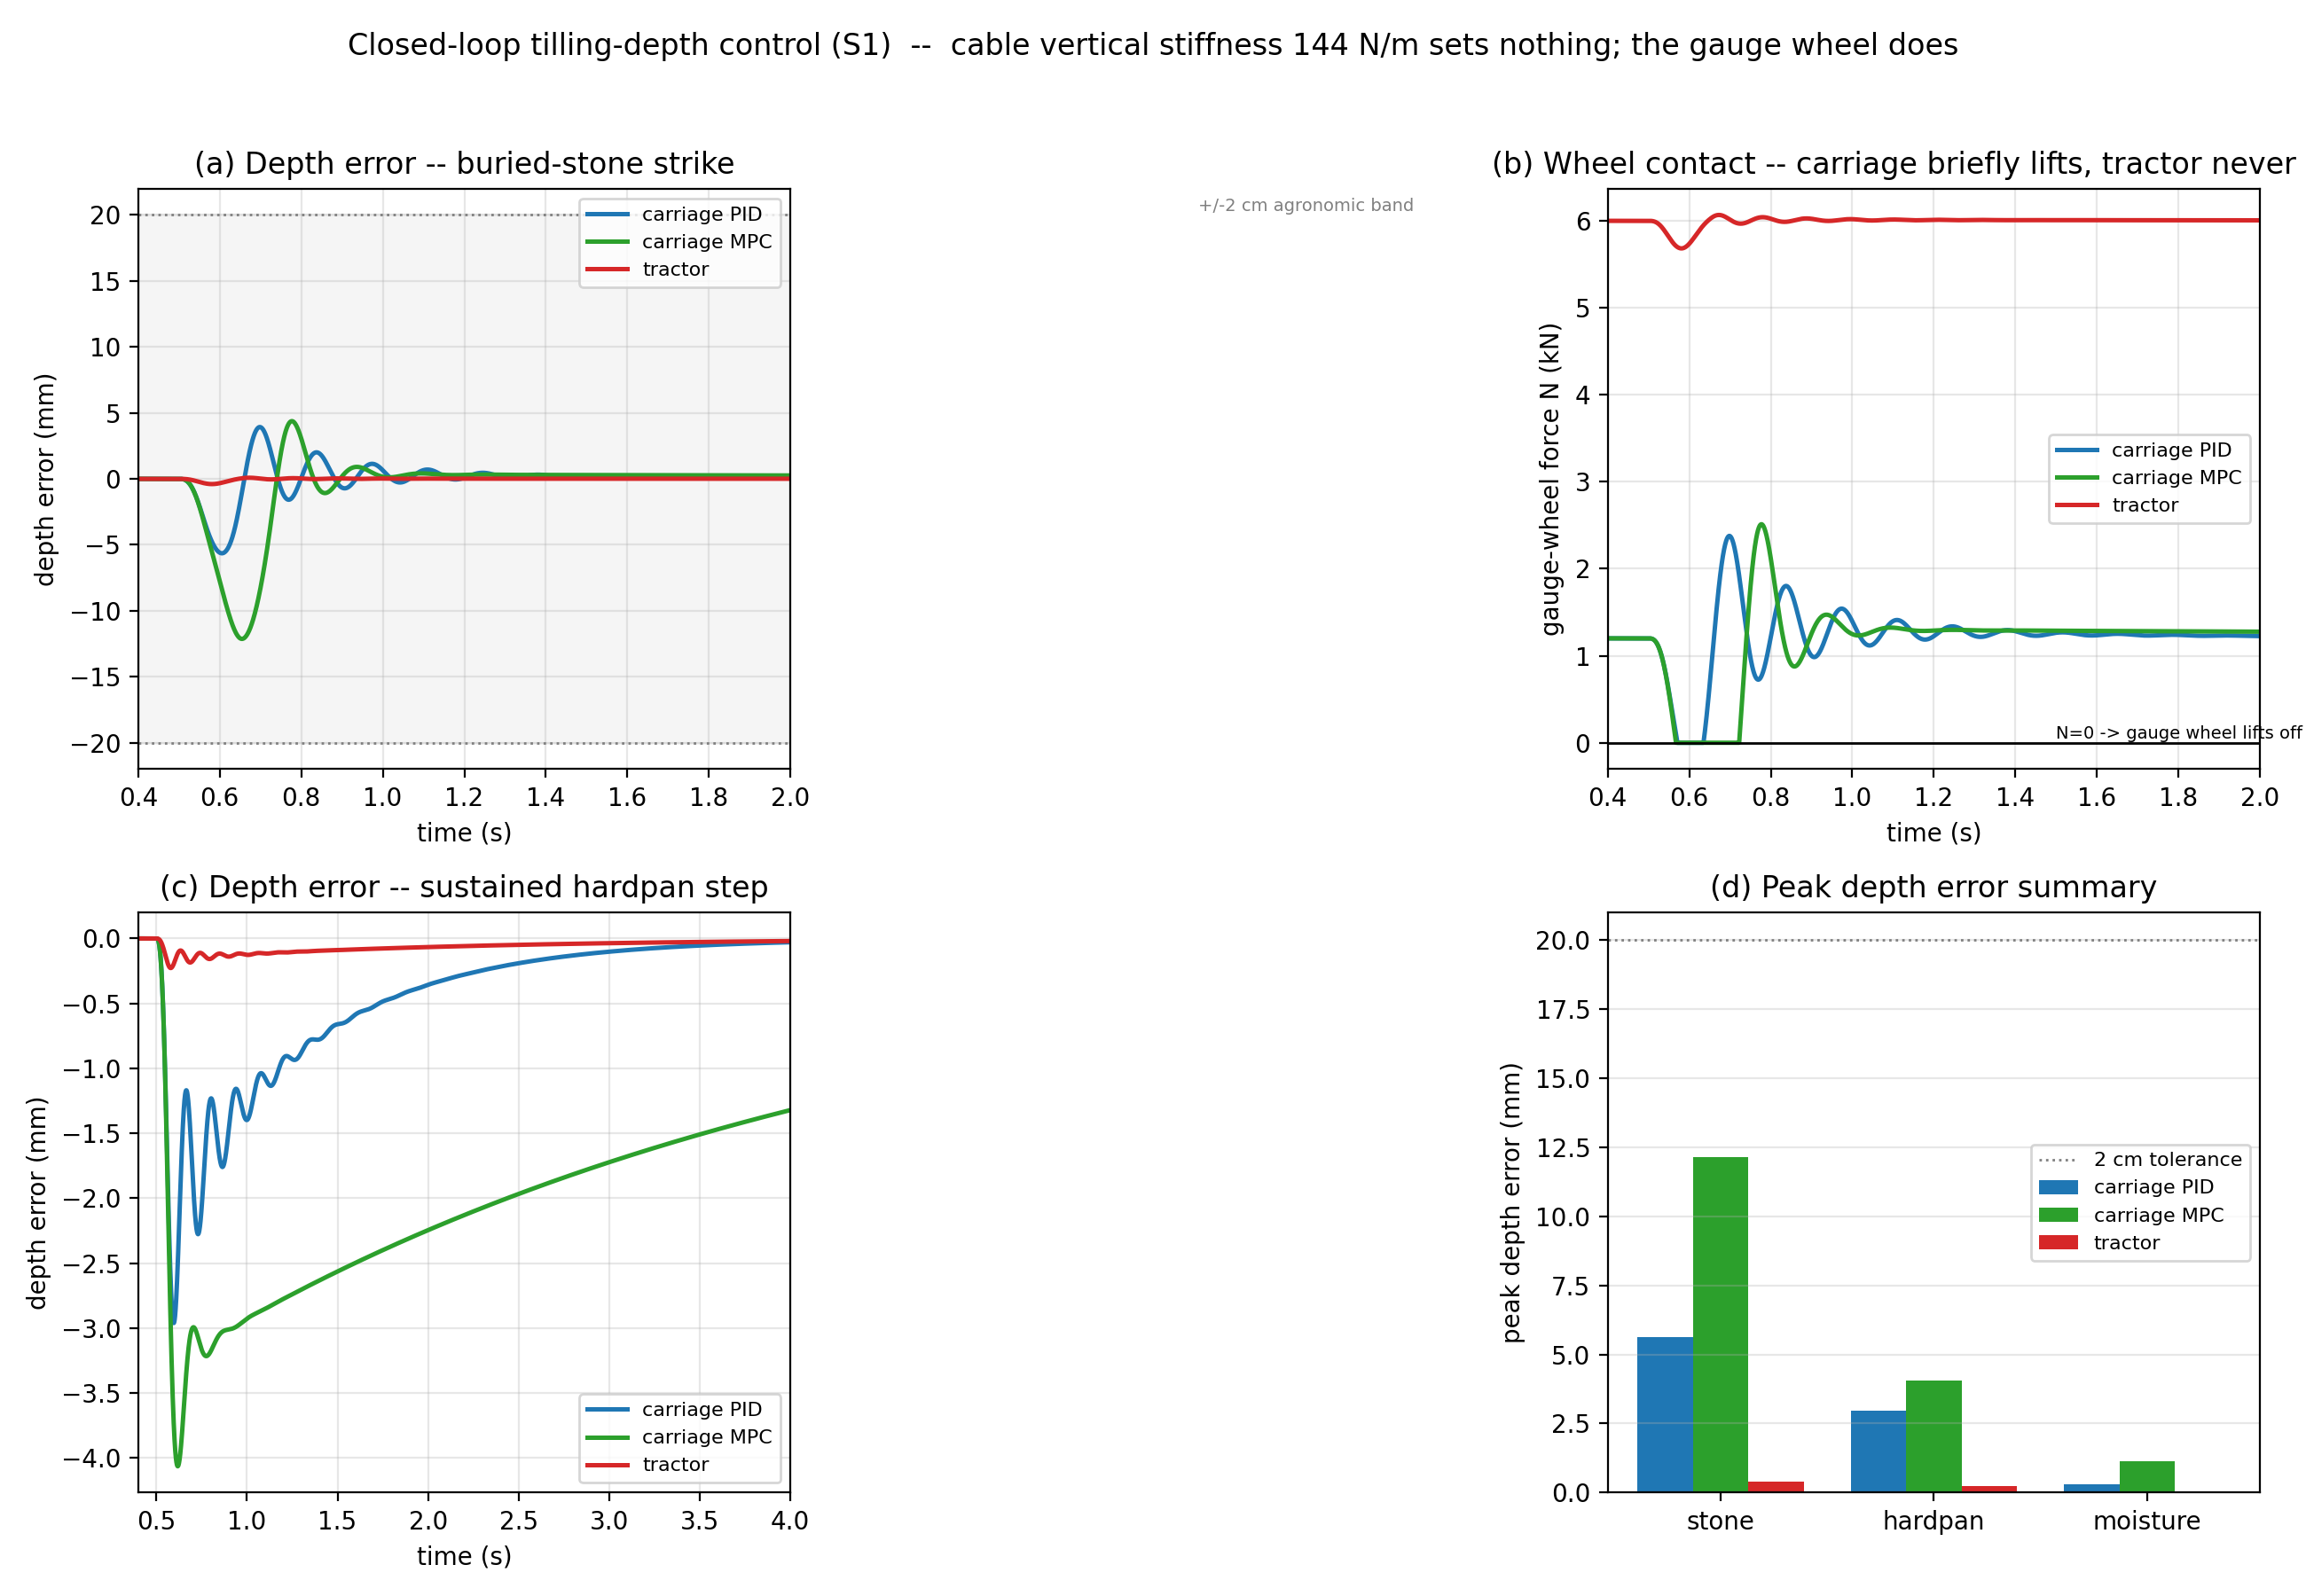
\includegraphics[width=0.95\linewidth]{F23_depth_control}
\caption{Closed-loop depth control (S1). Depth error and gauge-wheel contact force for the light cable carriage (PID and MPC) versus a heavy tractor under a buried-stone strike and a hardpan step; all controllers hold the \(\pm\SI{2}{\centi\meter}\) agronomic tolerance, but the light carriage's gauge wheel briefly unloads (\(N\!\to\!0\)) where the heavy tractor's never does.}
\label{fig:f23}
\end{figure}

All three controllers hold the depth error inside the \(\pm\SI{2}{\centi\meter}\) agronomic tolerance for every disturbance. The heavy tractor never lifts off (peak error \SI{0.4}{\milli\meter}; contact force stays ${\sim}\SI{5.7}{\kilo\newton}$). The light carriage holds depth too (PID peak \SI{5.6}{\milli\meter} on the stone strike) but its gauge wheel \emph{briefly lifts off} (${\leq}\SI{0.15}{\second}$) when the transient lift exceeds the steady wheel reserve faster than the actuator can respond. The feasibility envelope over the down-pressure reserve and actuator bandwidth (\cref{fig:f24}) gives the design specification: a steady down-pressure reserve of ${\approx}\SI{1.75}{\kilo\newton}$ at an actuator bandwidth ${\geq}\SI{5}{\hertz}$ eliminates gauge-wheel lift-off through a \SI{1.5}{\kilo\newton} stone strike. The honest reading is that depth control is \emph{feasible but must be engineered}: unlike a tractor, which holds depth for free with several tonnes of inertia, the cable carriage must carry an active down-pressure reserve, which trades against compaction (\cref{sec:compaction}). This narrows the open risk but does not close it --- the quarter-scale soil-bin bench rig of \cref{sec:open-risks} remains the right next step.

\begin{figure}[H]
\centering
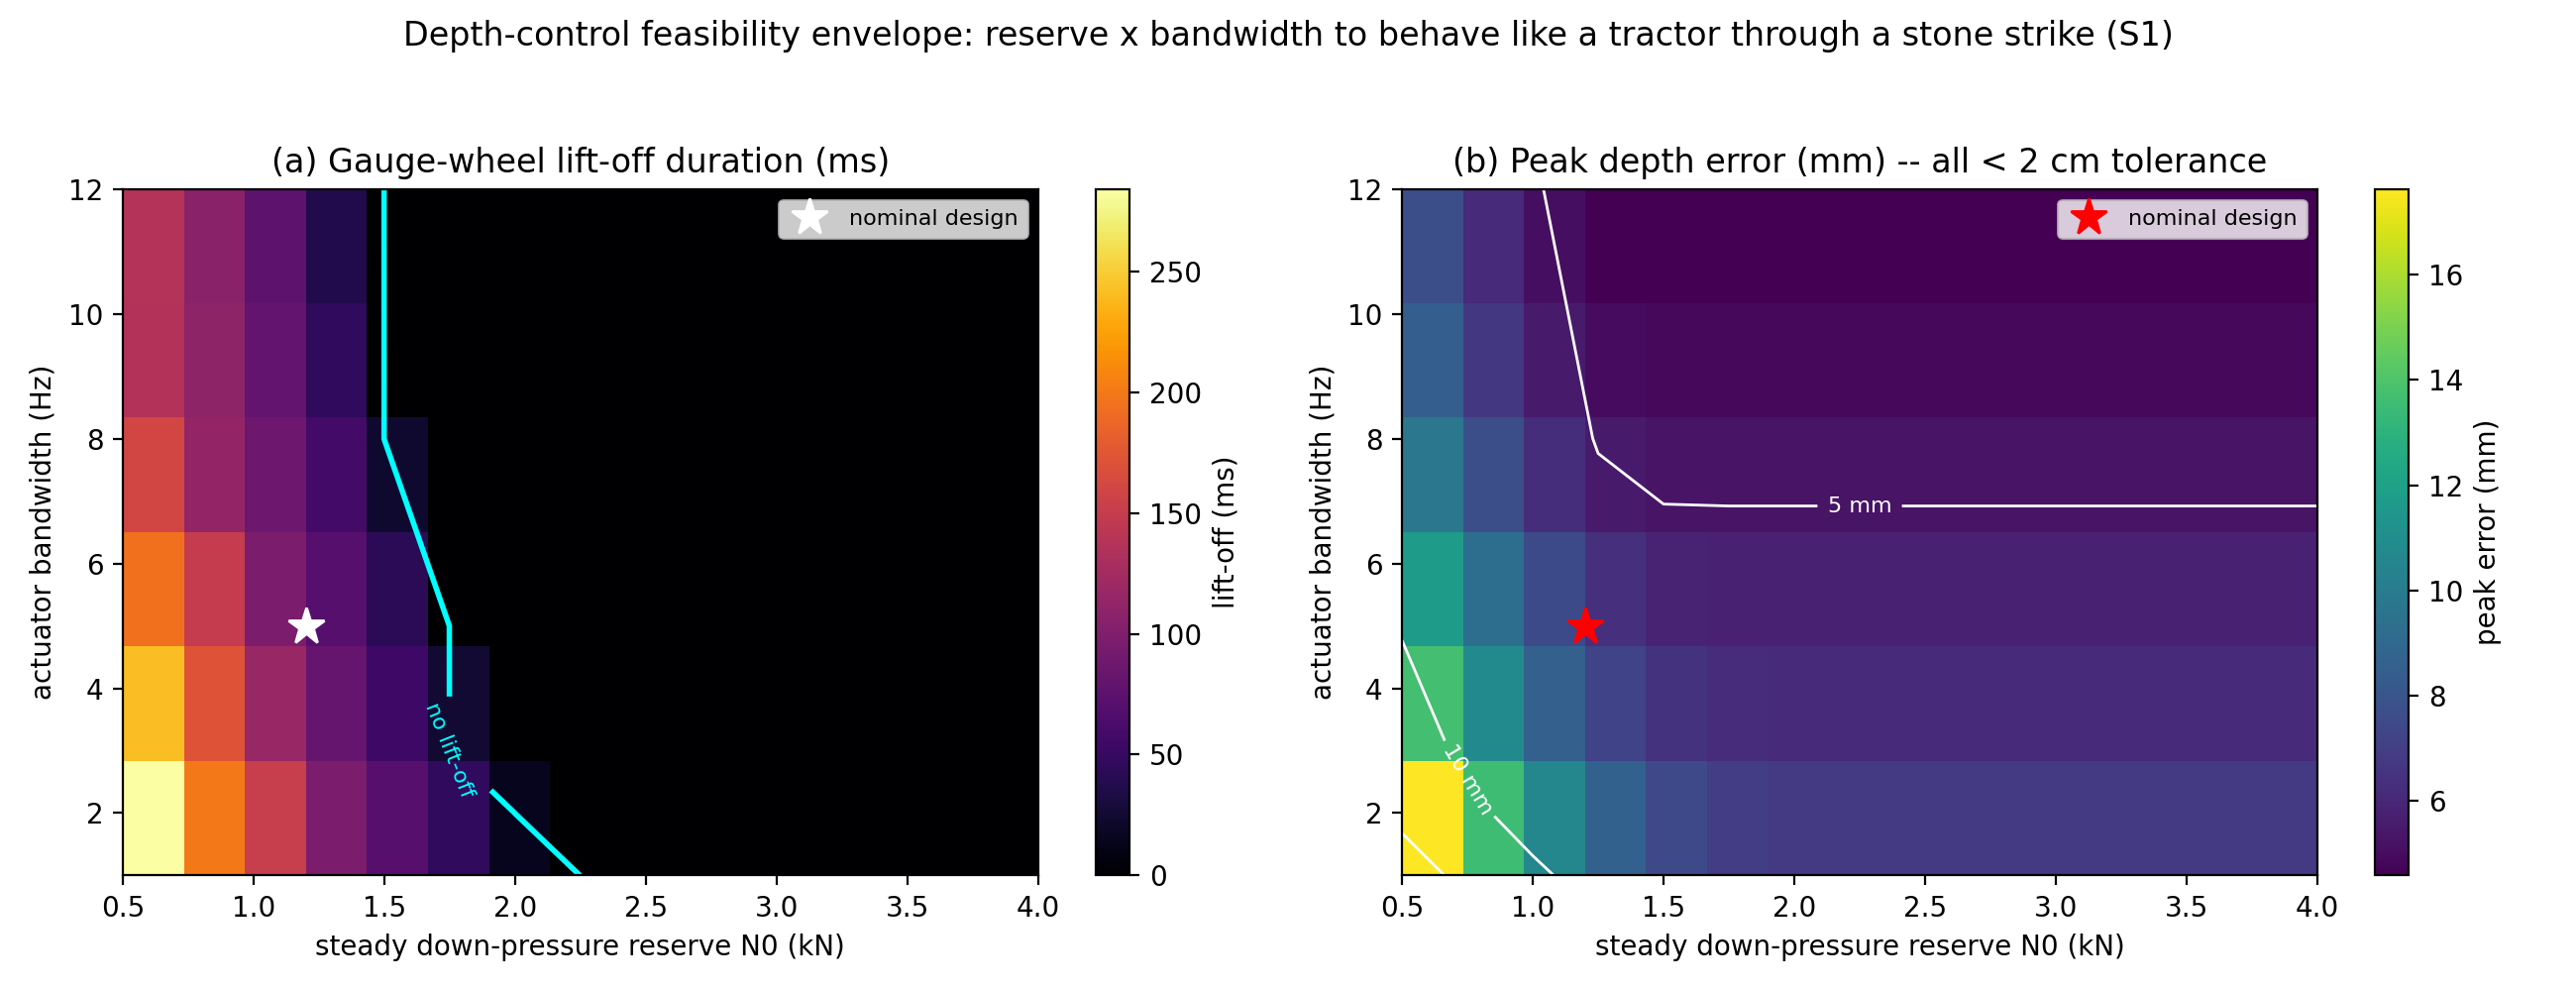
\includegraphics[width=0.95\linewidth]{F24_stability_envelope}
\caption{Depth-control feasibility envelope (S1): gauge-wheel lift-off duration (a) and peak depth error (b) over the steady down-pressure reserve $N_0$ and the actuator bandwidth. A reserve of ${\approx}\SI{1.75}{\kilo\newton}$ at ${\geq}\SI{5}{\hertz}$ removes lift-off in a \SI{1.5}{\kilo\newton} stone strike; peak depth error stays within the \(\pm\SI{2}{\centi\meter}\) tolerance throughout.}
\label{fig:f24}
\end{figure}

\subsection{Cable safety and durability (S2)}\label{sec:v-s2}

\Cref{sec:open-risks} flags the cable as an unquantified safety surface with no replacement schedule in the \gls{bom}. We address both with three sub-models (\cref{fig:f25}). \textbf{Snap-back recoil:} the axial release velocity of a suddenly-freed tensioned end is $v = T/\sqrt{EA\,m'}$, and the \emph{lighter synthetic recoils faster} at any given tension because of its much lower mass per length. At the \emph{operating} tension (P50 \SI{1.8}{\kilo\newton}) the model gives Dyneema ${\approx}\SI{6.3}{\meter\per\second}$ (\SI{22}{\joule}) versus steel ${\approx}\SI{1.4}{\meter\per\second}$ (\SI{6}{\joule}) --- below the ${\approx}\SI{79}{\joule}$ projectile-injury guideline the model carries. At fault-condition tensions, however (a snagged implement or over-tension event approaching the rated working-load limit of ${\approx}20\%$ of breaking load), Dyneema recoil reaches ${\approx}\SI{25}{\meter\per\second}$ with kinetic energy well past the guideline, so synthetic rope is \emph{not} inherently safer for snap-back despite its higher break load, and an exclusion zone during tensioned operation --- sized for the fault case, not the nominal --- remains a hard requirement whose autonomous enforcement (intrusion detection, safety-rated stops, conformity with agricultural autonomous-machinery frameworks) is uncosted here (\cref{sec:open-risks}). A finite-difference transverse-wave solver validates the wave speed $c = \sqrt{T/\mu}$ to \SI{0.03}{\percent}. \textbf{Bending-over-sheave fatigue:} a Feyrer-type model~\cite{feyrer2015wireropes} shows that at the working load of only ${\approx}5\%$ of break load the bending-fatigue life is effectively unbounded (${\sim}10^4$ yr at the design $D/d=25$); replacement is therefore governed by UV and abrasion at ${\approx}\SI{8}{\year}$, which we add as a new operating-cost and life-cycle line (${\approx}\SI{60}{\EUR\per\year}$ steel, ${\approx}\SI{180}{\EUR\per\year}$ Dyneema; a few \si{\kilogram} CO\textsubscript{2}/yr) in \cref{sec:economics}. \textbf{Aeroelastic stability:} the long taut cable has a dense modal spectrum, so vortex-induced vibration~\cite{blevins1990flow} is possible at the bundled site winds and a deployed cable would need dampers; the Den Hartog~\cite{denhartog1956mechanical} galloping onset for an iced section (\SIrange{0.4}{0.9}{\meter\per\second}) sits below the site winds, so the cable should be de-tensioned in icing conditions --- a constraint largely mitigated by growing-season-only operation.

\begin{figure}[H]
\centering
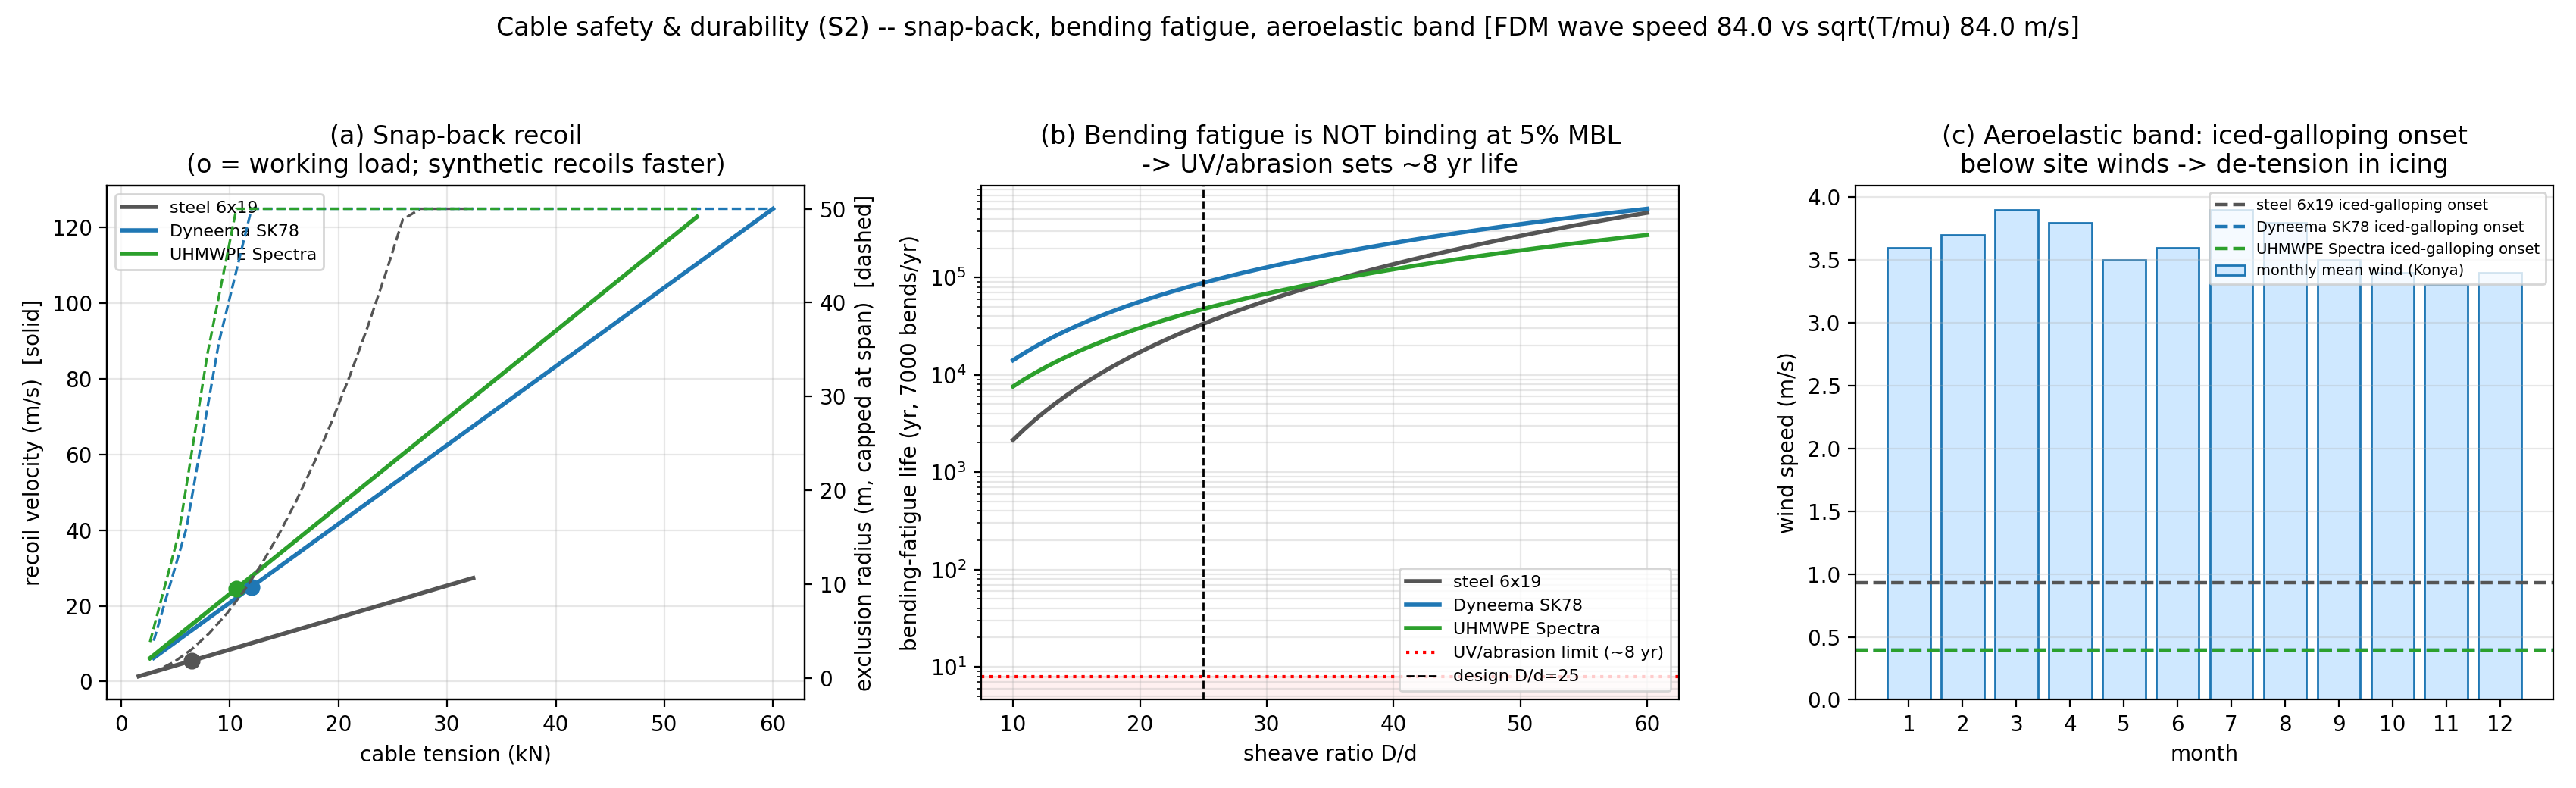
\includegraphics[width=0.95\linewidth]{F25_cable_safety}
\caption{Cable safety and durability (S2): (a) snap-back recoil velocity and exclusion radius versus tension for steel, Dyneema, and UHMWPE; (b) bending-fatigue life versus sheave ratio $D/d$, showing the working load is UV/abrasion-limited, not fatigue-limited; (c) aeroelastic band --- iced-galloping onset against the bundled monthly mean winds.}
\label{fig:f25}
\end{figure}

\subsection{Soil--tool DEM of the co-designed implements (S3)}\label{sec:v-s3}

Finally we test the co-design draft prediction and the shallow-narrow-versus-deep-wide tilth question with a three-dimensional soft-sphere DEM (Hertz--Mindlin contacts, ${\approx}8000$ particles), cross-checked against an analytic McKyes--Godwin~\cite{mckyes1985soil} / Reece~\cite{reece1965fundamental} soil-cutting wedge (Godwin \& Spoor~\cite{godwin1977soil}). The bed packs to a realistic \emph{settled} (untilled seedbed) bulk density of \SI{1625}{\kilogram\per\meter\cubed}, and the drag force rises with tool depth, width, and inter-particle friction as expected; the field-cohesion wedge, extrapolated to field depth, is of the same order as the codesigned primary-tillage drafts (\cref{fig:f26}; the comparison is order-of-magnitude only, since the wedge is a single tine at greater depth than the library's shallow operating points). On tilth (\cref{fig:f27}), a shallow-narrow co-designed pass disturbs ${\approx}10\times$ less soil cross-section at ${\approx}0.65\times$ the draft of a deep-wide conventional pass, which supports the co-design less-energy/less-disturbance argument --- with the honest nuance that the narrow tool costs \emph{more} draft per unit of soil loosened, so its advantage is in needing only a small loosened zone (a seed slot or a controlled-traffic strip), not in loosening a large area more cheaply. We flag the modelling limit plainly: the blunt full-depth DEM blade over-predicts and the slender-tine cohesionless wedge under-predicts the absolute draft, so the two idealisations \emph{bracket} the true value (with the D497 reference between them) --- the robust DEM outputs are the trends and the tilth comparison, not the absolute draft.

\begin{figure}[H]
\centering
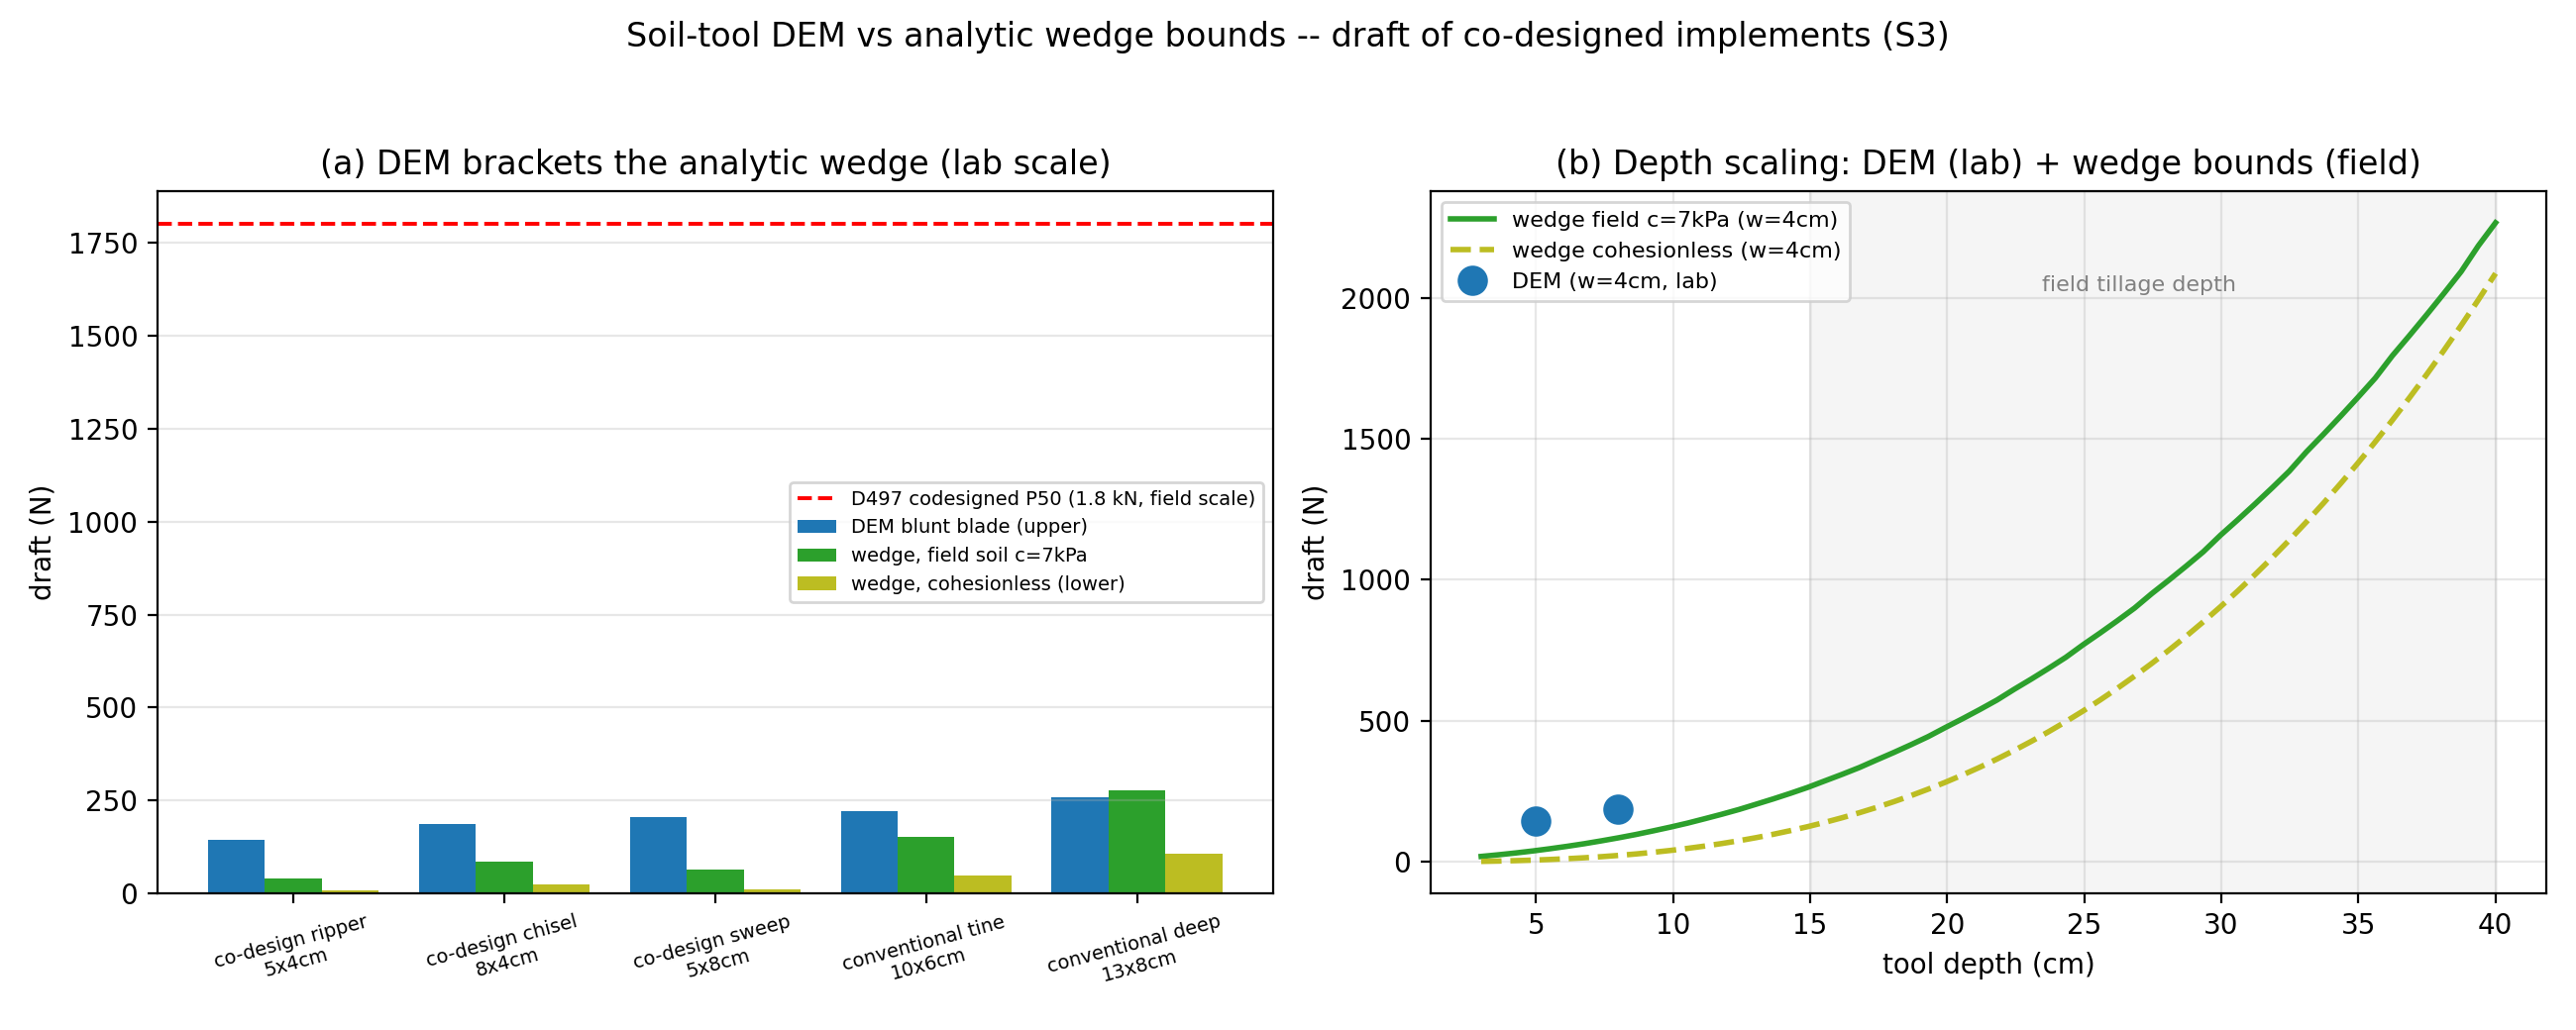
\includegraphics[width=0.95\linewidth]{F26_dem_draft}
\caption{Soil--tool DEM versus analytic wedge bounds (S3): (a) DEM draft brackets the slender-tine wedge (cohesionless lower bound and field-cohesion estimate) at lab scale; (b) depth scaling --- DEM lab points with the wedge bounds extrapolated to field depth, where the field-cohesion wedge meets the D497 codesigned reference.}
\label{fig:f26}
\end{figure}

\begin{figure}[H]
\centering
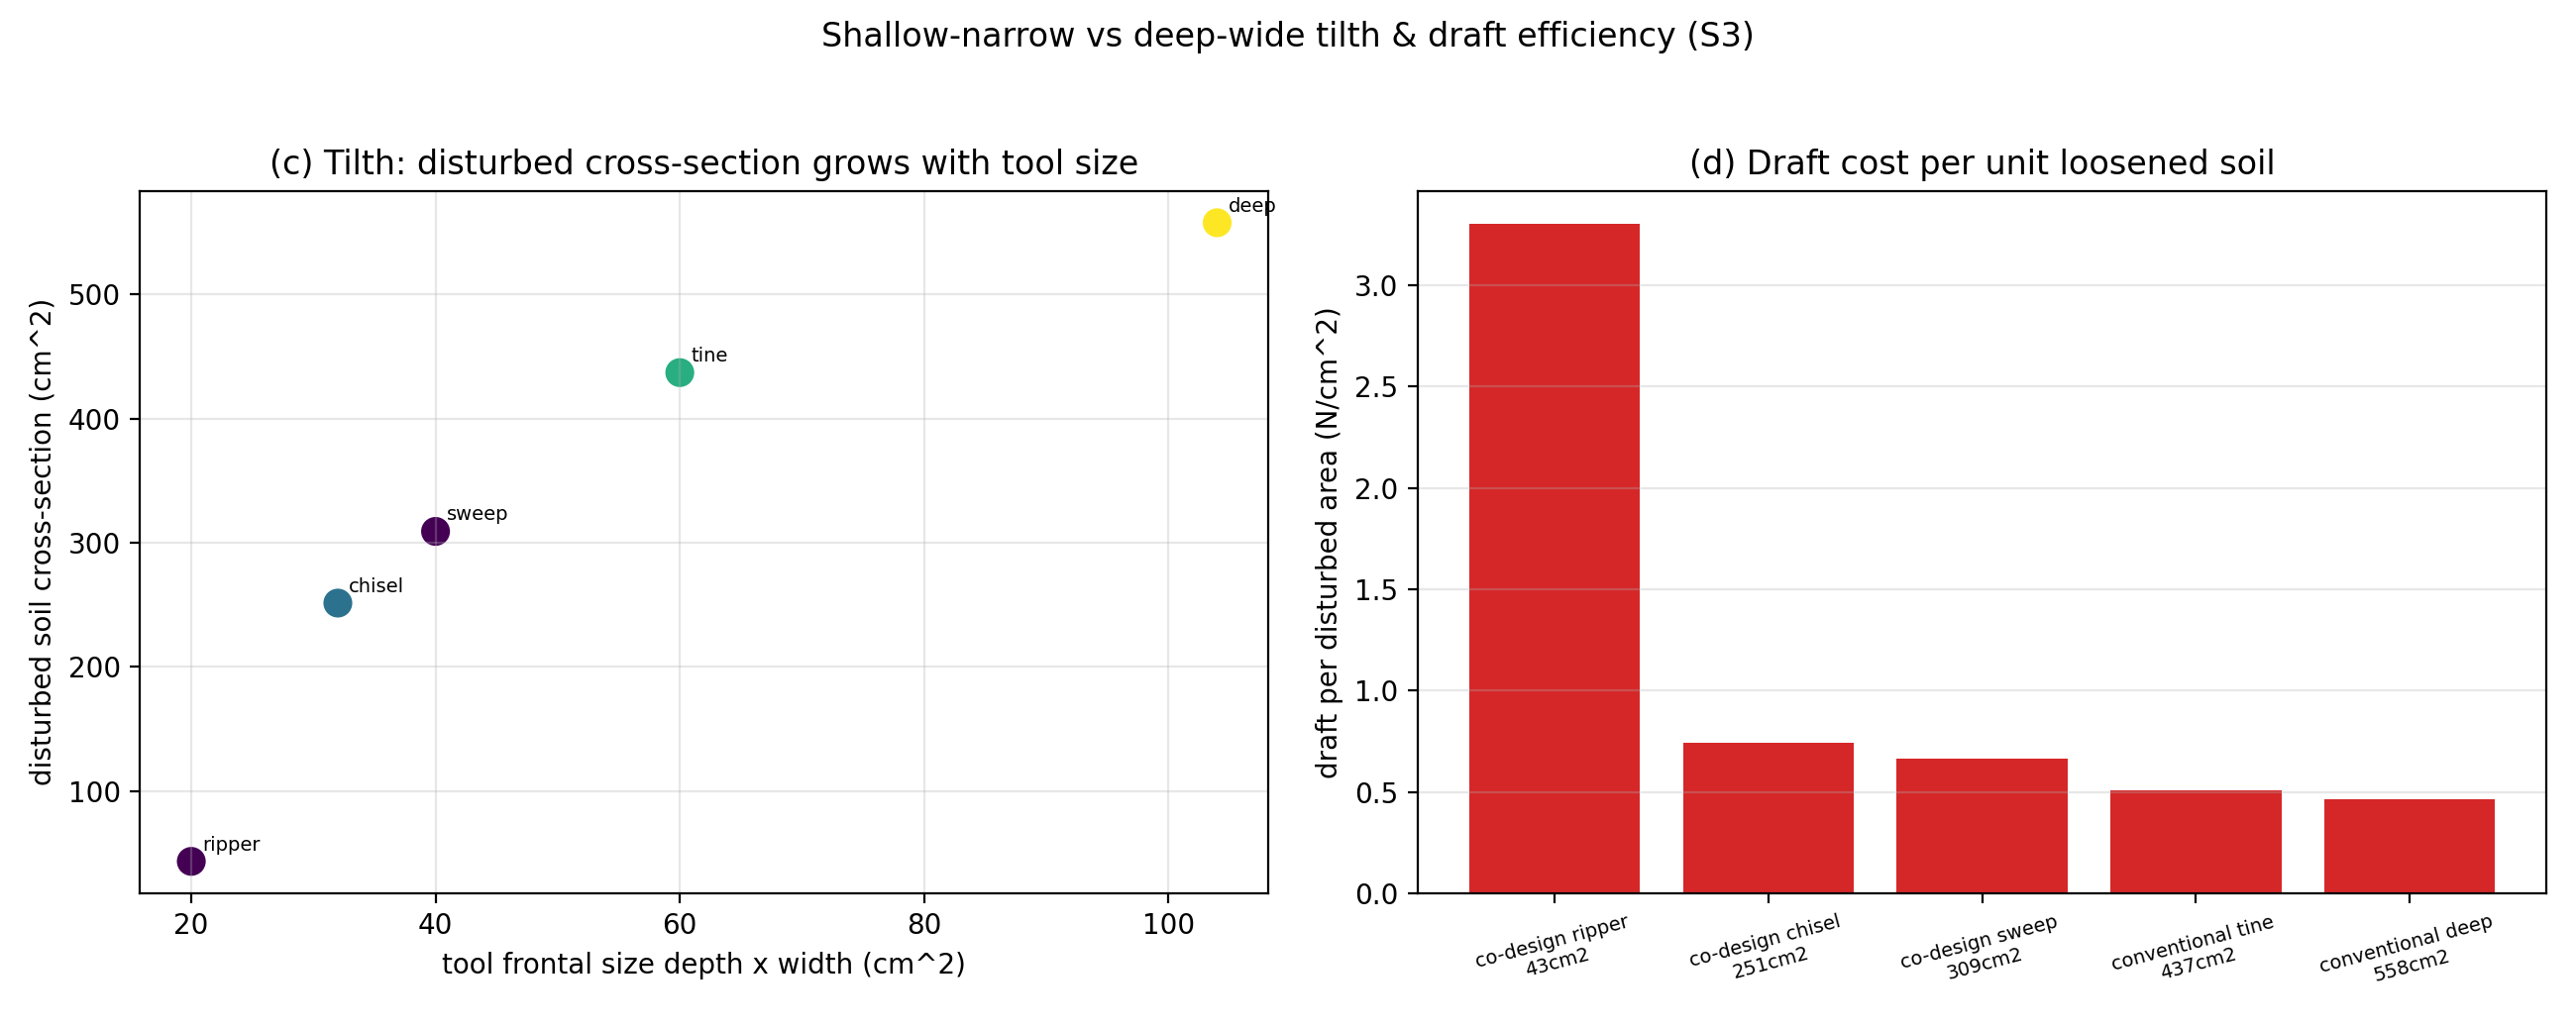
\includegraphics[width=0.95\linewidth]{F27_tilth_equivalence}
\caption{Shallow-narrow versus deep-wide tilth (S3): disturbed soil cross-section grows with tool size --- a shallow-narrow co-design pass disturbs ${\approx}10\times$ less soil than a deep-wide conventional one at ${\approx}0.65\times$ the draft --- and draft per unit disturbed area shows the narrow tool's higher cost per unit loosened soil.}
\label{fig:f27}
\end{figure}

\medskip
Taken together, these five studies tighten four of the open risks of \cref{sec:open-risks} (depth control, anchor capacity, cable safety, and co-design draft) and revise two artefacts of the screening analysis: the per-auger anchor nominal (\cref{sec:anchor}) and a previously missing cable-replacement cost line (\cref{sec:economics}). They do not close the risks --- a prototype season remains the arbiter --- but they replace ``not simulated'' with ``simulated at higher fidelity, with the following bounds.''

% ====================================================================
\section{Discussion}\label{sec:discussion}
% ====================================================================

\subsection{Where CableTract wins}\label{sec:wins}

The combined evidence of \cref{sec:r-c1,sec:r-c2,sec:r-c3,sec:r-c4,sec:r-envelope} points to a clear operating envelope:

\begin{itemize}[leftmargin=1.6em,itemsep=0.15em]
    \item \textbf{Operation type:} medium-load \emph{draft} operations --- light primary tillage (narrow ripper at ${\approx}\SI{3.0}{\kilo\newton}$ P50; chisel at \SI{4.2}{\kilo\newton} on medium-dense sites), all secondary tillage, seeding, and spraying (with a small carriage power pack, \cref{sec:carriage-power}). The rotary hoe and mower require powered-carriage variants and sit outside the headline envelope.
    \item \textbf{Farm size:} ${\gtrsim}\SI{40}{\hectare\per\year}$ annual operating area, where the replacement-frame \gls{npv} turns robustly positive (\cref{sec:npv-farmsize}); at \SI{100}{\hectare\per\year} the payback is \SI{2.5}{\year}. Below ${\approx}\SI{40}{\hectare\per\year}$ the machine is at best cost-neutral and the case must rest on compaction, autonomy, or decarbonisation value rather than cash flow.
    \item \textbf{Climate:} genuinely off-grid at high-irradiance sites (Konya class, ${\gtrsim}\SI{1650}{\kWh\per\meter\squared\per\year}$ at the reference hardware); near-off-grid with \SIrange{150}{282}{\hour\per\year} of backup, or off-grid with ${\approx}\SIrange{27}{30}{\meter\squared}$ of \gls{pv}, everywhere else we test (\cref{tab:site-summary}).
    \item \textbf{Field shape:} rectangular and L-shaped fields with $\geq\!\SI{1}{\hectare}$ individual size. Small fragmented fields hit the polygon shape efficiency wall (median $\eta \approx 0.68$ on the irregular-concave class), and headline numbers assume a span-commensurate rectangle (\cref{sec:layout-findings}).
\end{itemize}

\subsection{Where it doesn't (binding constraints)}\label{sec:loses}

Five constraints bind:

\begin{itemize}[leftmargin=1.6em,itemsep=0.15em]
    \item \textbf{Small annual areas.} Below ${\approx}\SI{40}{\hectare\per\year}$ the replacement-frame \gls{npv} is negative at all tested discount rates (\cref{tab:npv-farmsize}); the additive frame is negative everywhere within a single machine's capacity. This is the binding \emph{economic} constraint, and it was masked in an earlier revision by the uncosted carriage and an implement-blind capex parity.
    \item \textbf{Timeliness.} At \SI{12}{decares\per day}, one pass over \SI{25}{\hectare} takes ${\approx}21$ working days --- longer than typical seeding or spraying windows. A single unit therefore either serves a smaller in-window area (${\approx}\SIrange{10}{15}{\hectare}$ per 10--12-day window), shares window-critical operations with a contractor, or works in a multi-unit fleet; EP496-style timeliness penalties~\cite{asabe-ep496} for late seeding are of the same order as the entire annual cash saving and are not yet in the NPV chain (\cref{sec:analytical-limitations}).
    \item \textbf{Heavy codesigned primary tillage in loose-sand soils} sits outside the 9-screw free-head envelope (\cref{sec:anchor}): the narrow sweep (\SI{5.2}{\kilo\newton} P50), narrow chisel (\SI{4.2}{\kilo\newton}), narrow disk (\SI{3.2}{\kilo\newton}), and codesign drill (\SI{4.6}{\kilo\newton}) require 10--15 screws at the \SI{400}{\newton} bound (\cref{fig:f4}). With frame-coupled screws in medium-dense soil the same 9-screw Anchor carries the entire library with margin, so the binding case is loose-sand sites attempting heavy primary tillage with degraded head fixity.
    \item \textbf{Small fragmented fields} below ${\approx}\SI{1}{\hectare}$ individual size hit the polygon shape efficiency wall and lose ${\approx}\SI{30}{\percent}$ of nominal throughput (median irregular-concave $\eta \approx 0.68$). CableTract is not the right architecture for vegetable garden plots.
    \item \textbf{Operations needing power or precision at the tool.} Mowing (\SIrange{6}{7.5}{\kilo\watt} of cutting power, \cref{sec:carriage-power}) and cm-accurate row-following operations (\cref{sec:open-risks}, lateral guidance) are outside the present envelope pending a powered, guided carriage.
\end{itemize}

\subsection{Sensitivity to the central design choice}\label{sec:codesign-sensitivity}

The single most consequential choice in the paper is the \textbf{co-designed implement library}. Without the co-design framing --- that is, with conventional tractor implements substituted in place of the codesigned ones --- the analysis weakens in three concrete places:

\begin{enumerate}[leftmargin=1.6em,itemsep=0.1em]
    \item The \SI{2}{\kilo\watt} \gls{pmsm} is undersized (peak draft $\times$ tractor speed requires ${\approx}\SI{5}{\kilo\watt}$), and the inverter, gearbox, and cooling stack scale up with it.
    \item The energy-per-decare claim weakens substantially (S4: \SI{1227}{} $\to$ ${\approx}\SI{1721}{\Wh\per\decare}$ already at a $0.61\times$ achieved ratio), which directly weakens the off-grid PV+battery sizing.
    \item The 9-auger Anchor loses its worst-case-soil margin: a conventional chisel/sweep plow at \SIrange{14}{15}{\kilo\newton} P50 would need 41--45 augers on the worst-case Qureshi et al.\ (2024)~\cite{khand2024helical} loose-sand bound, although the same load fits in 9 augers on the Magnum (2024)~\cite{magnum2024fixed} medium-dense nominal.
\end{enumerate}

The first two items are the load-bearing ones --- they hold for \emph{any} soil regime. The replacement-frame \gls{npv} at a fixed \SI{25}{\hectare\per\year} workload is structurally draft-invariant in the off-grid frame (\cref{sec:v-s4}), but the off-grid story, the compaction story, and the motor sizing all weaken without co-design. The co-designed framing is therefore not a marketing convenience; it is the load-bearing assumption of the paper for energy and motor-cost reasons that are independent of soil conditions, with the worst-case-soil anchor envelope as a third leg. \Cref{sec:v-s4} quantifies the shortfall sensitivity through the full pipeline.

\subsection{What the paper does not claim}\label{sec:not-claim}

We do not claim:

\begin{itemize}[leftmargin=1.6em,itemsep=0.1em]
    \item That CableTract is a finished product or has been prototyped.
    \item That cable-driven agriculture is a new idea (steam cable ploughing predates it by 160 years~\cite{tyler1970steam}, and US 8,763,714 B2~\cite{orlando2014patent} predates this work).
    \item That the economics favour CableTract at small scale (they do not: the replacement-frame \gls{npv} is negative below ${\approx}\SI{40}{\hectare\per\year}$).
    \item That CableTract beats every competitor on every metric (the ecoRobotix class is more efficient per hectare on weeding-only; Na\"io is cheaper; \gls{ctf} captures much of the trafficked-area benefit with existing machinery).
    \item That off-grid operation is universal (it is climate-conditional; one bundled site achieves it at the reference hardware).
    \item That the $39\times$ field-integrated exposure reduction translates linearly into a yield increase (the soil-yield link depends on crop, climate, rotation, and irrigation).
\end{itemize}

We do claim, with every number reproducible from the open analytical pipeline:

\begin{itemize}[leftmargin=1.6em,itemsep=0.1em]
    \item Delivered electrical energy ${\approx}2.9\times$ below the diesel comparator's estimated drawbar work (${\sim}10\times$ on a primary-fuel basis, most of the extra factor being generic \gls{ice}-to-electric conversion efficiency), with the anchoring cycle charged.
    \item Roughly half the trafficked area at $4.6\times$ lower contact pressure --- a ${\approx}39\times$ field-integrated $p^2$-exposure reduction and a ${\approx}73\times$ per-running-gear index reduction.
    \item Off-grid operation at the highest-irradiance bundled site (\SI{58}{\hour\per\year} of grid support) and \SIrange{94}{98}{\percent} energy self-sufficiency at the other five, under a seasonal duty cycle, with \SI{15}{\meter\squared} \gls{pv} + \SI{9}{\kWh} battery.
    \item In the replacement frame, \gls{npv} negative below ${\approx}\SI{40}{\hectare\per\year}$, cost-neutral at \SI{25}{\hectare\per\year} (\SI{-1.7}{\kilo\EUR}), and positive above --- \SI{+9.1}{\kilo\EUR} with a \SI{2.5}{\year} payback at \SI{100}{\hectare\per\year} --- at 5/8/12\,\% discount rates.
    \item Lifecycle CO\textsubscript{2} $1.9\times$ lower than diesel, $1.6\times$ lower than a Monarch-class electric tractor.
    \item An operating envelope whose financial axis is a ${\approx}\SI{40}{\hectare\per\year}$ threshold (48\,\% of 3\,600 cells NPV-positive) and whose climate axis is the annual energy balance (${\approx}81\%$ of cells positive).
\end{itemize}

% ====================================================================
\section{Limitations}\label{sec:limitations}
% ====================================================================

This section separates two categories of limitation. \Cref{sec:analytical-limitations} lists the \emph{analytical} limitations of the present model --- what the framework does not include. \Cref{sec:open-risks} lists the \emph{engineering} risks that a prototype phase would have to resolve regardless of how comprehensive the analytical framework becomes; in the author's candid view these are the dominant near-term feasibility questions for the architecture and they are not closed by additional simulation.

\subsection{Analytical limitations of the present model}\label{sec:analytical-limitations}

\begin{enumerate}[leftmargin=1.8em,itemsep=0.2em]
    \item \textbf{No prototype.} The strongest objection. Every number in the paper is from first-principles calculation; none has been validated against a working machine. We have tried to mitigate this by using \gls{asabe} D497.7~\cite{asabe-d497} (an experimentally calibrated standard), the conservative end of the helical-anchor lateral capacity literature (Qureshi et al.\ 2024~\cite{khand2024helical} for loose-sand free-head bounds, Magnum Piering 2024~\cite{magnum2024fixed} design tables and the CHANCE Technical Design Manual~\cite{chance2024manual} for the medium-dense fixed-head reference), Keller and Lamand\'e (2010)~\cite{keller2010compaction} (experimentally measured tractor contact pressures), open published \gls{lca} inventories~\cite{hammond2019ice,emilsson2019battery,fraunhoferise2022pv,hawkins2013ev,defra2023factors,eea2023electricity}, and a Sobol global sensitivity analysis~\cite{sobol2001indices,saltelli2008primer,herman2017salib} to bound the uncertainty.
    \item \textbf{Reduced-order, not full multiphysics, control simulation.} \Cref{sec:v-s1} now adds a closed-loop depth-control co-simulation (a lumped-mass cable plus a unilateral gauge-wheel contact and a bandwidth-limited down-pressure actuator under PID and MPC), and \cref{sec:v-s7,sec:v-s2} add a nonlinear $p$--$y$ anchor model and a transient cable-recoil model. These are reduced-order, single-axis models validated against analytic limits, not a coupled full-multiphysics simulation of cable tension, three-dimensional anchor stability, and depth control together; that coupling, and its validation against hardware, remains for a prototype phase. \Cref{sec:open-risks} continues to treat the depth-control loop as the dominant unresolved risk, now bounded rather than unexamined.
    \item \textbf{Static contact-pressure compaction model.} No dynamic load transfer, no tyre deflection, no multi-pass cumulative deformation, no soil-yield link, and the carriage load excludes the vertical reaction of cable tension and tool downforce. The model is intentionally simple; a richer model would add compaction to the tractor side (multi-pass deformation) but also to the carriage side (repeated narrow-strip trafficking, added carriage downforce), so we do not assume it can only favour CableTract.
    \item \textbf{Polygon corpus is small and curated.} 50 fields, hand-tuned, biased toward small awkward shapes. A real deployment would need a corpus pulled from EuroCrops or \gls{usda} at scale.
    \item \textbf{PV harvest model in the operating-envelope sweep is a one-parameter linear fit.} The full hourly TMY pipeline lives in \cref{sec:energy} and was used for \cref{fig:f6,fig:f7,fig:f8}, but the (annual \gls{ghi} $\times$ farm size) sweep in \cref{fig:f21} uses a calibrated linear approximation for tractability. The $\alpha = 0.169$ value was fitted as the median across the 6 bundled sites.
    \item \textbf{The codesigned implement library is a paper exercise.} The 10 implements are sized using the \gls{asabe} D497.7 equation but have not been physically built. The draft reductions are predictions, not measurements.
    \item \textbf{The competitor comparison uses public-domain manufacturer claims.} Some of these may not reproduce in the field. The source of every number is flagged in the bundled competitor table.
    \item \textbf{Timeliness, labour, and residual values are outside the cash-flow chain.} EP496-style timeliness penalties~\cite{asabe-ep496} for window-critical operations, operator labour (a cost for the tractor, a supervision requirement of unresolved legal scope for CableTract), and year-15 residual values are all excluded; the first two are individually of the same order as the reference-point annual saving and are discussed qualitatively in \cref{sec:loses,sec:tornado}.
    \item \textbf{The anchoring model is geotechnically narrow.} The $p$--$y$ study covers dry sand only (no cohesive or saturated profiles, though spring tillage happens in wet soil), uses static rather than cyclic resistance factors, applies ad hoc safety factors (1.15 envelope / 1.5 nominal) rather than a standards-grade limit-state framework~\cite{ac358,perko2009helical}, and omits the sheave-height overturning couple's axial push--pull on the screw group. A per-placement torque-verification protocol (each screw drive is a torque-instrumented installer) plus a brief cable proof-tension before each strip would convert spatial soil variability into an acceptance test, and is recommended for the prototype.
\end{enumerate}

\subsection{Open mechanical risks}\label{sec:open-risks}

The seven items above are the analytical limitations of the present model: they describe what the framework does not include. This subsection separates out a different category --- \textbf{the engineering risks that a prototype phase would actually have to resolve}, regardless of how comprehensive the analytical framework becomes. We list them explicitly so a follow-on team can attack them in priority order rather than re-deriving the list from the manuscript.

\paragraph{Closed-loop tilling depth control.} Tilling depth at the carriage is governed by the geometric coupling between cable sag, cable elastic stretch, carriage horizontal position, implement reaction torque, and the time-varying soil contact force. None of these are independent variables, and none were simulated under closed-loop control in the original screening model. \Cref{sec:catenary,sec:tension-balance} bound the static sag-vs-tension trade-off under nominal loads, but do not address the dynamic response to a transient draft spike --- a buried stone, a hardpan layer, a moisture gradient. Unlike a tractor with a 3-point hitch and several tonnes of vehicle inertia to absorb the spike, the cable carriage has neither inertia nor a stiff mechanical reference frame; the response is mediated entirely by cable elasticity and the winch motor's torque-control bandwidth. Whether the resulting tilling quality meets agronomic acceptance criteria is, in the author's view, the single largest unresolved technical risk in the architecture. It is also one of the cheapest to test: a quarter-scale bench rig on a \SI{5}{\meter} span in a soil bin is sufficient to bound it before any full-scale prototype is built. The closed-loop co-simulation added in \cref{sec:v-s1} now bounds this risk analytically: it confirms the cable is far too soft to set depth (so a gauge wheel must), shows that a tuned controller holds the \(\pm\SI{2}{\centi\meter}\) tolerance through stone, hardpan, and moisture disturbances, and isolates the residual failure mode --- transient gauge-wheel lift-off during a sharp draft spike --- which is removed by carrying a steady down-pressure reserve of ${\approx}\SI{1.75}{\kilo\newton}$ at a ${\geq}\SI{5}{\hertz}$ actuator bandwidth. The bench rig remains the right validation step; what changes is that it now has a quantitative target to confirm rather than an open question to explore.

\paragraph{Per-strip setup time as a design target rather than a measurement.} The model uses $t_{\text{setup}} = \SI{60}{\second}$ as the per-round overhead (\cref{tab:codesigned-params}). This is a \emph{design target}, not a field measurement, and the architecture in \cref{sec:two-module} relies on the only configuration that makes it plausible: nine \emph{parallel} screw drives on the Anchor (one \gls{bldc} per screw, all nine cycling concurrently) and four parallel drives on the Main Unit. With parallel driving, the per-round cycle decomposes into ${\sim}\SI{20}{\second}$ insert $+$ ${\sim}\SI{10}{\second}$ retract for the screw cycle (\cref{sec:anchoring-energy}), ${\sim}\SI{5}{\second}$ for the lateral step, ${\sim}\SI{5}{\second}$ for cable slack take-up, ${\sim}\SI{5}{\second}$ for \gls{gnss} re-survey, and ${\sim}\SI{5}{\second}$ for re-tensioning --- about \SI{50}{\second} of nominal work inside the \SI{60}{\second} budget. Even at the target, setup is a first-order share of both the time budget (${\approx}\SIrange{27}{43}{\percent}$, \cref{sec:layout-findings}) and the energy budget (27\,\%, \cref{sec:anchoring-energy}); if field measurements come in slower, both degrade proportionally. Three residual concerns survive and should be measured by a prototype campaign before this number is treated as solved. (i) The single-auger insert/retract time at this duty cycle is unmeasured in the public literature; if it turns out to be significantly longer than \SI{30}{\second} on representative soils, the entire 60 s budget shifts. (ii) The margin inside the budget is small enough that any non-augering surprise --- a tangled cable, a carriage hookup failure, a stale \gls{gnss} fix --- consumes the slack on the round it occurs. (iii) Auger insertion time on hard-pan or stony soils is non-linear in cone index in ways the present model does not capture. The Sobol sweep (\cref{sec:sobol}) brackets setup time over \SIrange{30}{180}{\second}, which covers the realistic uncertainty around the parallel-drive nominal but does not extend to the failure mode where parallel augering itself is slower than assumed. The CableTract+ variant in \cref{sec:variants-named} eliminates the per-strip Anchor reset entirely and is, in part, a structural insurance policy against this concern rather than an independent throughput play.

\paragraph{Lateral guidance and row registration.} The cable's transverse point stiffness at midspan is the same ${\approx}4T/L \approx \SI{144}{\newton\per\meter}$ the depth-control study derives for the vertical axis, so an asymmetric soil reaction of only ${\sim}\SI{100}{\newton}$ --- routine for tillage tools in heterogeneous soil --- can displace the pull point laterally by the better part of a metre. Nothing in the present design steers the carriage: \gls{gnss} sits on the modules, not the carriage, and no coulter, furrow-follower, or row-perception element is specified. Draft-dominated broadacre operations tolerate decimetre-level wander, but seeding-then-hoeing on the same rows requires centimetre-level pass-to-pass registration, and any guidance solution (steerable coulters, carriage \gls{gnss}, row cameras) adds ground-engaging elements, mass, and cost. We rank this risk alongside depth control --- it is the second axis of the same problem --- and it must be part of the same soil-bin campaign.

\paragraph{Anchor self-fatigue of its own anchoring soil.} The Anchor's lateral capacity envelope (\cref{sec:anchor}) treats per-auger lateral capacity as a property of soil texture and density alone. In normal operation, however, each Anchor station drives and retracts nine augers tens to hundreds of times across a cropping season as the Anchor walks the headland. The cumulative effect is that the soil under each station is progressively loosened by the system's own operation: a soil that began as medium-dense (and therefore sat comfortably inside the Magnum 2024~\cite{magnum2024fixed} envelope at $5$--$10\times$ margin) drifts toward the loose-sand regime (Qureshi 2024~\cite{khand2024helical} envelope at ${\sim}\,1\times$ margin) as the season progresses. The 9-auger design margin erodes \emph{from inside}, not from changes in field conditions. Quantifying the rate at which this happens requires either an empirical campaign on a fixed Anchor station or a finite-element model of repeated helical pile insertion and withdrawal; neither is in the present paper, and the architecture's worst-case soil envelope should be read with this caveat in mind.

\paragraph{Helical pile retraction wear.} Helical screw piles in the construction industry are designed and qualified for one-shot installation with permanent service. CableTract drives and retracts each auger many cycles per day, which is a regime for which no fatigue, helix wear, shaft buckling, or soil-disturbance data exists in the public literature the author could find. The first-order risks are blunting of the helix leading edge (which would slow each subsequent insertion and increase the auger drive's torque demand), shaft fatigue at the drive coupling, and progressive misalignment of the helix from the shaft axis. The framing is that this is an unmeasured failure mode rather than necessarily a small one --- there is no published basis to estimate the mean time between auger replacements, and the bill of materials in \cref{sec:economics} does not include an auger replacement schedule. A first prototype campaign should treat auger wear as a primary measurement endpoint alongside throughput and energy.

\paragraph{Historical cable ploughing as an unaddressed precedent.} The architecture has a precedent the present paper has not yet fully engaged with. Steam-driven cable ploughing was a real and widely deployed technology in the second half of the 19th century, particularly on heavy clay soils in the United Kingdom and parts of continental Europe where horse teams bogged. Two stationary steam engines at opposite headlands pulled a two-bottom plough back and forth on a steel cable (the Fowler and Howard cable-ploughing systems). The system coexisted with horse and traction-engine ploughing for several decades and then disappeared, comprehensively, by the early 20th century. The reasons usually given for its decline --- which we cite here from secondary recollection rather than a primary historical source we have verified, and flag as such --- are per-station crew overhead, the time cost of repositioning the engines after each strip, the management burden of the cable itself, and the inability to turn at the headland and resume continuously. The present manuscript automates the per-station crew problem (the Main Unit and Anchor are autonomous) but does not yet solve the repositioning, cable-management, or continuous-headland-turn problems that killed the steam-era version. A serious treatment of this lineage --- what cable ploughing did, why it failed, what is mechanically and operationally different now --- belongs in any prototype-stage publication. We flag its absence here as a deliberate scope decision and a known weakness.

\paragraph{Cable safety surface.} A \SI{50}{\meter} Dyneema cable at \SIrange{1.5}{4}{\kilo\newton} working tension running across an open field at ${\approx}\SI{0.8}{\meter}$ above the ground is a safety surface the original screening model did not address. Snap-back energy from a cable failure is non-trivial at these tensions, and a deployed system would need cable-condition monitoring, runaway-detection logic, exclusion zones, and certification under the relevant agricultural-machinery regulatory framework. None of this is in scope here, but it would be a precondition for any field deployment and would add both \gls{bom} cost and certification process cost. \Cref{sec:v-s2} now quantifies the dominant terms: snap-back recoil velocities (counter-intuitively higher for the lighter synthetic rope) set the required full-span exclusion zone; the bending-fatigue life is shown to be UV/abrasion-limited at ${\approx}\SI{8}{\year}$ rather than fatigue-limited, which supplies the previously-missing cable-replacement cost and life-cycle line (\cref{sec:economics}); and an aeroelastic check flags vortex-induced vibration (requiring dampers) and an iced-galloping constraint (de-tension in icing). These bound the safety surface analytically but do not substitute for the monitoring, certification, and field validation a deployment still requires.

\medskip
The unifying observation is that the strongest near-term feasibility questions for CableTract are \textbf{mechanical and operational}, not financial or environmental. The paper's NPV, life-cycle CO\textsubscript{2}, and energy-per-hectare numbers are robust within their stated framework; the open question is whether the framework's mechanical assumptions survive contact with a real prototype season. We make this distinction explicit so a reviewer can evaluate the analytical contribution on its own merits while understanding which questions a prototype-stage follow-up would actually need to answer.

% ====================================================================
\section{Conclusion}\label{sec:conclusion}
% ====================================================================

This paper presents a prototype-free, fully reproducible feasibility envelope for \textbf{CableTract}, a co-designed cable-driven field robot consisting of a stationary \gls{mu}, a lighter Anchor held by retractable ground screws, and a soil-supported implement carriage towed along a tensioned cable loop between them. The central design lever is the \textbf{co-designed implement library} --- 10 implements sized for the cable architecture rather than borrowed from conventional tractor inventories --- which reduces median per-pass draft by ${\approx}\,63\%$ (the tension-budget lever that makes the cable, motor, and anchor feasible) and brings the entire library inside the 9-screw Anchor envelope on the frame-coupled medium-dense reference, with the lighter half also fitting the worst-case loose-sand envelope.

The codesigned reference achieves:

\begin{itemize}[leftmargin=1.6em,itemsep=0.15em]
    \item \textbf{\SI{1227}{\Wh\per\decare}} delivered electrical energy with the anchoring cycle charged (${\approx}2.9\times$ below the diesel comparator's estimated drawbar work, ${\sim}10\times$ below its primary fuel energy; \SI{1259}{\Wh\per\decare} without regen).
    \item \textbf{Roughly half the trafficked area at $4.6\times$ lower contact pressure} --- a \textbf{${\approx}\,39\times$ field-integrated reduction in $p^2$-weighted soil-stress exposure} --- uniformly across field classes, positioning the architecture as an extreme, low-pressure form of controlled traffic.
    \item \textbf{Off-grid operation at the sunniest bundled site (\SI{58}{\hour\per\year} of grid support) and \SIrange{94}{98}{\percent} energy self-sufficiency at the other five}, under a seasonal duty cycle with \SI{15}{\meter\squared} \gls{pv} and \SI{9}{\kWh} of battery.
    \item \textbf{Scale-conditional replacement economics}: cost-neutral at \SI{25}{\hectare\per\year} (NPV \SI{-1.7}{\kilo\EUR}), break-even near \SI{40}{\hectare\per\year}, \SI{+9.1}{\kilo\EUR} at \SI{100}{\hectare\per\year}; an additive buyer cannot amortise a single machine within its own capacity.
    \item \textbf{Lifecycle CO\textsubscript{2} of \SI{17.0}{\kilogram\per\hectare\per\year}} versus 32.5 for diesel --- a $1.9\times$ improvement that does not depend on grid decarbonisation.
\end{itemize}

The operating envelope of \cref{fig:f21} integrates these into the paper's central result: a \emph{farm-size} threshold near \SI{40}{\hectare\per\year} on the financial axis (48\,\% of the 3\,600 swept cells NPV-positive; ${\approx}12\%$ under the additive frame) and an annual energy balance on the climate axis (${\approx}81\%$ of cells positive). The corrected accounting of this revision --- anchoring energy, per-swath trafficking, the costed carriage, frame-consistent purchase scenarios, and a seasonal duty cycle --- moves every headline toward more modest, more defensible values, and in doing so exposes the architecture's real design lever: the per-round anchoring cycle, which consumes 27\,\% of the energy and roughly a third of the time budget. The multi-strip beam variant that amortises it (\cref{sec:variant-beam}) recovers most of the loss --- \SI{974}{\Wh\per\decare} and $1.21\times$ throughput for a \SI{1.5}{\kilo\EUR} increment --- and is gated only on verifying the beam's yaw-moment load path, which the prototype campaign below can test with the same instrumented screws.

The right next step is \textbf{a Main Unit prototype} with a \SI{2}{\kilo\watt} \gls{pmsm}, a \SI{9}{\kWh} pack, a 9-screw Anchor, and the codesigned narrow ripper as the first implement, deployed on a ${\gtrsim}\SI{40}{\hectare}$ rectangular block at a high-irradiance site (Konya class) for one full cropping season --- instrumented for the four measurements this paper cannot make: draft under load at cable speeds, closed-loop depth \emph{and lateral} behaviour of the carriage, screw insert/retract time--torque--wear statistics, and realised energy harvest. Until then, the analytical envelope above is the best defensible feasibility case for the architecture.

% ====================================================================
\appendix
% ====================================================================
\section{Architectural variants considered}\label{sec:variants-named}
% ====================================================================

The architectural family has several siblings worth naming. Regenerative braking on the return leg is part of the default baseline (\cref{sec:drivetrain}). Three configurations are quantitatively compared against that baseline in \cref{sec:ml,fig:f20} --- multi-strip anchoring (beam + travelling sheave, \cref{sec:variant-beam}), CableTract+, and the unidirectional (no-regen) drivetrain. A naive swivelling-sheave realisation of multi-strip anchoring (pivot on a point-anchored module) is retained in \texttt{cabletract/variants.py} for completeness but is geometrically unsound as a coverage mechanism (\cref{sec:variants-intro}); a drone-assisted inter-field alignment variant is deferred to future work, together with two further concepts.

\begin{table}[H]
\centering\small
\caption{Architectural variants and their modelling status. ``Compared'' means the variant is implemented as a parameter transformation on the codesigned reference, evaluated in \cref{sec:ml}, and shown alongside the baseline in \cref{fig:f20}.}\label{tab:variants}
\begin{tabularx}{\textwidth}{lXl}
\toprule
Variant & Description & Status \\
\midrule
\textbf{Regenerative return leg} & Four-quadrant motor operation recovering energy on the unloaded carriage return / downhill slope. & \textbf{Default (baseline)} \\
\textbf{Multi-strip anchoring (beam)} & Both modules anchor once per $k$-strip block; a sheave trolley on a rigid transverse beam indexes the take-off point between strips (\cref{sec:variant-beam}). & Compared ($k=4$) \\
\textbf{CableTract+} & Four corner Main Units pulling the carriage with two simultaneously-active cables --- eliminates the Anchor and the per-strip anchoring cycle. & Compared \\
\textbf{Unidirectional (no regen)} & The baseline with the regen drive removed; one-way drivetrain, \SI{300}{\EUR} cheaper, ${\approx}2.6\%$ higher (slope-averaged) energy. & Compared \\
Swivelling pulley (naive) & Sheave pivots on a point-anchored module so the cable fans to successive strip lines; geometrically unsound for coverage (passes overlap near the pivot, \cref{sec:variants-intro}) --- superseded by the beam variant. & Excluded \\
Drone-assisted alignment & A small quadcopter drops \gls{gps} markers between fields so re-alignment takes seconds. & Deferred (setup-side) \\
Liquid-hose extension & The cable doubles as a liquid feed for spraying or fertigation. & Deferred \\
In-place rotary mode & The carriage spins around the \gls{mu} on a single tether for circular operations such as orchard mowing. & Deferred \\
\bottomrule
\end{tabularx}
\end{table}

% ====================================================================
\section{List of acronyms}\label{sec:acronyms}
% ====================================================================
\printglossary[type=\acronymtype,title={},toctitle={List of acronyms}]

% ====================================================================
\section*{CRediT authorship contribution statement}
% ====================================================================
\textbf{Özgür Yılmaz:} Conceptualization, Methodology, Software, Formal analysis, Investigation, Validation, Visualization, Writing --- original draft, Writing --- review \& editing.

% ====================================================================
\section*{Declaration of competing interest}
% ====================================================================
The author declares that he has no known competing financial interests or personal relationships that could have appeared to influence the work reported in this paper.

% ====================================================================
\section*{Funding}
% ====================================================================
This research did not receive any specific grant from funding agencies in the public, commercial, or not-for-profit sectors.

% ====================================================================
\section*{Data and code availability}
% ====================================================================
The complete analytical code, all bundled input data (\gls{tmy} summaries, \gls{asabe} D497 coefficients, ground-screw capacities, cable mechanical properties, \gls{bom} CO\textsubscript{2} intensities, and the field-polygon corpus), and every figure and result table in this manuscript can be regenerated from a clean checkout by running the phase scripts (\texttt{run\_phase1}--\texttt{run\_phase12}); per-figure CSV companions are written to \texttt{tables/}. The repository is openly available at \cabletractrepo and is archived at Zenodo (DOI to be assigned on acceptance).

% ====================================================================
\section*{Declaration of generative AI and AI-assisted technologies in the manuscript preparation process}
% ====================================================================
During the preparation of this work the author used a large language model (Anthropic Claude) to assist with implementing and structuring the analytical code, drafting and editing prose, and organising the presentation of results. After using this tool, the author reviewed and verified all output against the executed code, edited it as needed, and takes full responsibility for the content of the published article.

% ====================================================================
% References — heading is provided by \begin{thebibliography}
% ====================================================================

\begin{thebibliography}{99}\setlength{\itemsep}{0.18em}

% --- Patents and standards ---
\bibitem{orlando2014patent}
R.~Orlando and A.~Zoffoli,
\emph{Agricultural traction system with cable and hoists},
U.S. Patent 8\,763\,714 B2, July 2014.

\bibitem{asabe-d497}
American Society of Agricultural and Biological Engineers,
\emph{ASABE Standard D497.7: Agricultural Machinery Management Data},
ASABE, St.\ Joseph, MI, March 2011 (R2015).

\bibitem{asabe-ep496}
American Society of Agricultural and Biological Engineers,
\emph{ASABE Engineering Practice EP496.3: Agricultural Machinery Management},
ASABE, St.\ Joseph, MI, 2006 (R2020).

% --- Helical pile lateral capacity ---
\bibitem{khand2024helical}
H.\,A. Qureshi, M. Safdar, M. Haseeb, M.\,T. Bashir, M.\,A. Khan, Z. Khatak, H. Bilal, M. Alam, and M.\,M.\,H. Khan,
``Lateral capacity of group helical piles in sand: an experimental and numerical study for sustainable infrastructures,''
\emph{International Journal of Geotechnical Engineering}, vol.~18, nos.~7--10, pp.~728--742, 2024.
\href{https://doi.org/10.1080/19386362.2024.2406372}{doi:10.1080/19386362.2024.2406372}.

\bibitem{magnum2024fixed}
Magnum Piering, Inc.,
\emph{Magnum Helical Pile Allowable Lateral Shaft Capacity (lbs) --- Fixed-Head Condition},
product datasheet, October 2024 revision (manufacturer document; not peer-reviewed). Accessed June 2026.
\href{https://magnumpiering.com/wp-content/uploads/2024/10/Lateral\%20Shaft\%20Capacity\%20Fixed.pdf}{magnumpiering.com}.

\bibitem{chance2024manual}
Hubbell Power Systems / CHANCE Foundation Solutions,
\emph{CHANCE Technical Design Manual}, 5th ed.,
Hubbell Power Systems, Centralia, MO, 2024, 337\,pp. (industry design manual; not peer-reviewed).

% --- Cable mechanics and rope hardware ---
\bibitem{irvine1981cables}
H.\,M. Irvine,
\emph{Cable Structures},
MIT Press, Cambridge, MA, 1981.

\bibitem{feyrer2015wireropes}
K. Feyrer,
\emph{Wire Ropes: Tension, Endurance, Reliability}, 2nd ed.,
Springer, Berlin Heidelberg, 2015.
\href{https://doi.org/10.1007/978-3-642-54996-0}{doi:10.1007/978-3-642-54996-0}.

% --- Implement draft and machinery management ---
\bibitem{kheiralla2004tillage}
A.\,F. Kheiralla, A. Yahya, M. Zohadie, and W. Ishak,
``Modelling of power and energy requirements for tillage implements operating in Serdang sandy clay loam, Malaysia,''
\emph{Soil and Tillage Research}, vol.~78, no.~1, pp.~21--34, 2004.

\bibitem{siemens1999machinery}
J.\,C. Siemens and W. Bowers,
\emph{Machinery Management: How to Select Machinery to Fit the Real Needs of Farm Managers},
Farm Business Management series, Deere \& Company, Moline, IL, 1999.

% --- Solar geometry, clear sky and wind ---
\bibitem{cooper1969absorption}
P.\,I. Cooper,
``The absorption of solar radiation in solar stills,''
\emph{Solar Energy}, vol.~12, no.~3, pp.~333--346, 1969.

\bibitem{haurwitz1945insolation}
B. Haurwitz,
``Insolation in relation to cloudiness and cloud density,''
\emph{Journal of Meteorology}, vol.~2, no.~3, pp.~154--166, 1945.

\bibitem{justus1978winds}
C.\,G. Justus,
\emph{Winds and Wind System Performance},
Franklin Institute Press, Philadelphia, PA, 1978.

% --- Soil compaction ---
\bibitem{sohne1953druck}
W. S\"ohne,
``Druckverteilung im Boden und Bodenverformung unter Schlepperreifen,''
\emph{Grundlagen der Landtechnik}, no.~5, pp.~49--63, 1953.

\bibitem{keller2010compaction}
T. Keller and M. Lamand\'e,
``Challenges in the development of analytical soil compaction models,''
\emph{Soil and Tillage Research}, vol.~111, no.~1, pp.~54--64, 2010.

% --- Life-cycle inventories and energy economics ---
\bibitem{hammond2019ice}
G.\,P. Hammond and C.\,I. Jones,
\emph{Inventory of Carbon and Energy (ICE)}, version~3.0,
University of Bath / Circular Ecology, Bath, UK, 2019.

\bibitem{emilsson2019battery}
E. Emilsson and L. Dahll\"of,
\emph{Lithium-Ion Vehicle Battery Production: Status 2019 on Energy Use, CO\textsubscript{2} Emissions, Use of Metals, Products' Environmental Footprint, and Recycling},
IVL Swedish Environmental Research Institute, Report C\,444, Stockholm, 2019.

\bibitem{fraunhoferise2022pv}
Fraunhofer Institute for Solar Energy Systems ISE,
\emph{Photovoltaics Report},
Freiburg, Germany, updated February 2022.

\bibitem{hawkins2013ev}
T.\,R. Hawkins, B. Singh, G. Majeau-Bettez, and A.\,H. Str{\o}mman,
``Comparative environmental life cycle assessment of conventional and electric vehicles,''
\emph{Journal of Industrial Ecology}, vol.~17, no.~1, pp.~53--64, 2013.

\bibitem{defra2023factors}
UK Department for Environment, Food \& Rural Affairs,
\emph{UK Government GHG Conversion Factors for Company Reporting --- 2023},
DEFRA, London, 2023.

\bibitem{eea2023electricity}
European Environment Agency,
\emph{Greenhouse Gas Emission Intensity of Electricity Generation in Europe},
EEA, Copenhagen, 2023.

\bibitem{bnef2024battery}
BloombergNEF,
\emph{Lithium-ion Battery Price Survey 2024},
Bloomberg New Energy Finance, December 2024.

% --- Sensitivity analysis ---
\bibitem{sobol2001indices}
I.\,M. Sobol',
``Global sensitivity indices for nonlinear mathematical models and their Monte Carlo estimates,''
\emph{Mathematics and Computers in Simulation}, vol.~55, nos.~1--3, pp.~271--280, 2001.
\href{https://doi.org/10.1016/S0378-4754(00)00270-6}{doi:10.1016/S0378-4754(00)00270-6}.

\bibitem{saltelli2008primer}
A. Saltelli, M. Ratto, T. Andres, F. Campolongo, J. Cariboni, D. Gatelli, M. Saisana, and S. Tarantola,
\emph{Global Sensitivity Analysis: The Primer},
John Wiley \& Sons, Chichester, UK, 2008.

\bibitem{herman2017salib}
J. Herman and W. Usher,
``SALib: an open-source Python library for sensitivity analysis,''
\emph{Journal of Open Source Software}, vol.~2, no.~9, p.~97, 2017.
\href{https://doi.org/10.21105/joss.00097}{doi:10.21105/joss.00097}.

\bibitem{iwanaga2022salib}
T. Iwanaga, W. Usher, and J. Herman,
``Toward SALib 2.0: advancing the accessibility and interpretability of global sensitivity analyses,''
\emph{Socio-Environmental Systems Modelling}, vol.~4, p.~18155, 2022.
\href{https://doi.org/10.18174/sesmo.18155}{doi:10.18174/sesmo.18155}.

% --- Higher-fidelity verification studies (Sec. 8) ---
\bibitem{murchison1984evaluation}
J.\,M. Murchison and M.\,W. O'Neill,
``Evaluation of p--y relationships in cohesionless soils,''
in \emph{Analysis and Design of Pile Foundations} (J.\,R. Meyer, ed.),
ASCE, New York, 1984, pp.~174--191.

\bibitem{api2014rp2a}
American Petroleum Institute,
\emph{Recommended Practice for Planning, Designing and Constructing Fixed Offshore Platforms --- Working Stress Design}, API RP 2A-WSD, 22nd ed.,
API, Washington, DC, 2014.

\bibitem{reese1974analysis}
L.\,C. Reese, W.\,R. Cox, and F.\,D. Koop,
``Analysis of laterally loaded piles in sand,''
in \emph{Proc.\ 6th Offshore Technology Conference}, Houston, TX, 1974, paper OTC~2080, pp.~473--483.
\href{https://doi.org/10.4043/2080-MS}{doi:10.4043/2080-MS}.

\bibitem{reese2011single}
L.\,C. Reese and W.\,F. Van Impe,
\emph{Single Piles and Pile Groups Under Lateral Loading}, 2nd ed.,
CRC Press / Taylor \& Francis, London, 2011.

\bibitem{mokwa1999resistance}
R.\,L. Mokwa,
\emph{Investigation of the Resistance of Pile Caps to Lateral Loading},
Ph.D.\ dissertation, Virginia Polytechnic Institute and State University, Blacksburg, VA, 1999.

\bibitem{hetenyi1946beams}
M. Het\'enyi,
\emph{Beams on Elastic Foundation},
University of Michigan Press, Ann Arbor, MI, 1946.

\bibitem{denhartog1956mechanical}
J.\,P. Den Hartog,
\emph{Mechanical Vibrations}, 4th ed.,
McGraw-Hill, New York, 1956 (reprinted Dover, 1985).

\bibitem{blevins1990flow}
R.\,D. Blevins,
\emph{Flow-Induced Vibration}, 2nd ed.,
Van Nostrand Reinhold, New York, 1990.

\bibitem{reece1965fundamental}
A.\,R. Reece,
``The fundamental equation of earth-moving mechanics,''
\emph{Proc.\ Institution of Mechanical Engineers}, vol.~179, part~3F, pp.~16--22, 1965.

\bibitem{godwin1977soil}
R.\,J. Godwin and G. Spoor,
``Soil failure with narrow tines,''
\emph{Journal of Agricultural Engineering Research}, vol.~22, no.~3, pp.~213--228, 1977.
\href{https://doi.org/10.1016/0021-8634(77)90044-0}{doi:10.1016/0021-8634(77)90044-0}.

\bibitem{mckyes1985soil}
E. McKyes,
\emph{Soil Cutting and Tillage}, Developments in Agricultural Engineering~7,
Elsevier, Amsterdam, 1985.


\bibitem{schjonning2012rules}
P. Schj\o nning, M. Lamand\'e, T. Keller, J. Pedersen, and M. Stettler,
``Rules of thumb for minimizing subsoil compaction,''
\emph{Soil Use and Management}, vol.~28, no.~3, pp.~378--393, 2012.
\href{https://doi.org/10.1111/j.1475-2743.2012.00411.x}{doi:10.1111/j.1475-2743.2012.00411.x}.

\bibitem{tullberg2007ctf}
J.\,N. Tullberg, D.\,F. Yule, and D. McGarry,
``Controlled traffic farming --- From research to adoption in Australia,''
\emph{Soil and Tillage Research}, vol.~97, no.~2, pp.~272--281, 2007.
\href{https://doi.org/10.1016/j.still.2007.09.007}{doi:10.1016/j.still.2007.09.007}.

\bibitem{chamen2015mitigating}
W.\,C.\,T. Chamen, A.\,P. Moxey, W. Towers, B. Balana, and P.\,D. Hallett,
``Mitigating arable soil compaction: A review and analysis of available cost and benefit data,''
\emph{Soil and Tillage Research}, vol.~146, pp.~10--25, 2015.
\href{https://doi.org/10.1016/j.still.2014.09.011}{doi:10.1016/j.still.2014.09.011}.

\bibitem{mcphee2020lowmass}
J.\,E. McPhee, D.\,L. Antille, J.\,N. Tullberg, R.\,B. Doyle, and M. Boersma,
``Managing soil compaction --- A choice of low-mass autonomous vehicles or controlled traffic?,''
\emph{Biosystems Engineering}, vol.~195, pp.~227--241, 2020.
\href{https://doi.org/10.1016/j.biosystemseng.2020.05.006}{doi:10.1016/j.biosystemseng.2020.05.006}.

\bibitem{pott2018cdpr}
A. Pott,
\emph{Cable-Driven Parallel Robots: Theory and Application},
Springer Tracts in Advanced Robotics, vol.~120. Cham: Springer, 2018.
\href{https://doi.org/10.1007/978-3-319-76138-1}{doi:10.1007/978-3-319-76138-1}.

\bibitem{albus1993robocrane}
J. Albus, R. Bostelman, and N. Dagalakis,
``The NIST RoboCrane,''
\emph{Journal of Robotic Systems}, vol.~10, no.~5, pp.~709--724, 1993.
\href{https://doi.org/10.1002/rob.4620100509}{doi:10.1002/rob.4620100509}.

\bibitem{kirchgessner2017fip}
N. Kirchgessner, F. Liebisch, K. Yu, J. Pfeifer, M. Friedli, A. Hund, and A. Walter,
``The ETH field phenotyping platform FIP: a cable-suspended multi-sensor system,''
\emph{Functional Plant Biology}, vol.~44, no.~1, pp.~154--168, 2017.
\href{https://doi.org/10.1071/FP16165}{doi:10.1071/FP16165}.

\bibitem{tyler1970steam}
C. Tyler and J. Haining,
\emph{Ploughing by Steam: A History of Steam Cultivation Over the Years}.
Hemel Hempstead: Model \& Allied Publications, 1970.

\bibitem{lane1980fowler}
M.\,R. Lane,
\emph{The Story of the Steam Plough Works: Fowlers of Leeds}.
London: Northgate Publishing, 1980.

\bibitem{lagnelov2021cost}
O. Lagnel\"ov, G. Larsson, D. Nilsson, A. Larsolle, and P.-A. Hansson,
``Cost analysis of autonomous battery electric field tractors in agriculture,''
\emph{Biosystems Engineering}, vol.~204, pp.~358--376, 2021.
\href{https://doi.org/10.1016/j.biosystemseng.2021.02.005}{doi:10.1016/j.biosystemseng.2021.02.005}.

\bibitem{lowenberg2020economics}
J. Lowenberg-DeBoer, I.\,Y. Huang, V. Grigoriadis, and S. Blackmore,
``Economics of robots and automation in field crop production,''
\emph{Precision Agriculture}, vol.~21, pp.~278--299, 2020.
\href{https://doi.org/10.1007/s11119-019-09667-5}{doi:10.1007/s11119-019-09667-5}.

\bibitem{perko2009helical}
H.\,A. Perko,
\emph{Helical Piles: A Practical Guide to Design and Installation}.
Hoboken, NJ: John Wiley \& Sons, 2009.

\bibitem{ac358}
ICC Evaluation Service,
\emph{AC358: Acceptance Criteria for Helical Pile Systems and Devices}.
Brea, CA: ICC-ES, 2017.

\bibitem{aguiar1988markov}
R.\,J. Aguiar, M. Collares-Pereira, and J.\,P. Conde,
``Simple procedure for generating sequences of daily radiation values using a library of Markov transition matrices,''
\emph{Solar Energy}, vol.~40, no.~3, pp.~269--279, 1988.
\href{https://doi.org/10.1016/0038-092X(88)90049-7}{doi:10.1016/0038-092X(88)90049-7}.

\end{thebibliography}

\end{document}
